\documentclass{beamer}

\usepackage{amsmath}
\usepackage{amssymb}
\usepackage{graphicx}
\usepackage{subcaption}
\usepackage{float}
\usepackage{multirow}
\usepackage{alphalph}
\usepackage{listings}

\usepackage{appendixnumberbeamer}


\usepackage{xcolor}


\usetheme{Frankfurt}
%\xdefinecolor{maroon}{cmyk}{0.15,1.00,0.39,0.69}
%\xdefinecolor{maroon}{cmyk}{0.27,0.86,0.60,0.30}
%\xdefinecolor{maroon}{cmyk}{0.000,1.00,1.00,0.498}
\usecolortheme[RGB={80,0,0}]{structure}

\newcommand{\highlight}[1]{%
  \colorbox{red!50}{$\displaystyle#1$}}


% Shortcut commands
% My Shortcut Commands
\newcommand{\fig}[1]{Fig.~\ref{#1}}                      % figure
\newcommand{\tbl}[1]{Table~\ref{#1}}                     % table

\newcommand{\be}{\begin{equation*}}   % numbered equation
\newcommand{\ee}{\end{equation*}}

\newcommand{\benum}{\begin{equation}}   % numbered equation
\newcommand{\eenum}{\end{equation}}

\newcommand{\bea}{\begin{eqnarray*}}  % numbered equation array
\newcommand{\eea}{\end{eqnarray*}}

\newcommand{\beanum}{\begin{eqnarray}}  % numbered equation array
\newcommand{\eeanum}{\end{eqnarray}}

\newcommand{\eqt}[1]{Eq. (\ref{#1})}  % Reference to one equation
\newcommand{\eqts}[1]{Eqs. (\ref{#1})}  % Reference to multiple equations 

\newcommand{\B}[1]{\ensuremath{b_{#1} }}			% B with a sub scripted argument

\newcommand{\R}[1]{\ensuremath{\mathbf{R}_{#1}}}
\newcommand{\D}{\ensuremath{ \mathbf{D}_* }}
\newcommand{\I}{\ensuremath{ \mathbf{I} }}
\newcommand{\M}{\ensuremath{ \mathbf M}}

\newcommand{\p}{\ensuremath{ \partial}}			% shortcut partial derivative symbol

\newcommand{\abs}[1]{\ensuremath{\left\lvert #1 \right\rvert}}  % absolute value of argument (variable bar size)
\newcommand{\norm}[1]{\ensuremath{\left\lVert #1 \right\rVert}}  % norm of argument, varaible size


% Equation Punctuation
\newcommand{\pec}{\, ,}
\newcommand{\pep}{\, .}
\setbeamertemplate{footline}{
\leavevmode%
\hbox{\hspace*{-0.06cm}
\begin{beamercolorbox}[wd=.45\paperwidth,ht=2.25ex,dp=1ex,center]{author in head/foot}%
	\usebeamerfont{author in head/foot}Maginot%~~(\insertshortinstitute)
\end{beamercolorbox}%
\begin{beamercolorbox}[wd=.3\paperwidth,ht=2.25ex,dp=1ex,center]{section in head/foot}%
PhD Defense %\usebeamerfont{section in head/foot}\insertshorttitle
\end{beamercolorbox}%
\begin{beamercolorbox}[wd=.25\paperwidth,ht=2.25ex,dp=1ex,right]{section in head/foot}%
	\usebeamerfont{section in head/foot}April 2015\hspace*{2em}
	\insertframenumber{} / \inserttotalframenumber\hspace*{2ex}
\end{beamercolorbox}}%
\vskip0pt%
}
\beamertemplatenavigationsymbolsempty
\beamertemplatetransparentcovered

\setbeamertemplate{bibliography item}[text]

\title{Higher Order Grey Thermal Radiative Transfer}
\author{Peter Maginot}\institute{Texas A\&M University- Department of Nuclear Engineering}
\date{April 2015}


\newif\ifplacelogo % create a new conditional
\placelogotrue % set it to true
\logo{\ifplacelogo
\includegraphics[height=1cm]{CSGF_vert.pdf} \hspace{3.5in} 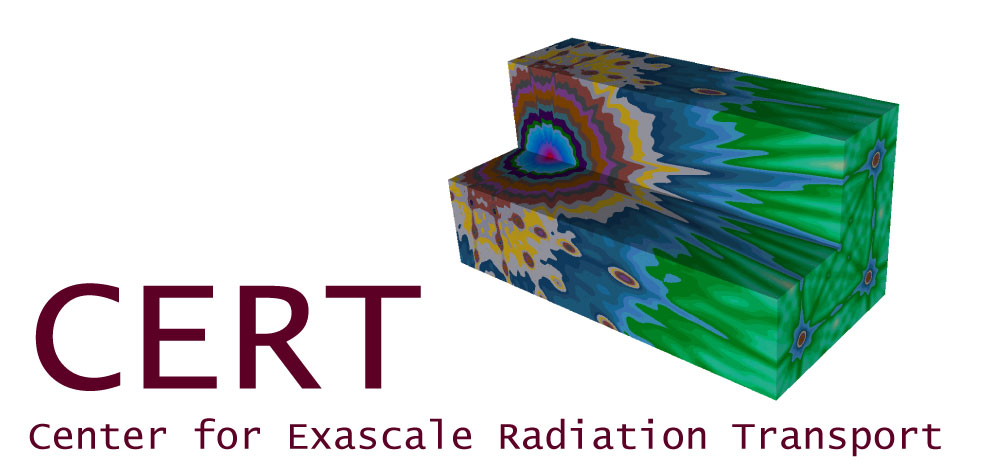
\includegraphics[height=1cm]{cert-logo}\fi}

\begin{document}
%---------------------------------------------------------------------------------------------
\placelogotrue
\begin{frame}
\titlepage


\end{frame}

%---------------------------------------------------------------------------------------------

\placelogofalse
%---------------------------------------------------------------------------------------------
\begin{frame}
\frametitle{Outline}
\tableofcontents[hideallsubsections]
%\begin{enumerate}
%\item Spatially Varying Cross Section Problems
%\item Low Order DSA for High Order DFEM Transport
%\item Strictly Non-Negative Bilinear Scheme for Unstrutured Quads
%\end{enumerate}
\end{frame}

\section{Theory}

\subsection{Goal}

\begin{frame}
\begin{block}{Dissertation Goal}
\begin{center}
High-fidelity methods for discrete ordinates ($S_N$) radiative transfer
\end{center}
\end{block}
\begin{center}
\begin{Large}
\bf
Requirements to Achieve Goal
\end{Large}
\end{center}
\begin{enumerate}
\item Accurate Spatial Discretization
\begin{itemize}
\item Higher degree trial space discontinuous finite element method (DFEM) trial spaces
\item Must address robustness
\end{itemize}
\item Accurate Spatial Treatment of Opacities
\begin{itemize}
\item Cell-wise constant is a poor approximation for problems of interest
\end{itemize}
\item Efficient / Effective Acceleration
\begin{itemize}
\item Computationally efficient
\item Compatible with spatial discretization
\end{itemize}
\end{enumerate}

\end{frame}

\subsection{Matrix Lumping}
\begin{frame}
\frametitle{Matrix Lumping}

\begin{enumerate}
\item One of three methods to improve the DFEM ``robustness'' 
\begin{itemize}
\item Other methods: ad-hoc fix-ups, strictly non-negative solution representations
\item Robustness (for $S_N$): solution positivity and resistance to oscillations
\end{itemize}
\item Lumping- makes diagonal mass matrices, does not guarantee increase in robustness
\item Two ways to lump mass matrices
\begin{itemize}
\item Traditional lumping (TL): Collapse an exactly integrated mass matrix's entries to the main diagonal
\item Self-lumping (SL): Use quadrature restricted to the DFEM interpolation points
\end{itemize} 
\item Both methods are equivalent for linear DFEM
\end{enumerate}
\end{frame}

\begin{frame}
\frametitle{Self-Lumping Concept}
With interpolatory basis functions, restricting quadrature to the DFEM interpolation points ($s_j$) creates a diagonal mass matrix ($\mathbf{M}$) {\em automatically}
\begin{block}{Self-lumping (SL) $\mathbf{M}$}
\be
\mathbf{M}_{ij} = \left \{ \begin{array}{ll}  \frac{\Delta x }{2} w_i  & i=j \\ 0 & \text{otherwise} \end{array} \right.
\ee
\end{block}
\begin{itemize}
\item Typically, $s_j$ are chosen as equally-spaced points, and $\mathbf{M}$ is integrated analytically
\item No requirement that $s_j$ be equally-spaced, could use more accurate quadrature as the interpolation points
\begin{itemize}
\item E.g. Gauss-Legendre (Gauss) or Lobatto-Gauss-Legendre (Lobatto)
\end{itemize}
\end{itemize}
\end{frame}

\subsection{Robustness}
\begin{frame}
\frametitle{Numerical Schemes}
\begin{block}{New to Dissertation}
\begin{small}
\begin{itemize} 
\item Self-lumping with higher degree trial spaces
\item Non equally-spaced interpolation points
\end{itemize}
\end{small}
\end{block}
\begin{itemize}
\item {\bf SL Gauss}: Gauss quadrature as interpolation points, quadrature restricted to interpolation points
\item {\bf SL Lobatto}: Lobatto quadrature as interpolation points, quadrature restricted to interpolation points
\item {\bf SL Newton-Cotes}: Equally-spaced points, quadrature (closed Newton-Cotes) restricted to interpolation points
\item {\bf TL} (Traditional Lumping): Equally-spaced points, analytic integration, then collapse to main diagonal
\item {\bf Exact DFEM}: Equally-spaced points, analytic integration
\end{itemize}
\end{frame}


\begin{frame}
\frametitle{Outflow Robustness}
\begin{columns}[c]
\column{0.5\textwidth}
\begin{figure}
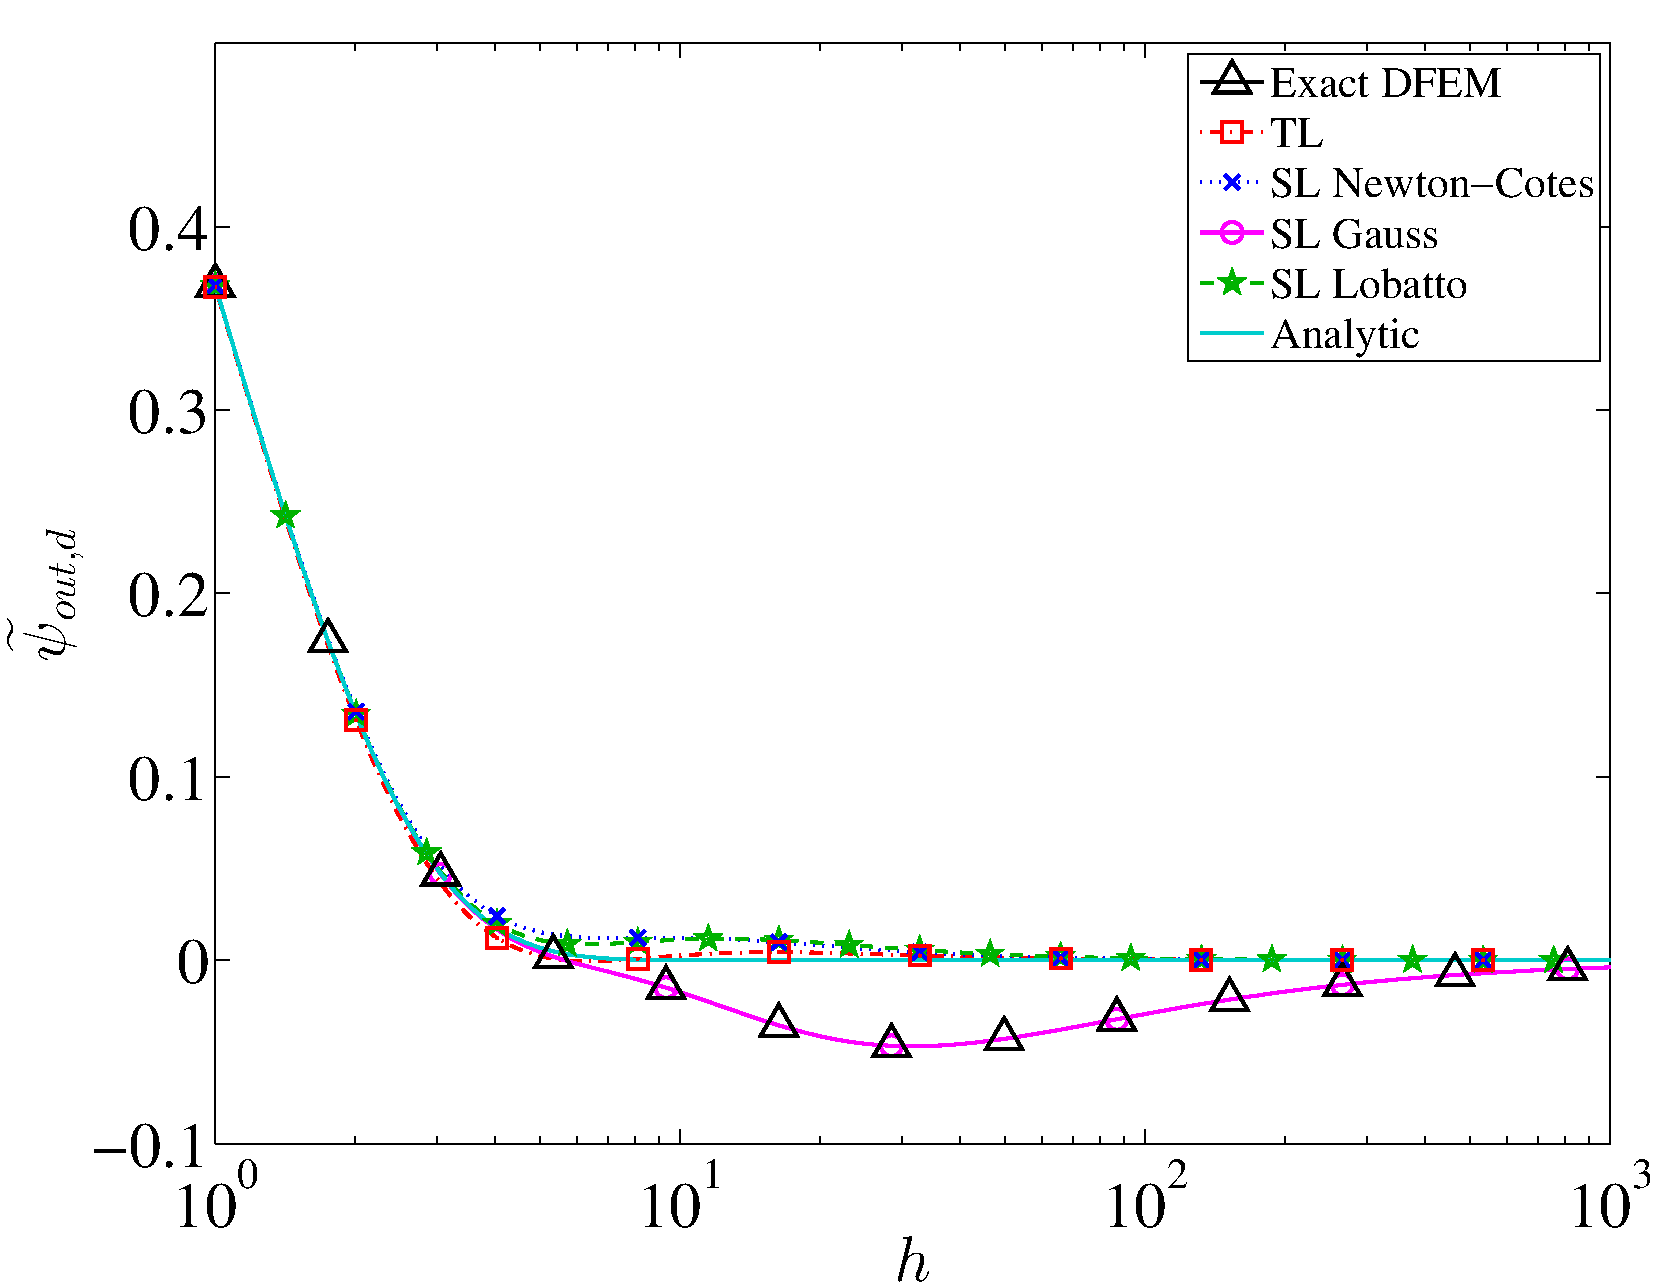
\includegraphics[width=5.5cm]{../chapter2_constant_xs/P3_Outflow_AllMeth-eps-converted-to.pdf}
\caption{$P=3$ Outflow as a function of $h$.}
\end{figure}
\column{0.5\textwidth}
\begin{figure}
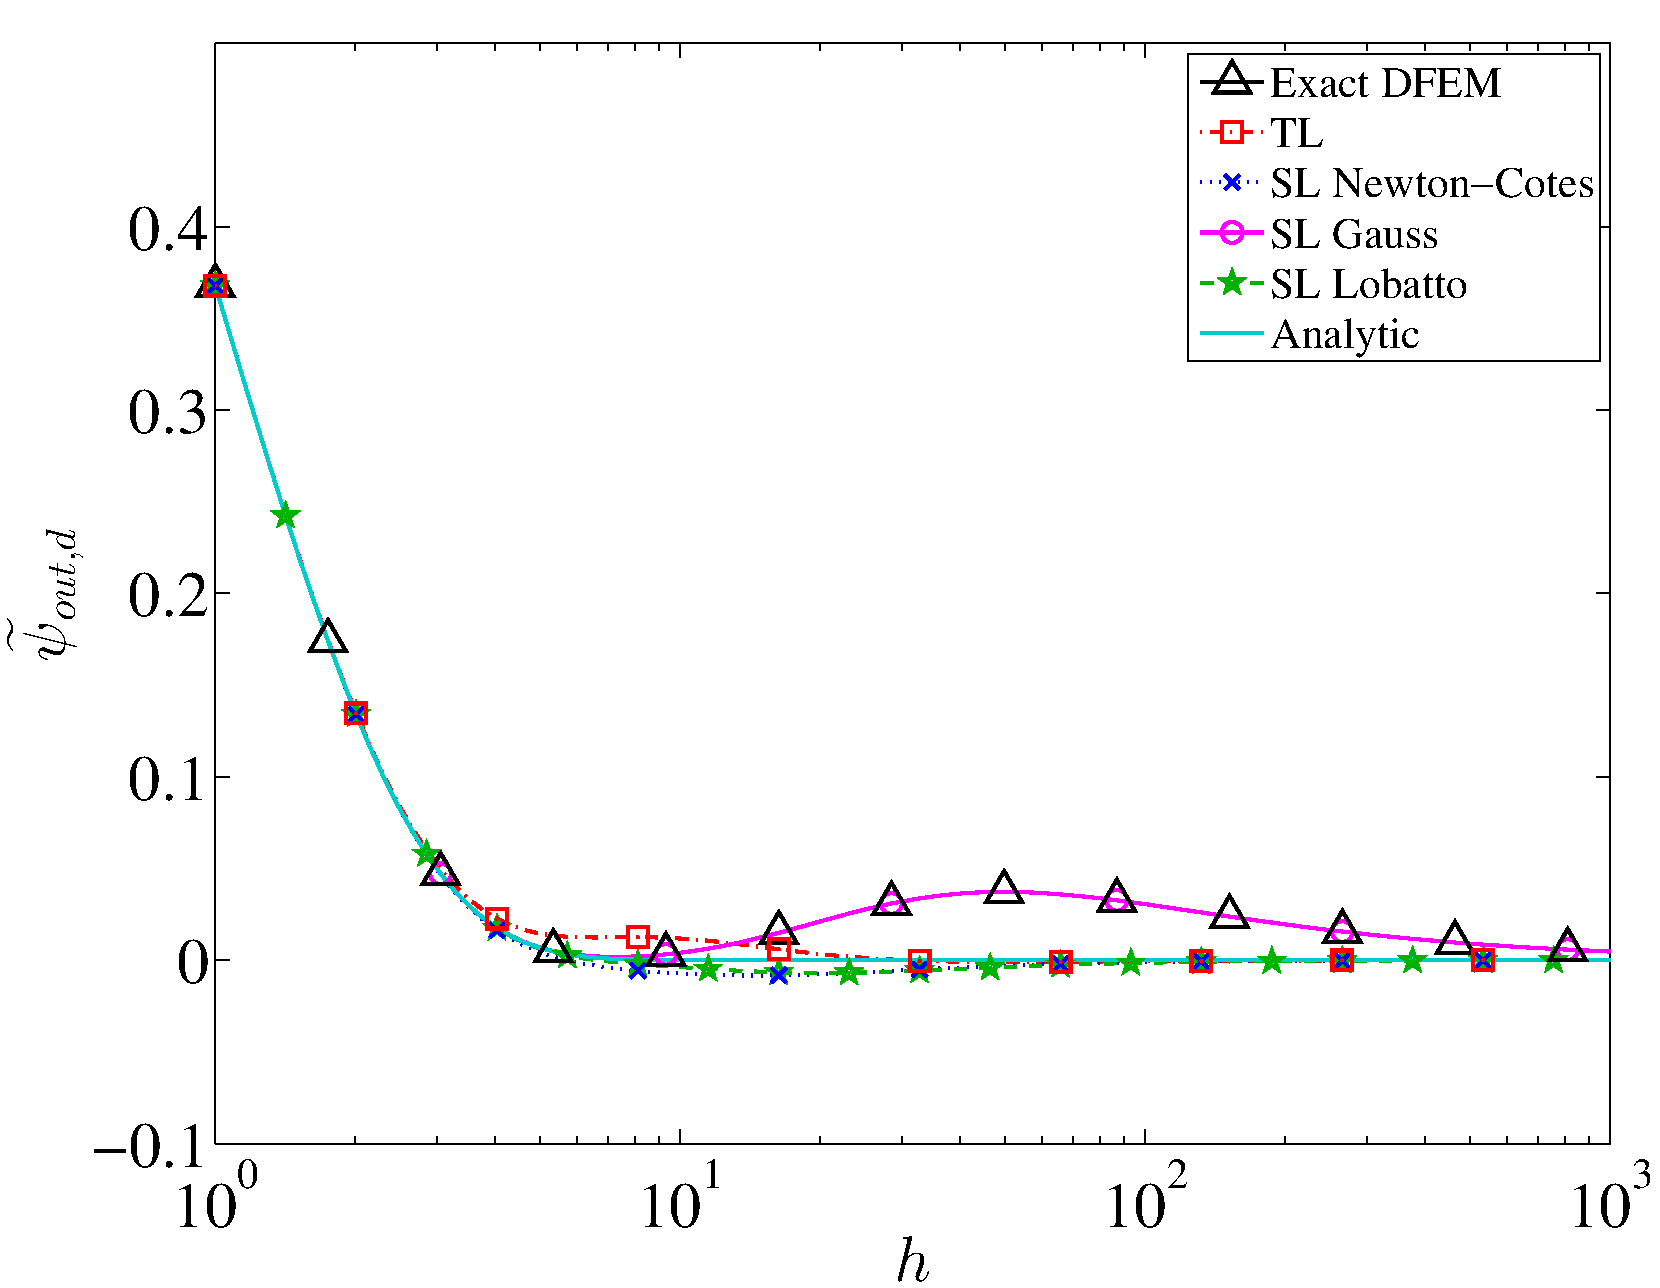
\includegraphics[width=5.5cm]{../chapter2_constant_xs/P4_Outflow_AllMeth-eps-converted-to.pdf}
\caption{$P=4$ Outflow as a function of $h$.}
\end{figure}
\end{columns}
\end{frame}


\subsection{Spatially Varying Cross Section}

\begin{frame}
\frametitle{Motivation to Account for Cross Section Spatial Variation}
\begin{itemize}
\item Many problems of interest to the NE community have within cell spatially varying cross section/opacity
\begin{itemize}
\item Cross sections are functions of temperature, density, fuel burn-up, etc.
\item High fidelity simulations do not assume cell-wise constant values for these variables
\end{itemize}
\item Neutronics examples: fuel depletion problems, coupled reactor physics...
\item Radiative transfer: $\sigma = T^{-3}$
\end{itemize}
\end{frame}

\begin{frame}
\frametitle{$S_N$ Reaction Term}
In DFEM spatial discretization of $S_N$ transport and thermal radiative transfer equations, we have interactions terms like:
\benum
\frac{\Delta x}{2} \int_{-1}^{1}{\sigma(s) \B{i}(s) \widetilde{\psi}(s)~ds} 
\label{eq:exact_r}
\eenum
Historically, for a $P$ degree polynomial trial space representation with $N_P = P+1$ degrees of freedom, this is approximated as
\benum
\bar{\sigma} \mathbf{M} \vec{\psi}
\label{eq:old_r}
\eenum
where 
\be
\vec{\psi} = \left[ \psi_1 \dots \psi_{N_P+1} \right]^T,~~\widetilde{\psi}(s) = \sum_{j=1}^{N_P}{\B{j}(s) \psi_j}
\ee
\eqt{eq:old_r} exact iff $\sigma(s) = \bar{\sigma}$. 
\end{frame}

\begin{frame}
\frametitle{History}
In neutronics:
\begin{itemize}
\item Some work has focused on assuming cross section is a linear function within cells
\item Focus of this historical work has been on reproducing fine mesh results with coarser zoning
\end{itemize}
Radiative transfer/radiative diffusion calculations (sometimes) account for within cell variation by using vertex based quadrature integration
\begin{itemize}
\item Idea introduced by Adams and Nowak circa 1997
\item Used by some (ex. Ober and Shadid ~2004)
\item Not by everyone
\end{itemize}
\end{frame}

\subsection{Extending Self-Lumping Framework}

\begin{frame}
\frametitle{SL Schemes for Spatially Varying Cross Section Problems}
\vspace{-0.1in}
\eqt{eq:exact_r} correctly represented as:
\vspace{-0.1in}
\be
\mathbf{R}_{\sigma}\vec{\psi}
\ee 
with
\vspace{-0.1in}
\be
\mathbf{R}_{ij} = \frac{\Delta x}{2}\int_{-1}^1{ \sigma(s) \B{i}(s) \B{j}(s)~ds}
\ee
\vspace{-0.1in}
%
\begin{block}{Self-Lumping Cross Section (SLXS) Schemes}
Extension of self-lumping schemes to account for spatial variation of opacity/cross section
\be
\mathbf{R}_{\sigma,ij}= \left \{ \begin{array}{ll}  \frac{\Delta x }{2}\sigma(s_i) w_i  & i=j \\ 0 & \text{otherwise} \end{array} \right.
\ee
\end{block}
\begin{itemize}
\item {\bf SLXS Lobatto}- self-lumping incorporating spatial variation of material properties, Lobatto DFEM interpolation points 
\item {\bf SLXS Gauss}- self-lumping incorporating spatial variation of material properties, Gauss DFEM interpolation points
\end{itemize}
%
\end{frame}

\section{TRT Equations}

\subsection{Analytic TRT}
\begin{frame}
\frametitle{Grey Thermal Radiative Transfer Equations}
Grey (frequency integrated) thermal radiative transfer (TRT) equations:
\bea
\frac{1}{c} \frac{\partial I}{\p t} + \mu_d \frac{\p I}{\p x}  + \sigma_t I &=&  2\pi \int_{-1}^{1}{ \sigma_s(\mu'\to\mu_d) I  d\mu }+ \sigma_a B + S_I\\
C_v \frac{\p T}{\p t} &=&   \sigma_a \left( \phi- 4\pi B   \right) + S_T
\eea
\begin{columns}[t]
\column{0.6\textwidth}
\footnotesize
$I(x,\mu_d,t)$- intensity $\left[ \frac{energy}{area-time-ster} \right]$ \\
$\phi(x,t)$- angle integrated intensity $\left[ \frac{energy}{area-time} \right]$ \\
$B(T) = \frac{acT^4}{4\pi}$- Planck function $\left[ \frac{energy}{area-time-ster} \right]$ \\
$C_v(x,T)$- heat capacity $\left[ \frac{energy}{volume-temperature} \right] $
\column{0.5\textwidth}
\footnotesize
$T(x,t)$- temperature \\
$\sigma_{a}(x,T)$- absorption opacity  $\left[ {length}^{-1} \right]$ \\
$\sigma_{s}(x,T)$- scattering opacity  $\left[ {length}^{-1} \right]$ 
\end{columns}
\end{frame}


\begin{frame}
\frametitle{Solution Methodology}
\begin{enumerate}
\item Linearize Planckian in temperature
\small
\bea
B(T) &\approx& B(T_*) + \frac{d B}{d T} \bigg \lvert_{T=T_*} (T - T_*)\\
B_*& =& B(T_*),~D_* = \frac{d B}{d T} \bigg \lvert_{T=T_*} \\
B &\approx& B_* + D_*(T-T_*)
\eea
\normalsize
\item Expand Planckian in $P$ degree trial space
\small
\be
B(\widetilde{T}) \approx \sum_{j=1}^{N_P}{ B(T_j) \B{j}(s) }
\ee
\normalsize
\item Linearize (for given temperature iterate) radiation equation using temperature equation 
\item Ignore material properties contributions to Jacobian
\item Assume SDIRK time integration
\item Newton-Picard iteration for temperature
\end{enumerate}
\end{frame}

\subsection{SDIRK}
\begin{frame}
\frametitle{SDIRK- S-stable Diagonally Implicit Runge-Kutta}
\small
Solves problems of the form:
\bea
g(t=0) &=& g_0 \\
g'(t) &=& f(t,g)
\eea
With the following relations
\benum
g_{n+1} = g_n + \Delta t \sum_{i=1}^{N_{stage}}{b_i k_i} 
\label{eq:sdirk_middle}
\eenum
\be
k_i = f\left( t_n + c_i \Delta t ~,~g_{n} + \Delta t \sum_{j=1}^i{a_{ij} k_j }\right) 
\ee
\eqt{eq:sdirk_middle} can also be interpreted as:
\be
g_i = g_{n} + \Delta t \sum_{j=1}^i{a_{ij} f\left(t_n + \Delta t c_j , g_j\right)} \pec
\ee
$a_{ij}$,~$b_i$,~$c_{i}$ are all constants inherent to a given scheme
\end{frame}

\subsection{Spatially Analytic Linearization}
\begin{frame}
\frametitle{TRT Time Discretization}
Manipulating analytic equations, $k$ of stage $s$ are:
\bea
k_{I,s} &=& c\left[ \frac{1}{4\pi}\sigma_{s}(T_s) \phi_s + \sigma_a(T_s) B(T_s) + S_I(t_s) - \mu_d \frac{\partial I_s}{\partial x} - \sigma_t(T_s) I_s \right] \\
k_{T,s} &=& \frac{1}{C_v(T_s)} \left[ \sigma_a(T_s) \left( \phi_s - 4\pi B(T_s) \right) + S_T(t_s) \right]
\eea
SDIRK stage $1$ intensity and temperature relations:
\be
I_1 = I_n + a_{11} \Delta t c \left[ \frac{1}{4\pi}\sigma_{s} \phi_1 + \sigma_a B+ S_I - \mu_d \frac{\partial I_1}{\partial x} - \sigma_t I_1 \right] 
\ee
\be
T_1 = T_n +\frac{a_{11} \Delta t }{C_v} \left[ \sigma_a \left( \phi_1 - 4\pi B \right) + S_T  \right] 
\ee
\end{frame}

\begin{frame}
\frametitle{Manipulate Temperature Equation}
Linearize temperature equation
\be
T_1 = T_n + \frac{a_{11} \Delta t }{C_v} \left[ \sigma_a \left( \phi_1 - 4\pi \left(  B_* + D_*  \left(  T_1 - T_* \right)  \right) \right) + S_T  \right] 
\ee
Manipulate and arrive at
\begin{multline}
T_1 = T_* + \left(1 + \frac{4\pi a_{11} \Delta t}{C_v} \sigma_a D_*  \right)^{-1} \dots \\
 \left( T_n - T_* + \frac{a_{11} \Delta t }{C_v} \left[ \sigma_a \left( \phi_1 - 4\pi   B_* \right) + S_T \right]  \right)
\label{eq:temp_eq}
\end{multline}
\end{frame}

\begin{frame}
\frametitle{Linearize Radiation Equation}
Insert \eqt{eq:temp_eq} into linearized stage 1 intensity equation:
\begin{multline*}
I_1 = I_n + a_{11} \Delta t c \left[ \frac{1}{4\pi}\sigma_{s} \phi_1 + \sigma_a \left(B_* + D_*(T_1 - T_*)  \right) \right]\dots \\ 
+ a_{11} \Delta t c\left[ S_I - \mu_d \frac{\partial I_1}{\partial x} - \sigma_t I_1 \right] \pep
\end{multline*}
Manipulate  extensively to achieve
\benum
\mu_d \frac{\partial I_1}{\partial x} + \sigma_{\tau,1} = \frac{1}{4\pi} \sigma_s \phi_1 + \frac{1}{4\pi}\nu_1 \sigma_a \phi_1 + \xi_1 
\label{eq:analytic_pseudo_i}
\eenum
\end{frame}

\begin{frame}
\frametitle{Spatially Analytic Linearized TRT Radiation Equation}
\begin{subequations}
\benum
\nu_1 = \frac{ 4\pi a_{ii} \Delta t \sigma_a D_*}{C_v + 4\pi a_{11} \Delta t  \sigma_a D_*} 
\label{eq:analytic_nu}
\eenum
\benum
\sigma_{\tau,1} = \frac{1}{a_{11} \Delta t c} + \sigma_t 
\label{eq:tau_i_analytic}
\eenum
\begin{multline}
\xi_1 = \sigma_a B_* + S_I +  \frac{1}{a_{11} \Delta t c} I_n  + \dots  \\ 
\sigma_a D_*\left(1 + \frac{4\pi a_{11} \Delta t}{C_v} \sigma_a D_*  \right)^{-1} 
\left( T_n - T_* +  \frac{a_{11} \Delta t }{C_v}  \left( S_T -  4\pi  \sigma_a B_*   \right) \right) 
\end{multline}
\end{subequations}
\end{frame}

\begin{frame}
\frametitle{Multi-Stage SDIRK Requires Minor Adaptation}
Only one term added to temperature equation:
\be
T_i = T_n + \highlight{ \Delta t \sum_{j=1}^{i-1}{a_{ij} k_{T,j}} } + \frac{a_{ii} \Delta t }{C_v} \left[ \sigma_a \left( \phi_i - 4\pi \left[ B_* + D_*(T_i - T_*) \right] \right) + S_T  \right] 
\ee
\begin{multline*}
T_i = T_* + \left(1 + \frac{4\pi a_{ii} \Delta t}{C_v} \sigma_a D_*  \right)^{-1} \\
\left( T_n - T_* + \highlight{ \Delta t \sum_{j=1}^{i-1}{a_{ij} k_{T,j}} } +  \frac{a_{ii} \Delta t }{C_v} \left[ \sigma_a \left( \phi_i - 4\pi   B_* \right) + S_T \right]  \right)
\end{multline*}
Performing the radiation equation linearization still yields:
\end{frame}

\begin{frame}
\frametitle{Multi-Stage SDIRK Requires Minor Adaptation}
Transport equation linearization still yields:\
\be
\mu_d \frac{\partial I_i}{\partial x} + \sigma_{\tau,i} = \frac{1}{4\pi} \sigma_s \phi_i + \frac{1}{4\pi}\nu_i \sigma_a \phi_i + \highlight{ \xi_i} 
\ee
\vspace{-0.2in}
\small
\bea
\nu_i &=&  \frac{ 4\pi a_{ii} \Delta t \sigma_a D_*}{C_v + 4\pi a_{ii} \Delta t  \sigma_a D_*} \\
\sigma_{\tau,i} &=& \frac{1}{a_{ii} \Delta t c} + \sigma_t
\eea
\vspace{-0.2in}
\begin{multline*}
\xi_i = \sigma_a B_* + S_I +  \frac{1}{a_{ii} \Delta t c} I_n + \highlight{ \frac{1}{a_{ii} c} \sum_{j=1}^{i-1}{a_{ij} k_{I,j}} }  + \dots  \\ 
\sigma_a D_*\left(1 + \frac{4\pi a_{ii} \Delta t}{C_v} \sigma_a D_*  \right)^{-1} 
\left \{ T_n - T_* + \highlight{ \Delta t \sum_{j=1}^{i-1}{a_{ij} k_{T,j}} } \right. \\
\left. +   \frac{a_{ii} \Delta t }{C_v}  \left( S_T -  4\pi  \sigma_a B_*   \right) \right \}
\end{multline*}
\end{frame}

\subsection{Spatially Discretized}
\begin{frame}
\frametitle{Spatially Discretized Equations}
Nearly identical result for spatially discretizing then manipulating:
\be
\vec{k}_{I}= c \M^{-1} 
\left[
\frac{1}{4\pi}\R{\sigma_s}\vec{\phi} + \R{\sigma_a}\vec{B} - \R{\sigma_t} \vec{I} - \mu_d\mathbf{G}\vec{I} + \mu_d I_{in} \vec{f}+ \vec{S}_I
\right]
\ee
\be
\vec{k}_T =  \R{C_v}^{-1}
\left[ \R{\sigma_a} \left(\vec{\phi} - 4\pi\vec{B} \right) + \vec{S}_T \right] 
\ee
\vspace{-0.1in}
\begin{multline*}
\vec{I}_i = \vec{I}_n + \Delta t \sum_{j=1}^{i-1}{a_{ij} k_{I,j}   } + 
\Delta t a_{ii} c \M^{-1}\left \{ \frac{1}{4\pi}\R{\sigma_s}\vec{\phi}_i + \right. \\
\left. \R{\sigma_a}\left(\vec{B}_* + \D \left(\vec{T}_i -\vec{T}_*  \right)   \right)- \R{\sigma_t} \vec{I}_i - \mu_d \mathbf{G}\vec{I}_i + \mu_d I_{in,i} \vec{f}+ \vec{S}_I
\right\}
\end{multline*}
\vspace{-0.1in}
\begin{multline*}
\vec{T}_i = \vec{T}_n + \Delta t \sum_{j=1}^{i-1}{a_{ij} k_{T,j}   } + \\
\Delta t a_{ii}\R{C_v}^{-1}\left[
\R{\sigma_a}\left(\vec{\phi}_i - 4\pi\vec{B}_* - 4\pi\D\left( \vec{T}_i - \vec{T}_* \right)\right) + \vec{S}_T 
\right] 
\end{multline*}

\end{frame}

\begin{frame}
\frametitle{Definitions}
\vspace{-0.2in}
\be
\mu_d\mathbf{G} \vec{I}_i + \overline{\overline{\mathbf R}}_{\sigma_{\tau},i}\vec{I}_i = \frac{1}{4\pi}\R{\sigma_s}\vec{\phi}_i + \frac{1}{4\pi}\overline{\overline{\mathbf \nu}}_i \R{\sigma_a}\vec{\phi}_i + \overline{\overline{\mathbf \xi}}_{d,i} + \mu_d\vec{f}I_{in,i}
\ee
\vspace{-0.1in}
\begin{itemize}
\item $\mathbf{G}$ - local gradient operator (for $\mu_d > 0$)
\be
\B{i}(1)\B{j}(1) - \int_{-1}^1{\frac{\p \B{i}}{\p s}\B{j}(s)~ds} \pep
\ee
\item $\vec{f}$ - upwinding term 
\be
\vec{f}_i = \left\{ 
\begin{array}{ll}
\B{i}(-1)  & \text{  for } \mu_d>0 \\
-\B{i}(1)  & \text{  for } \mu_d<0 
\end{array}\right.
\ee
\item $\mathbf{I}$ - $N_P \times N_P$ identity matrix
\item $\D$ - diagonal matrix of Planck derivatives
\be
\mathbf{D}_{*,ii} = \frac{d B}{d T} \bigg \lvert_{T = T_{i,*}} \pep
\ee 
\end{itemize}
%with 
%\bea
%\Delta x &=&  x_{i+1/2} - x_{i-1/2} \\
%x &=& x_i + \frac{\Delta x}{2}s 
%\eea
\end{frame}

\begin{frame}
\frametitle{``Fission'' Terms}
\bea
\overline{\overline{\mathbf \nu}}_i &=& 4\pi \Delta t a_{ii} \R{\sigma_a} \D \left[\mathbf{I} + 4\pi\Delta t a_{ii}\R{C_v}^{-1}\R{\sigma_a}\D  \right]^{-1}\R{C_v}^{-1}
\\
\overline{\overline{\mathbf R}}_{\sigma_{\tau},i} &=& \R{\sigma_t} + \frac{1}{c\Delta t a_{ii}}\M \pec
\eea
\begin{multline*}
\overline{\overline{\mathbf \xi}}_{d,i}  = \frac{1}{c\Delta t a_{ii}}\M\vec{I}_n + \frac{1}{c a_{ii}} \M \sum_{j=1}^{i-1}{a_{ij} k_{I,j}   } + \R{\sigma_a}\vec{B}_*  + \vec{S}_I \dots \\
+ \R{\sigma_a} \D
\left[\mathbf{I} + 4\pi \Delta t a_{ii}\R{C_v}^{-1}\R{\sigma_a} \D \right]^{-1}
\left \{
\vec{T}_n - \vec{T}_* + \Delta t \sum_{j=1}^{i-1}{a_{ij} k_{T,j} }  \right.  \\
\left. + \Delta t a_{ii} \R{C_v}^{-1}\left[\vec{S}_T - 4\pi\R{\sigma_a} \vec{B}_* \right] \right \} 
\end{multline*}
\end{frame}

\subsection{What is D}
\begin{frame}
\frametitle{MIP Diffusion Coefficient}
Modified Interior Penalty (MIP) diffusion operator defined for a problem of the form:
\be
-\nabla \widetilde{D} \nabla \phi + \widetilde{\Sigma_a} \phi = S
\ee
\vspace{-0.2in}
\begin{itemize}
\item Need $\widetilde{D}$ point evaluations (cell edges)
\item Need $\R{\widetilde{\Sigma}_a}$
\item Spatially discretized TRT equations only give
\bea
\R{\widetilde{\Sigma}_t} &=& \overline{\overline{\mathbf R}}_{\sigma_{\tau},i} = \R{\sigma_t} + \frac{1}{c\Delta t a_{ii}}\M \\
\R{\widetilde{\Sigma}_s} &=& \overline{\overline{\mathbf \nu}}_i \R{\sigma_a} + \R{\sigma_s}
\eea
\end{itemize}
If  the spatially analytic linearization and spatially discretized linearization yield the same $\R{\widetilde{\Sigma}_t}$ we'll argue that we have a consistently defined diffusion coefficient

\end{frame}

\begin{frame}
\frametitle{Equivalence for $\widetilde{\Sigma}_t$}
\small
By definition:
\be
\R{\sigma_{\tau,i},jk} = \frac{\Delta x}{2} \int_{-1}^{1}{\B{j}(s) \B{k}(s) \left( \sigma_t(s) + \frac{1}{c a_{ii} \Delta t}  \right)~ds}
\ee
Likewise
\bea
\overline{\overline{\mathbf R}}_{\sigma_{\tau,i}} &=& \frac{1}{a_{ii} c \Delta t} \M + \R{\sigma_t} \\
\overline{\overline{\mathbf R}}_{\sigma_{\tau,i},jk} &=& \frac{1}{a_{ii} c \Delta t} \frac{\Delta x}{2} \int_{-1}^1{\B{j}(s) \B{k}(s) ~ds} + \frac{\Delta x}{2} \int_{-1}^1{ \sigma_t(s) \B{j}(s) \B{k}(s)~ds} \\
\overline{\overline{\mathbf R}}_{\sigma_{\tau,i},jk} &=& \frac{\Delta x}{2} \int_{-1}^1{  \B{j}(s) \B{k}(s) \left(\frac{1}{a_{ii} c \Delta t} + \sigma_t(s)  \right) ~ds} \\
& & ~~~~ \therefore  \overline{\overline{\mathbf R}}_{\sigma_{\tau,i},jk} = \R{\sigma_{\tau,i},jk}
\eea
This does not generally hold for $\widetilde{\Sigma}_a$, unless using SLXS or cell-wise constant schemes.  For generality, we define:
\be
\R{\widetilde{\Sigma}_a} = \overline{\overline{\mathbf R}}_{\sigma_{\tau,i}}  - \left( \R{\sigma_s} + \overline{\overline{\nu}}_i \R{\sigma_a} \right) 
\ee
\end{frame}

%\begin{frame}
%\frametitle{MIP Iterative Effectiveness}
%\centering
%Iteration Count for Upcoming Results
%\footnotesize
%\begin{tabular}{|c|c|c|c|}
%\hline
%Problem Description & Scheme & Average DSA & Average SI \\
%{}									&				 &  Iterations & Iterations  \\
%\hline
%MMS Constant Time	 & Cubic 			 & 1.6 & 2.3 \\
%8 cells 						& SLXS Lobatto & {} & {} \\
%\hline
%MMS1 						& Quadratic 		& 2.0 & 13.5 \\
%2 cells 				& SLXS Gauss 		& {}  & {} \\
%\hline
%MMS2 						& Linear	 & 1.0 & 2.7 \\
%2 cells 					& SLXS Gauss & {} & {} \\
%\hline
%MMS Constant Space 									& Quartic 				 & 17.0 & 39.0 \\
%Alexander 3-3, $\Delta t=1$					& SLXS Lobatto 			& {}  & {} \\
%\hline
%MMS Constant Space 										& Quartic 				 & 2.3 & 4.9 \\
%Alexander 3-3, $\Delta t=\frac{1}{128}$	& SLXS Lobatto 			& {}  & {} \\
%\hline
%Marshak Wave 									&  Linear			 & 2.1 & 2.9 \\
%20 cells, largest $\Delta t$	& SLXS Lobatto & {} 		 & {} \\
%\hline
%\end{tabular}
%\end{frame}

\begin{frame}
\frametitle{Designed Optically Thick and Diffusive Problem}
$S_8$, 50 cells, P1 SLXS Lobatto, IE SDIRK, initially cold slab with $T=0.5$.
Incident current of 100 on LHS, vacuum RHS, $a=c=1$, $x\in[0,100]$, $t\in[0,5]$, $\Delta t_{max} = 0.1$, $C_v =0.05$, $\sigma_a =\frac{5000}{T^2}$, and $\sigma_s = 0$. 
\begin{center}
\footnotesize
\begin{tabular}{|c|c|}
\hline	
Iterative Strategy		& Average Iterations  \\
\hline
Diffusion Synthetic Acceleration				&   2.5  \\ 
\hline
Source Iteration Alone  &   4460.7 \\
\hline
\end{tabular}
%
\end{center}
Quick estimate of scattering ratio
\be
\frac{\widetilde{\Sigma}_s}{\widetilde{\Sigma}_t} = \frac{\nu \sigma_a }{\sigma_{\tau}}
\ee
using $T = \max\left[\widetilde{T}(x,t_{end})\right]\approx 4, ~\sigma_a = 313~,~\sigma_{\tau} = 323$:
\bea 
\nu &=& 0.99999376 \\
\frac{\widetilde{\Sigma}_s}{\widetilde{\Sigma}_t} &\approx& 0.97
\eea

\end{frame}

\subsection{Solution Algorithm}
\begin{frame}
\frametitle{Solution Algorithm}
\lstinputlisting[	basicstyle = \scriptsize,
									frame = none,
									label = lst:pseudo_code]{presentation_iteration_pseudo_code.txt}
\end{frame}


\section{TRT Results}
\subsection{Su-Olson}
\begin{frame}
\frametitle{Su-Olson Description}
\begin{itemize}
\item Initially cold (absolute zero) half space
\item Volumetric source near origin for a finite period of time
\item Constant opacity
\item $C_v = \alpha T^3$
\begin{itemize}
\item $C_v$ assumption causes TRT equations to be linear in $I$ and $T^4$/material internal energy density
\item Iteratively challenging if fundamental unknown is temperature, not material internal energy density
\item We impose
\end{itemize}
\be
C_v = \epsilon + \alpha T^3
\ee
\end{itemize}
We choose $\sigma_a = 1,~\sigma_s = 0,~a=c=1,~\alpha = 4,~\text{and } \epsilon=10^{-8}$. 
We truncate the half-space to be $x\in[0,10]$ and the source is located in $x\in[0,0.5]$.
\end{frame}

%
%\begin{frame}
%\frametitle{Su-Olson Results with $S_2$}
%
%\begin{columns}[t]
%\column{0.48\textwidth}
%\centering
%\begin{figure}[!htp]
%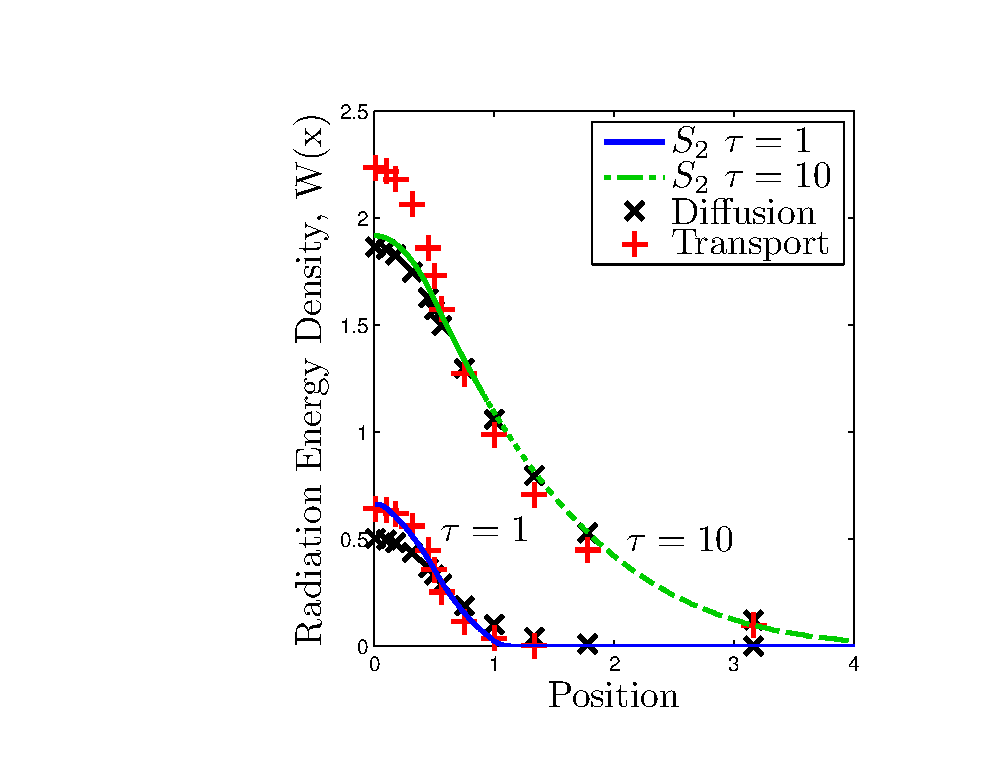
\includegraphics[width=5cm,trim=1.75in  0.5in 0.75in 0.5in,clip=true]{../chapter6_grey_radtran/Dissertation_Data/Su_Olson_S2_Radiation_Energy.pdf}
%\caption{$S_2$ radiation energy density profile for Su-Olson problem.}
%\label{fig:su_olson_s2_rad}
%\end{figure}
%\begin{figure}[!hbp]
%\centering
%\column{0.48\textwidth}
%\centering
%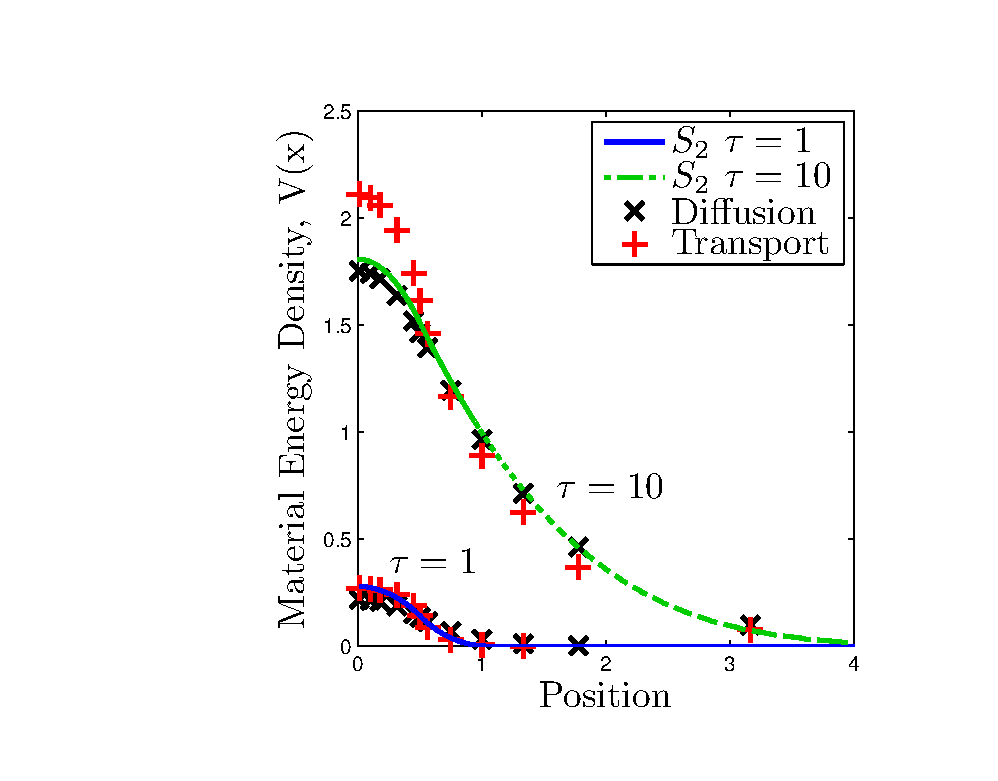
\includegraphics[width=5cm,trim=1.75in  0.5in 0.75in 0.5in,clip=true]{../chapter6_grey_radtran/Dissertation_Data/Su_Olson_S2_Material_Energy.pdf}
%\caption{$S_2$ material energy density profile for Su-Olson problem.}
%\label{fig:su_olson_s2_mat}
%\end{figure}
%\end{columns}
%Calculated using 200 cells, linear SLXS Lobatto, $\Delta t = 10^{-3}$
%\end{frame}

\begin{frame}
\frametitle{Su-Olson Results with $S_8$}
\begin{columns}[t]
\column{0.48\textwidth}
\centering
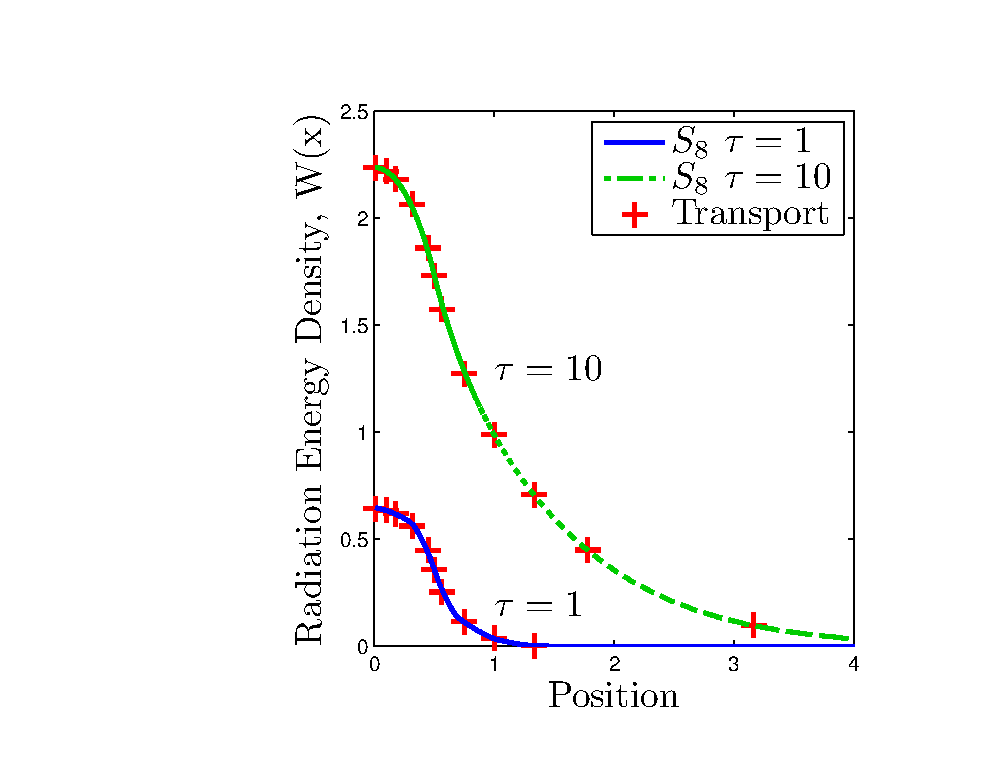
\includegraphics[width=5.5cm,trim=1.75in  0.5in 0.75in 0.5in,clip=true]{../chapter6_grey_radtran/Dissertation_Data/Su_Olson_S8_Radiation_Energy.pdf}
%\caption{$S_2$ radiation energy density profile for Su-Olson problem.}
%\label{fig:su_olson_s2_rad}
\column{0.48\textwidth}
\centering
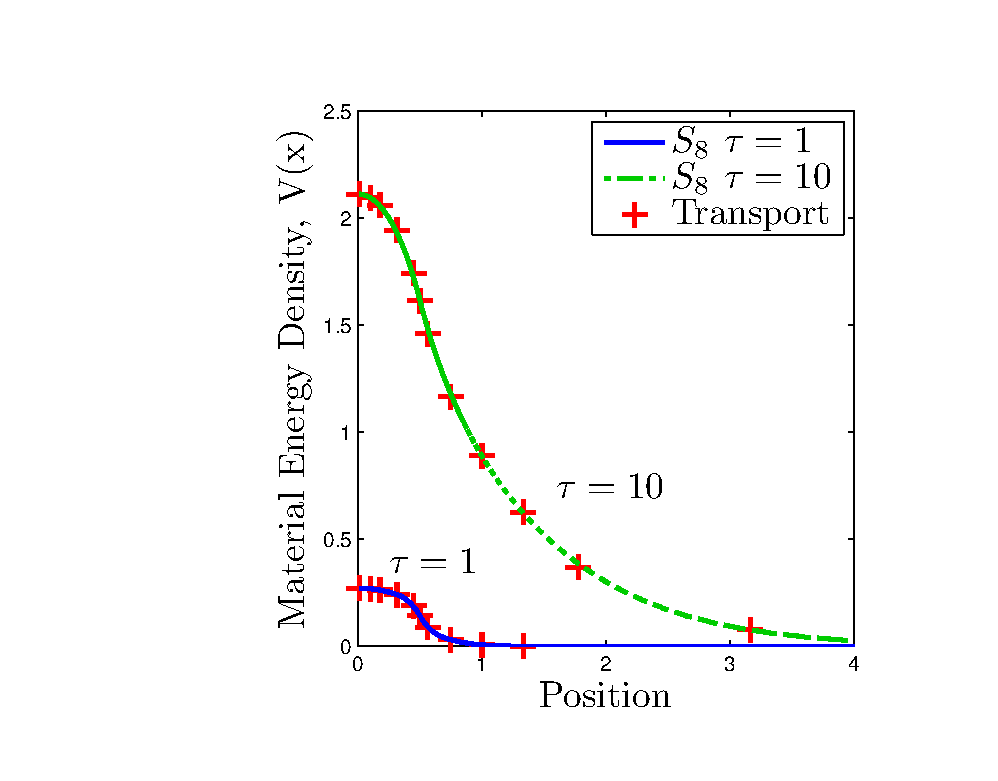
\includegraphics[width=5.5cm,trim=1.75in  0.5in 0.75in 0.5in,clip=true]{../chapter6_grey_radtran/Dissertation_Data/Su_Olson_S8_Material_Energy.pdf}
%\caption{$S_2$ material energy density profile for Su-Olson problem.}
\end{columns}
Calculated using 200 cells, linear SLXS Lobatto, $\Delta t = 10^{-3}$
\end{frame}

\subsection{MMS}

\begin{frame}
\frametitle{Error Measures}
\bea
E_{\phi} &=& \sqrt{\sum_{c=1}^{N_{cell}}{ \frac{\Delta x}{2} \sum_{q=1}^{N_{qf}}{ w_q \left(\widetilde{\phi}(s_q , t_{end}) - \phi(s_q,t_{end})  \right)^2 } } } \\
E_{\phi_A} &=& \sqrt{
\sum_{c=1}^{N_{cell}}{ 
\frac{\Delta x}{2} 
\left( 
\frac{1}{2}\sum_{q=1}^{N_{qf}}{ w_q \widetilde{\phi}(s_q , t_{end})}  - \frac{1}{2}\sum_{q=1}^{N_{qf}}{ w_q \phi(s_q , t_{end})} 
\right)^2 
} 
} 
\eea
\vspace{0.2in}
$E_T$ and $E_{T_A}$ are defined analogously.  $N_{qf} = 2P+ 7$, Gauss quadrature
\end{frame}

\begin{frame}
\frametitle{Choice of MMS}
Elect to use separable solution of the form
\beanum
I_d(x,\mu_d,t) &=& M(\mu_d) F(t) W_I(x) \\
T(x) &=& F(t) W_T(x) \\
\phi(x) &=& C_M F(t) W_I(x) \\
C_M &=& \sum_{d=1}^{N_{dir}} { w_d M(\mu_d) }
\eeanum
\end{frame}


\begin{frame}
\frametitle{SDIRK Order of Convergence}
\bea
M(\mu_d) &=& \frac{1}{4\pi} \\
W_I(x) &=& \frac{10}{4\pi} \\
W_T(x) &=&  10 \\
F(t) &=& 45 \cos\left( \pi t \right) + 46 \\
t &\in&[0,1] \\
\sigma_s &=& 0.1\\
\sigma_a &=& 2.5\\
C_v &=& 0.2 \\
x &\in & [0,10]
\eea
10 equally-spaced cells, quartic SLXS Gauss
\end{frame}

\begin{frame}
\frametitle{SDIRK Order of Convergence}
\begin{columns}[t]
\column{0.5\textwidth}
\centering
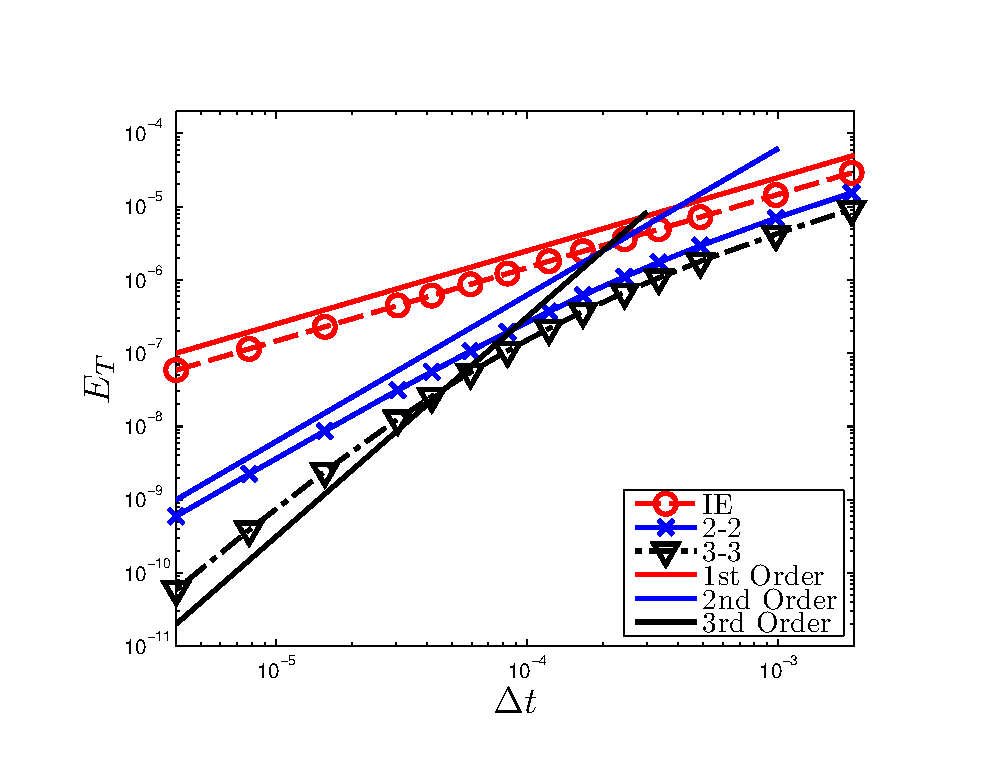
\includegraphics[width=\textwidth,trim=0.25in  0.2in 0.75in 0.5in,clip=true]{../chapter6_grey_radtran/Dissertation_Data/Time_Integrators_Convergence_Temperature.pdf}
\column{0.5\textwidth}
\centering
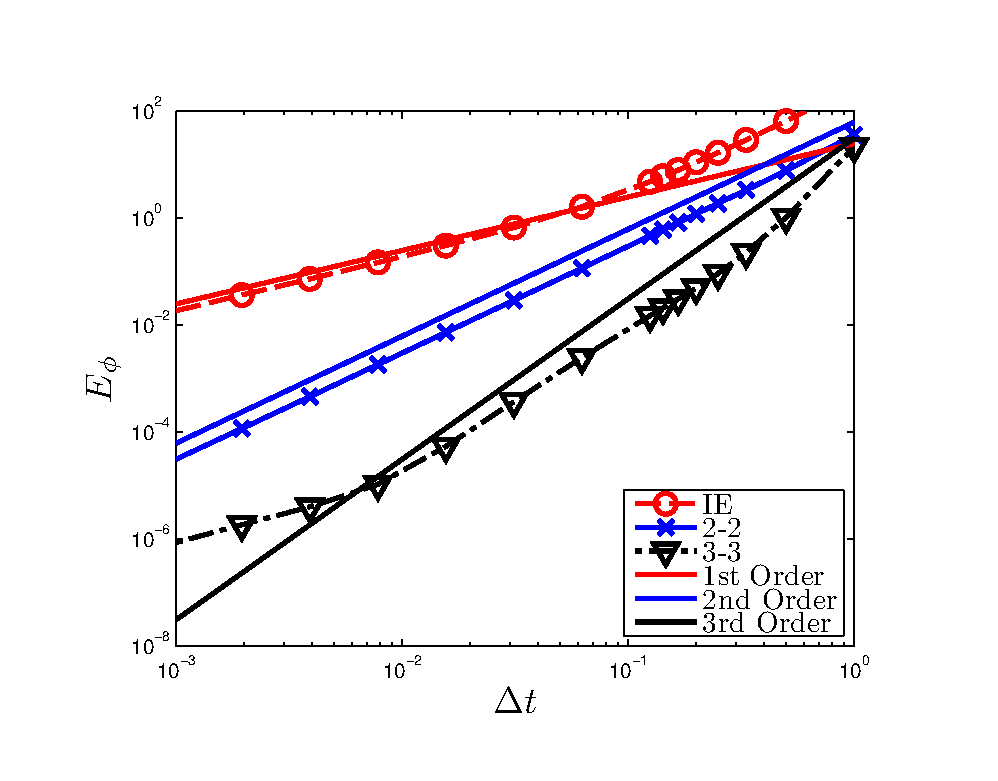
\includegraphics[width=\textwidth,trim=0.25in  0.2in 0.75in 0.5in,clip=true]{../chapter6_grey_radtran/Dissertation_Data/Time_Integrators_Convergence_Phi.pdf}
\end{columns}
\end{frame}


\subsection{MMS2}
\begin{frame}
\frametitle{Variable Material Properties Problem- MMS2}
\bea
M(\mu_d) &=& \frac{1}{4\pi} \\
W_I(x) &=& 9 \cos\left( \frac{\pi x}{10} - \frac{\pi}{2} \right) + 3  \\
W_T(x) &=&  5 \cos\left( \frac{\pi x}{10} - \frac{\pi}{2} \right) + 5 \\
F(t) &=&  1 + .02t \\
C_v &=& 0.2 + 0.01 T^3 \\
\sigma_a &=& \frac{10^4}{T^3} \\
\sigma_s &=& 0.5 
\eea
3-3 Alexander, $\Delta t = 10^{-3}$
\end{frame}

\begin{frame}
\frametitle{Must Account for Spatially Varying Material Properties}
SL Gauss, $P\in[1,4]$.  Limited $L^2$ convergence.
\begin{columns}[t]
\column{0.5\textwidth}
\centering
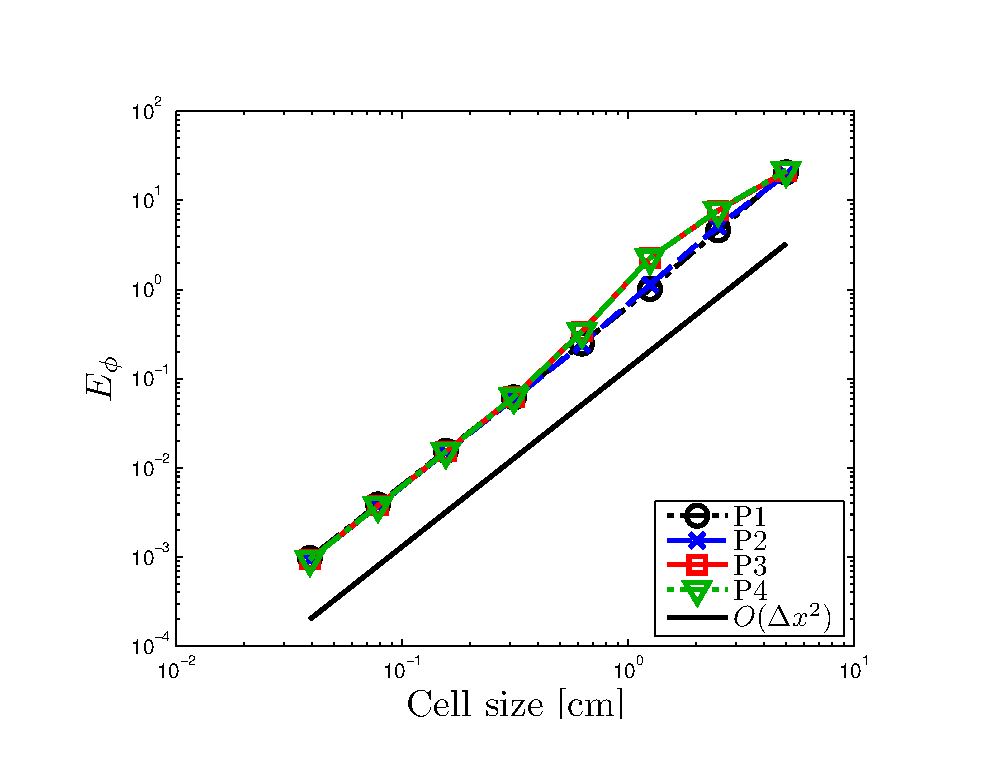
\includegraphics[width=\textwidth,trim=0.25in  0.2in 0.75in 0.5in,clip=true]{../chapter6_grey_radtran/Dissertation_Data/MMS3_Constant_XS_SL_Gauss_phi_L2.pdf}
\column{0.5\textwidth}
\centering
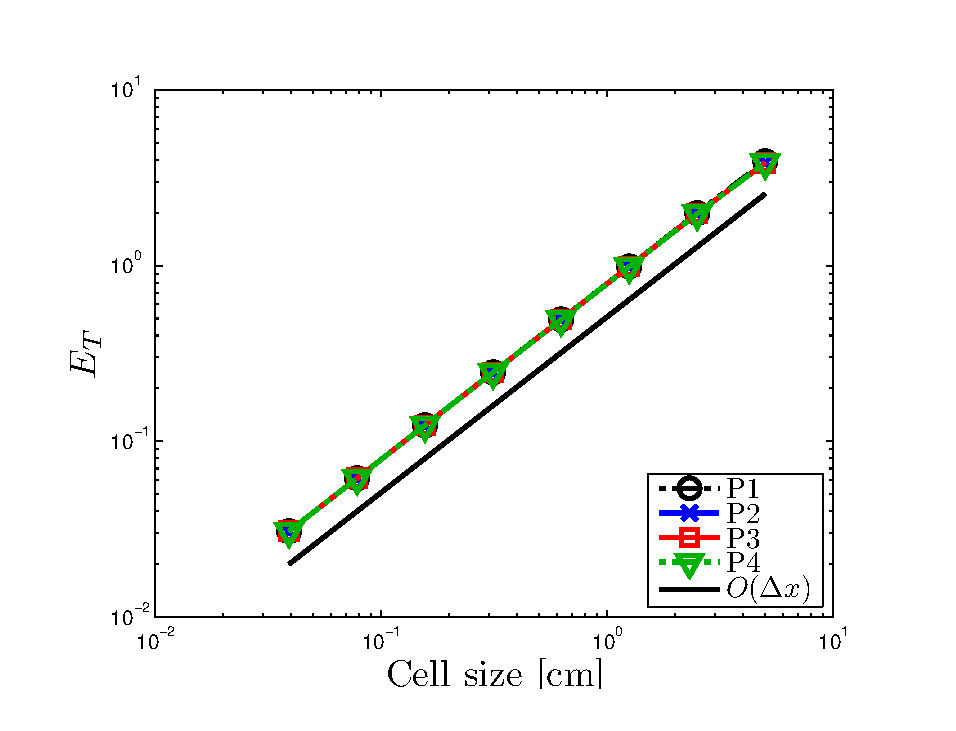
\includegraphics[width=\textwidth,trim=0.25in  0.2in 0.75in 0.5in,clip=true]{../chapter6_grey_radtran/Dissertation_Data/MMS3_Constant_XS_SL_Gauss_temp_L2.pdf}
\end{columns}
\end{frame}

\begin{frame}
\frametitle{This Is Not a Pure Absorber Test Problem}
SL Gauss, $P\in[1,4]$.  
\begin{columns}[t]
\column{0.5\textwidth}
\centering
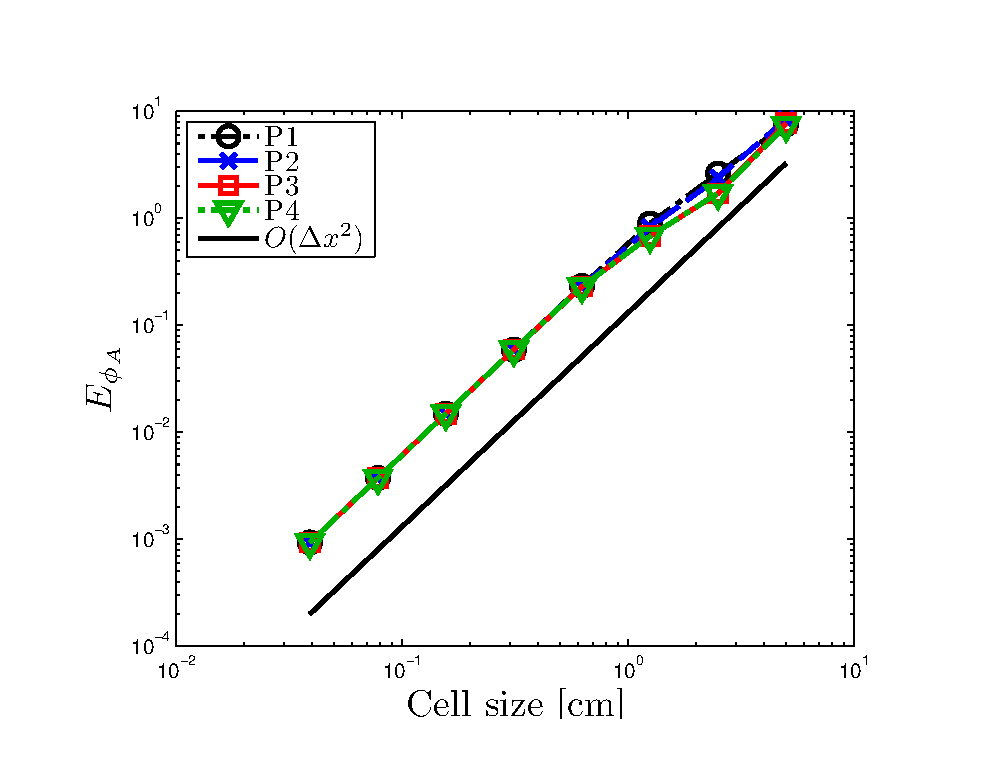
\includegraphics[width=\textwidth,trim=0.25in  0.2in 0.75in 0.5in,clip=true]{../chapter6_grey_radtran/Dissertation_Data/MMS3_Constant_XS_SL_Gauss_phi_A.pdf}
\column{0.5\textwidth}
\centering
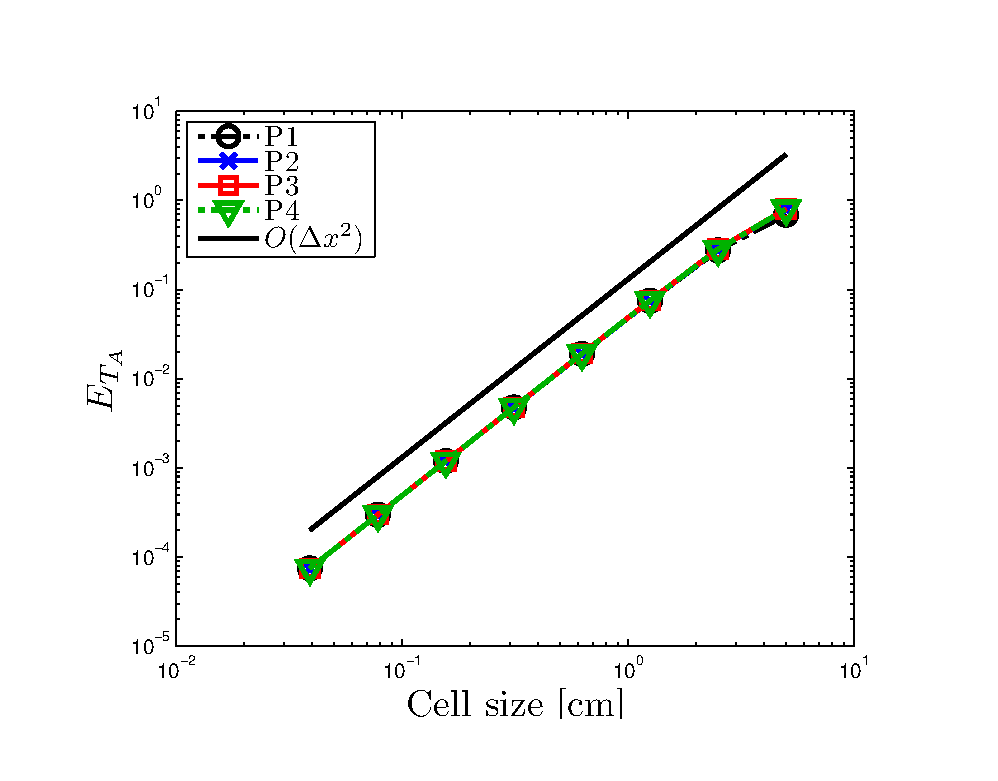
\includegraphics[width=\textwidth,trim=0.25in  0.2in 0.75in 0.5in,clip=true]{../chapter6_grey_radtran/Dissertation_Data/MMS3_Constant_XS_SL_Gauss_temp_A.pdf}
\end{columns}
In a neutron transport pure absorber test problem, cell-wise constant cross section assumption yields poor $L^2$ convergence, but very accurate cell average interaction rates. 
\end{frame}

\begin{frame}
\frametitle{SLXS $E_{\phi}$ Convergence}
\begin{columns}[t]
\column{0.5\textwidth}
\centering
SLXS Lobatto
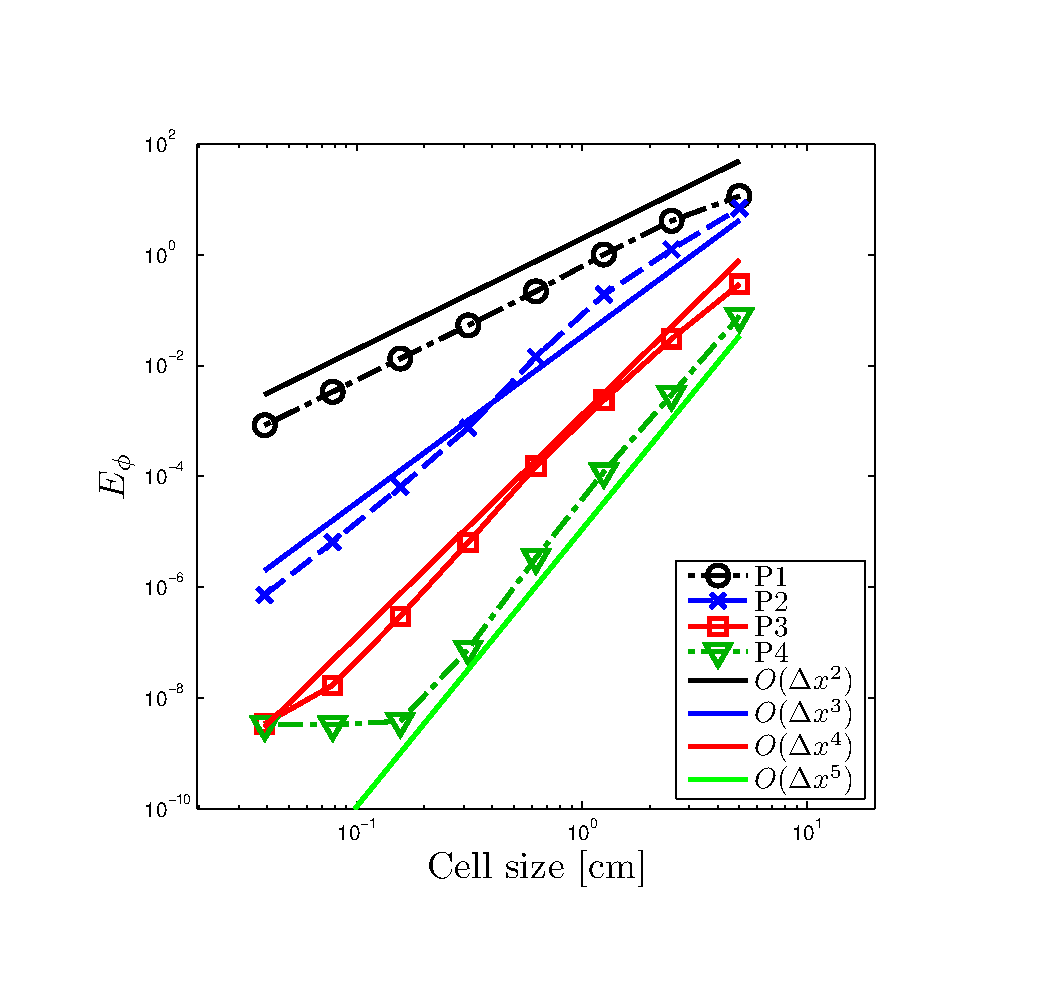
\includegraphics[width=\textwidth,trim=0.25in  0.2in 0.75in 0.5in,clip=true]{../chapter6_grey_radtran/Dissertation_Data/MMS3_SLXS_Lobatto_phi_L2.pdf}
\\
$\propto P+1$
\column{0.5\textwidth}
\centering
SLXS Gauss
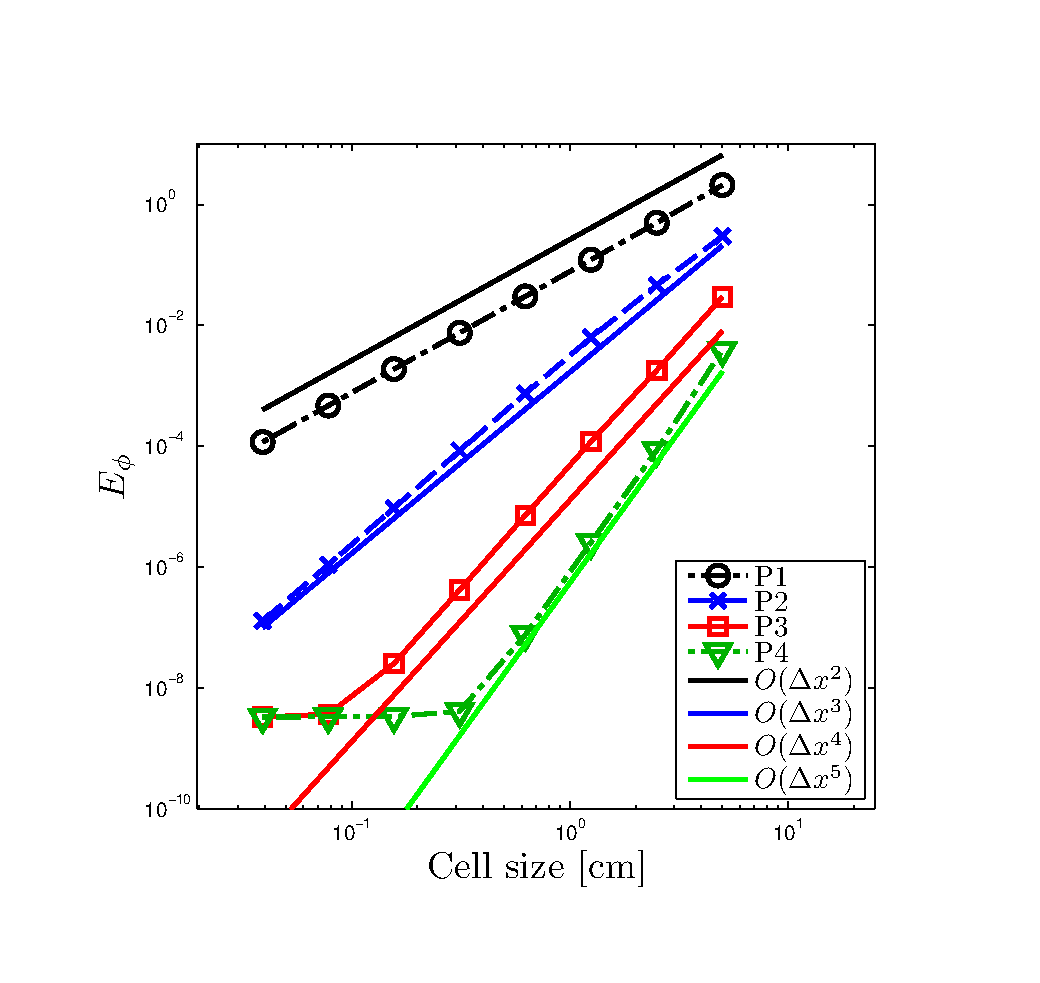
\includegraphics[width=\textwidth,trim=0.25in  0.2in 0.75in 0.5in,clip=true]{../chapter6_grey_radtran/Dissertation_Data/MMS3_SLXS_Gauss_phi_L2.pdf}
\\
$\propto P+1$
\end{columns}
\end{frame}

\begin{frame}
\frametitle{Plateauing of Errors}
Caused by point-wise relative change convergence criteria.  For temperature:
\bea
\text{err\_t} &=& \max_{c=1}^{N_{cells}} \left[ ~\max_{j=1}^{N_P} \left[  ~\abs{ \frac{ \Delta T_j }{ T_{j,*} } } ~\right] ~\right] \\
\text{converged} &=& \text{err\_t} < \epsilon_T
\eea
All MMS results generated with $\epsilon_T = 10^{-11},~\epsilon_{\phi}=10^{-13}$. 
\end{frame}

\begin{frame}
\frametitle{Looser Tolerances}
SLXS Gauss $E_{\phi}$ convergence if ...
\vspace{0.1in}
\begin{columns}[t]
\column{0.5\textwidth}
\centering
$\epsilon_T = 10^{-8},~\epsilon_{\phi}=10^{-10}$
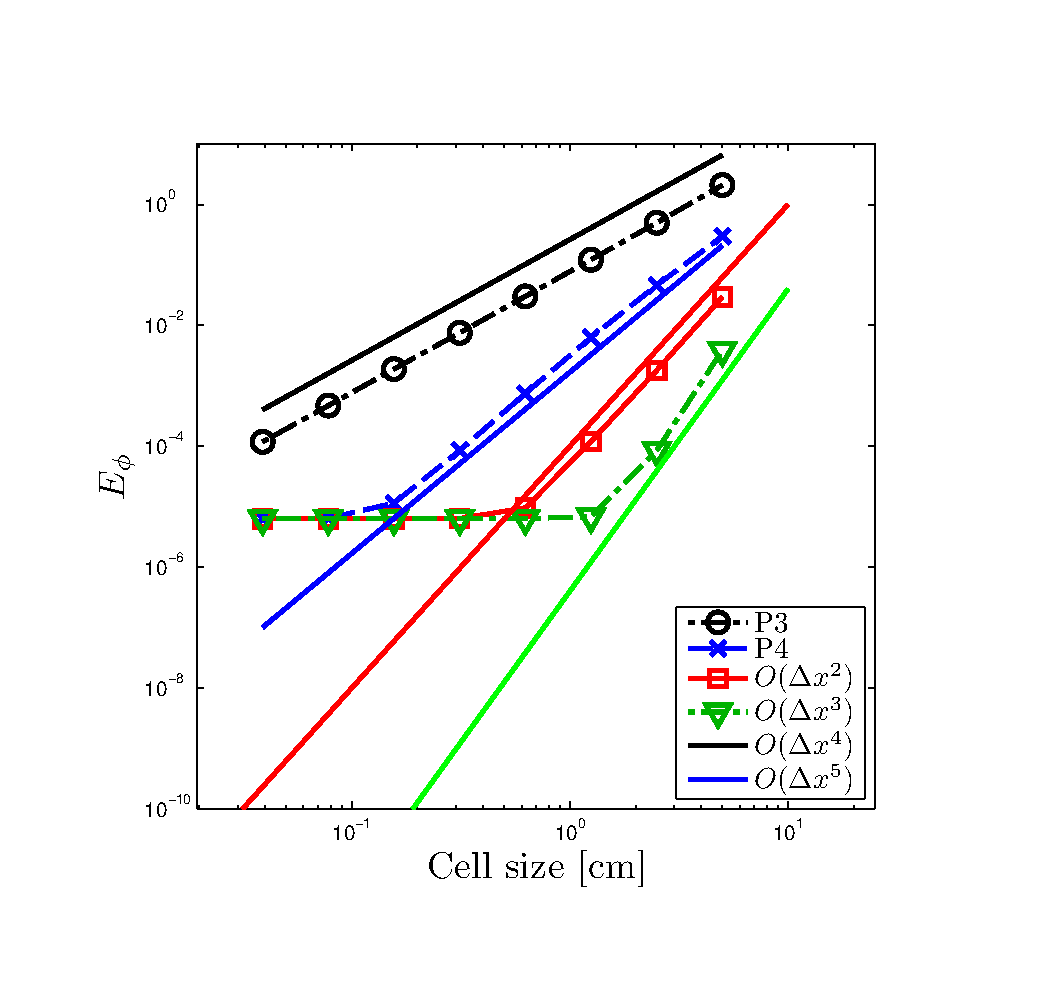
\includegraphics[width=\textwidth,trim=0.25in  0.2in 0.75in 0.5in,clip=true]{../chapter6_grey_radtran/Dissertation_Data/MMS3_Low_Tol_First_SLXS_Gauss_phi_L2.pdf}
\column{0.5\textwidth}
\centering
$\epsilon_T = 10^{-11},~\epsilon_{\phi}=10^{-13}$
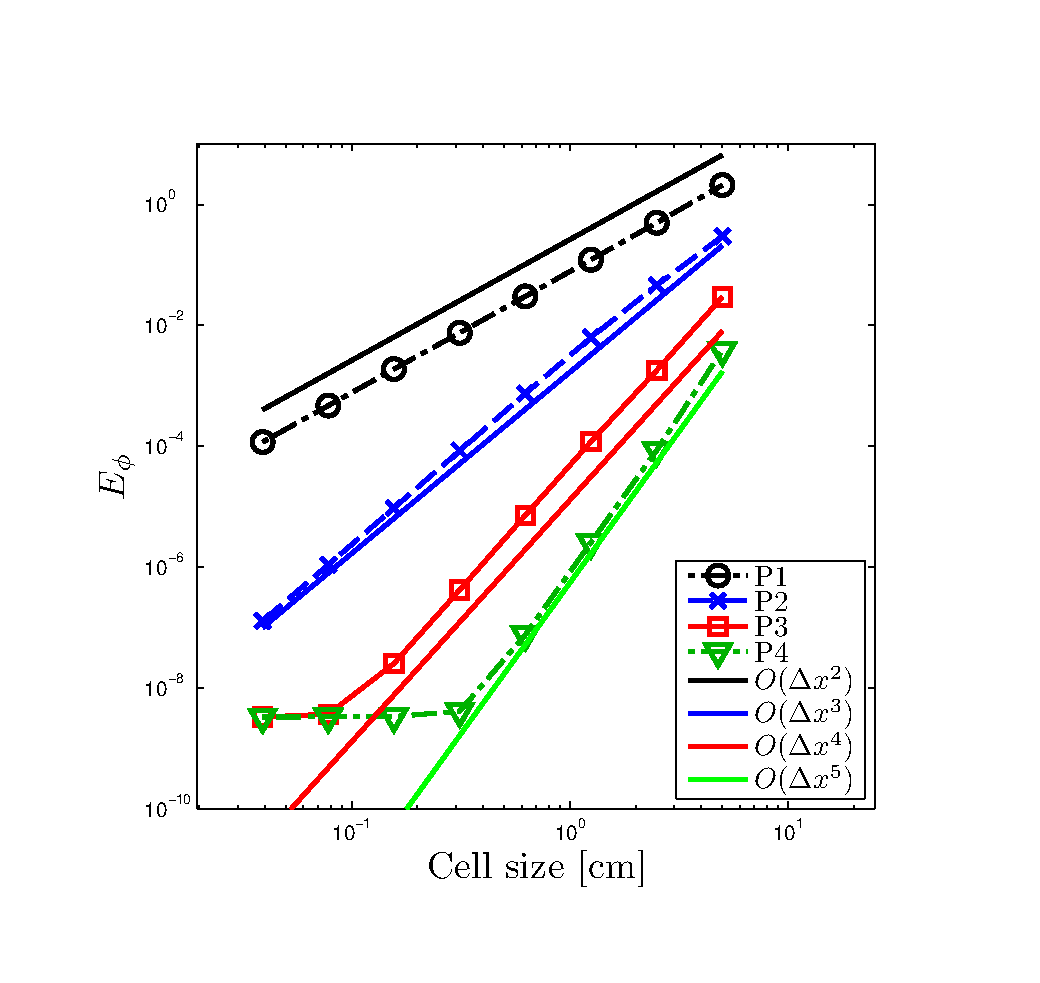
\includegraphics[width=\textwidth,trim=0.25in  0.2in 0.75in 0.5in,clip=true]{../chapter6_grey_radtran/Dissertation_Data/MMS3_SLXS_Gauss_phi_L2.pdf}
\end{columns}
\end{frame}

\begin{frame}
\frametitle{SLXS $E_T$ Convergence}
\begin{columns}[t]
\column{0.5\textwidth}
\centering
SLXS Lobatto
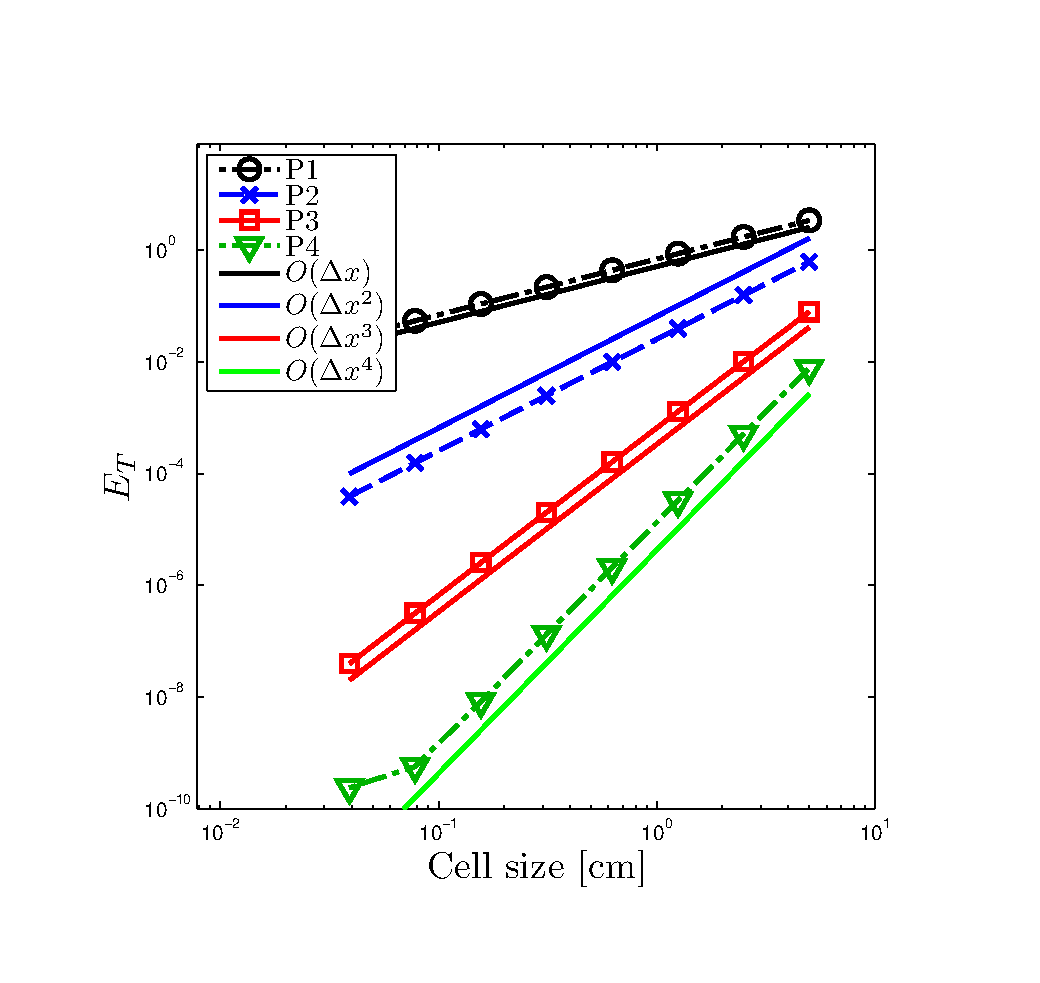
\includegraphics[width=\textwidth,trim=0.25in  0.2in 0.75in 0.5in,clip=true]{../chapter6_grey_radtran/Dissertation_Data/MMS3_SLXS_Lobatto_temp_L2.pdf}
\\
$\propto P$
\column{0.5\textwidth}
\centering
SLXS Gauss
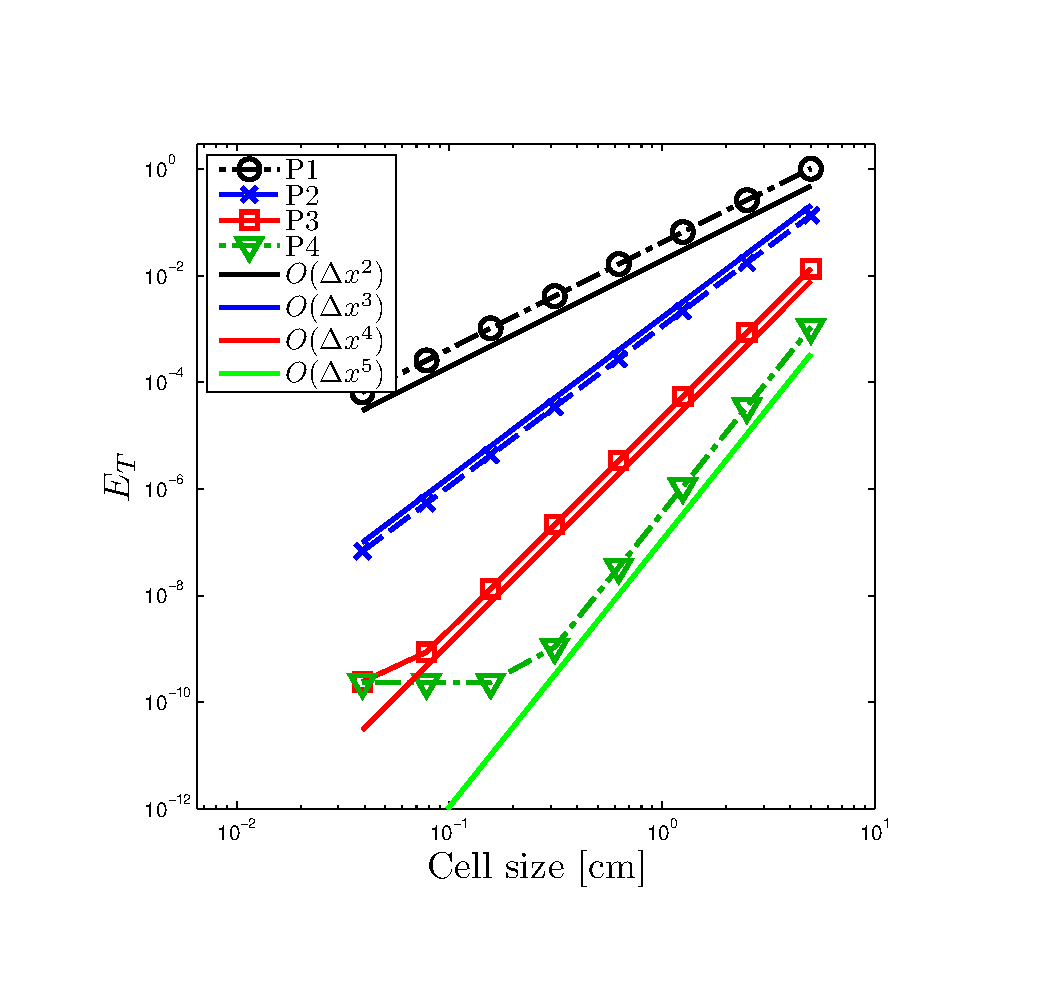
\includegraphics[width=\textwidth,trim=0.25in  0.2in 0.75in 0.5in,clip=true]{../chapter6_grey_radtran/Dissertation_Data/MMS3_SLXS_Gauss_temp_L2.pdf}
\\
$\propto P+1$
\end{columns}
\end{frame}

\subsection{Marhsak Wave}
\begin{frame}
\frametitle{Marshak Wave Problem}
Unit current incident intensity on left face.  Vacuum right boundary condition.  Initially cold slab.  No analytic solution.
\bea
a&=&c=C_v = 1 \\
x&\in&[0,1] \\
t&\in&[0,1]  \\
T_0^4& =& 1E-5 \\
\sigma_s &=& 0 \\
\sigma_a &=& \frac{1}{T^3}
\eea
\end{frame}

\begin{frame}
\frametitle{Blading with Cell-Wise Constant Assumption}
Linear TL, volumetric average opacity
\begin{columns}[t]
\column{0.5\textwidth}
\centering
Radiation energy density
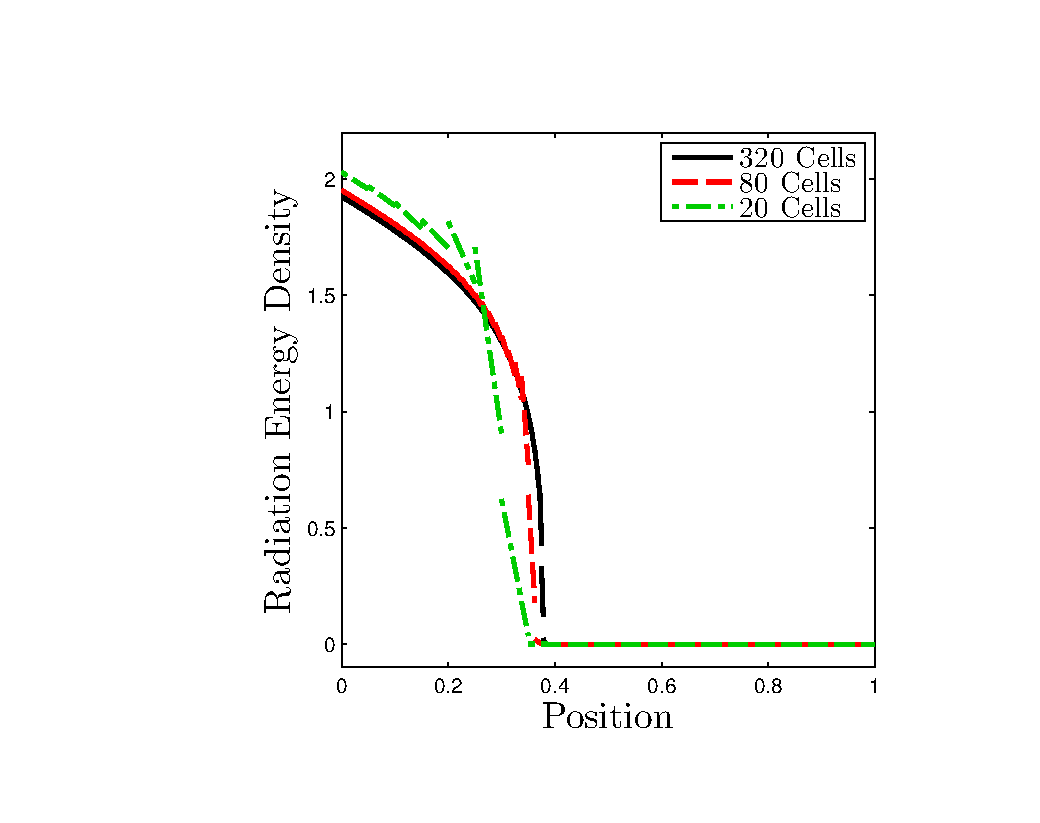
\includegraphics[width=\textwidth,trim=1.2in  0.2in 0.75in 0.5in,clip=true]{../chapter6_grey_radtran/Dissertation_Data/Reorder_Blading_Radiation_Full_MultiCell.pdf}
\column{0.5\textwidth}
\centering
Material temperature
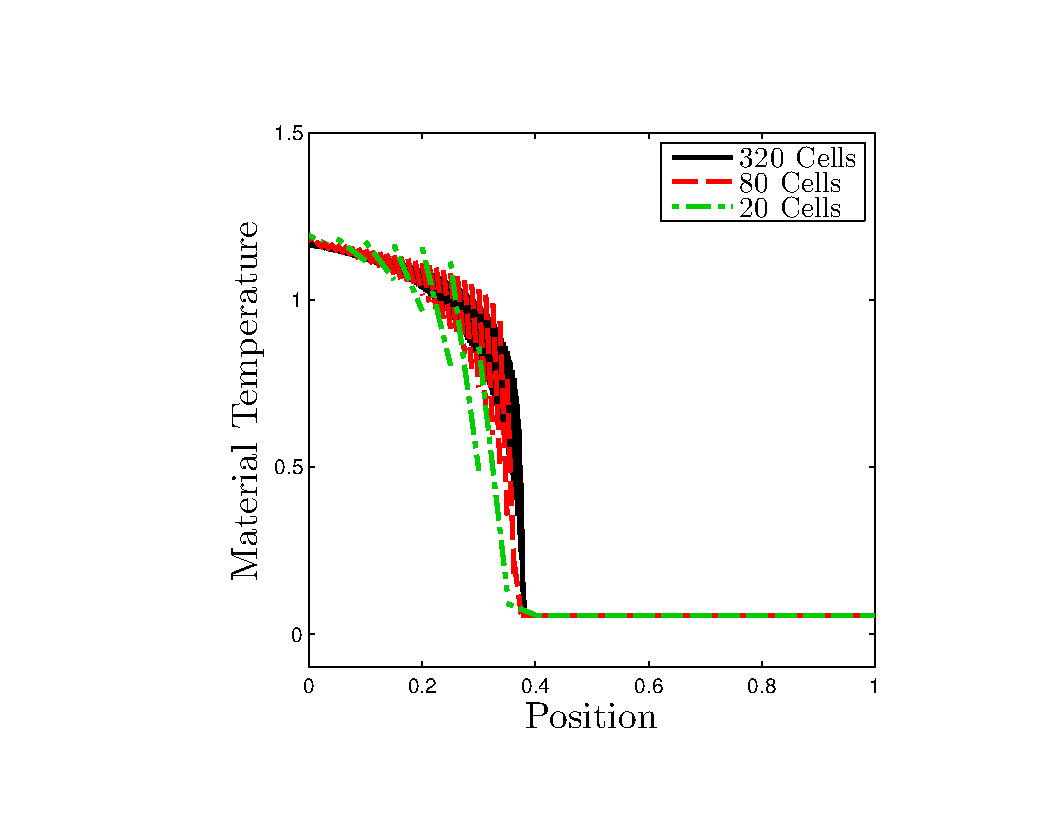
\includegraphics[width=\textwidth,trim=1.2in  0.2in 0.75in 0.5in,clip=true]{../chapter6_grey_radtran/Dissertation_Data/Reorder_Blading_Temperature_Full_MultiCell.pdf}
\end{columns}
\end{frame}

\begin{frame}
\frametitle{SLXS Treatment}
Linear SLXS Lobatto
\begin{columns}[t]
\column{0.5\textwidth}
\centering
Radiation energy density
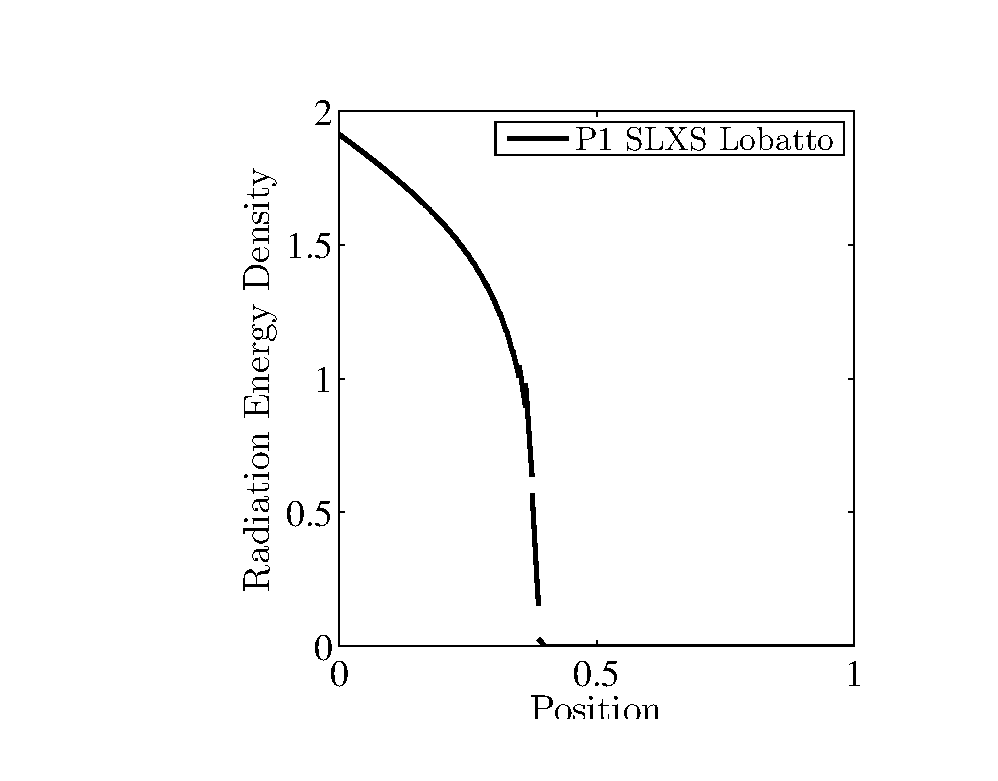
\includegraphics[width=\textwidth,trim=1.2in  0.2in 0.75in 0.5in,clip=true]{../chapter6_grey_radtran/Dissertation_Data/SLXS_Lobatto_80_Cells_Radiation.pdf}
\column{0.5\textwidth}
\centering
Material temperature
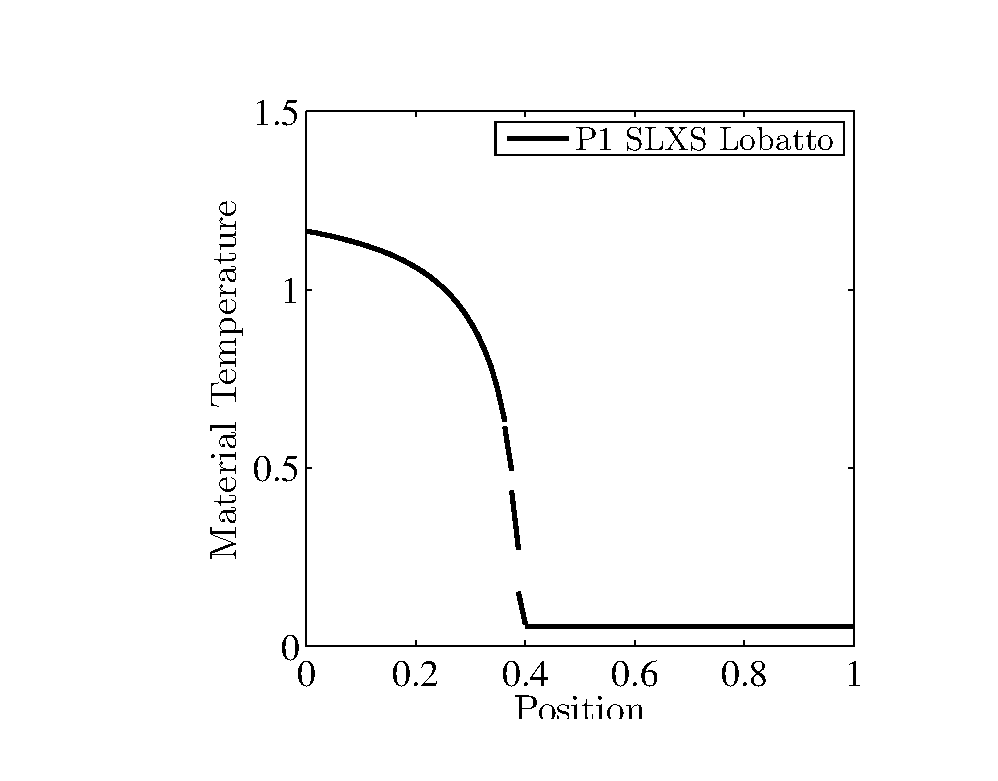
\includegraphics[width=\textwidth,trim=1.2in  0.2in 0.75in 0.5in,clip=true]{../chapter6_grey_radtran/Dissertation_Data/SLXS_Lobatto_80_Cells_Temperature.pdf}
\end{columns}
\end{frame}

\begin{frame}
\frametitle{Time Resolution Cannot Be Neglected}
\centering
Quartic SLXS Lobatto, 1280 mesh cells, 2-2 SDIRK, $\Delta t = 0.01$
\\
\vspace{0.1in}
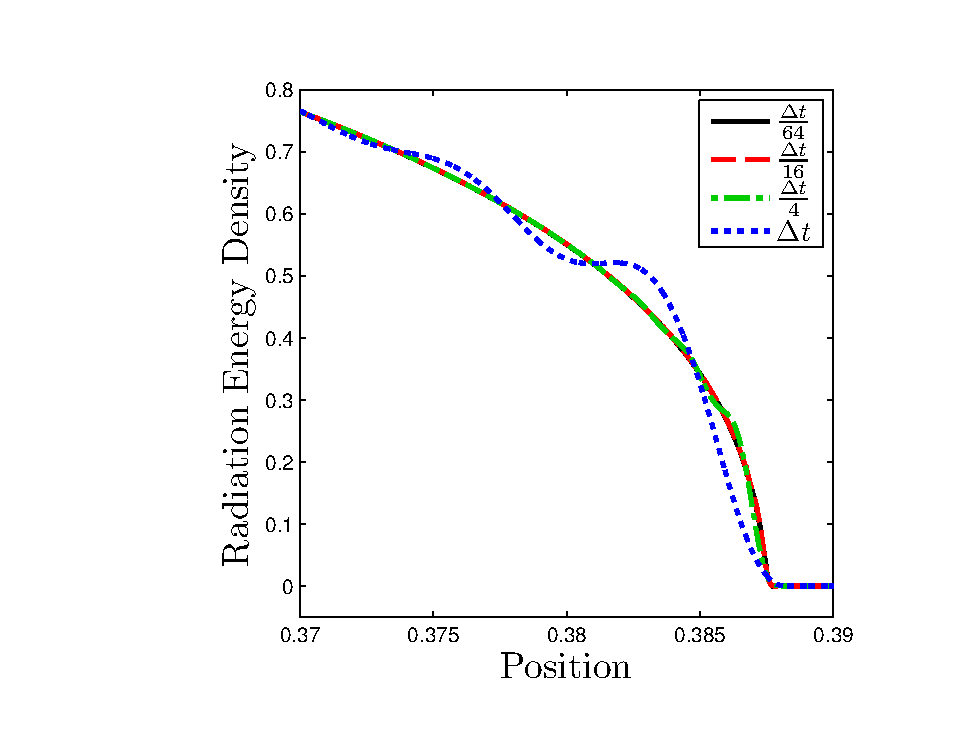
\includegraphics[width=0.9\textheight,trim=1.0in  0.2in 0.5in 0.5in,clip=true]{../chapter6_grey_radtran/Dissertation_Data/Time_Refinement_Zoom_Radiation.pdf}
\end{frame}


\begin{frame}
\frametitle{Extreme Zoom of $S_2$ Radiation Energy Density}
\begin{columns}[t]
\column{0.7\textwidth}
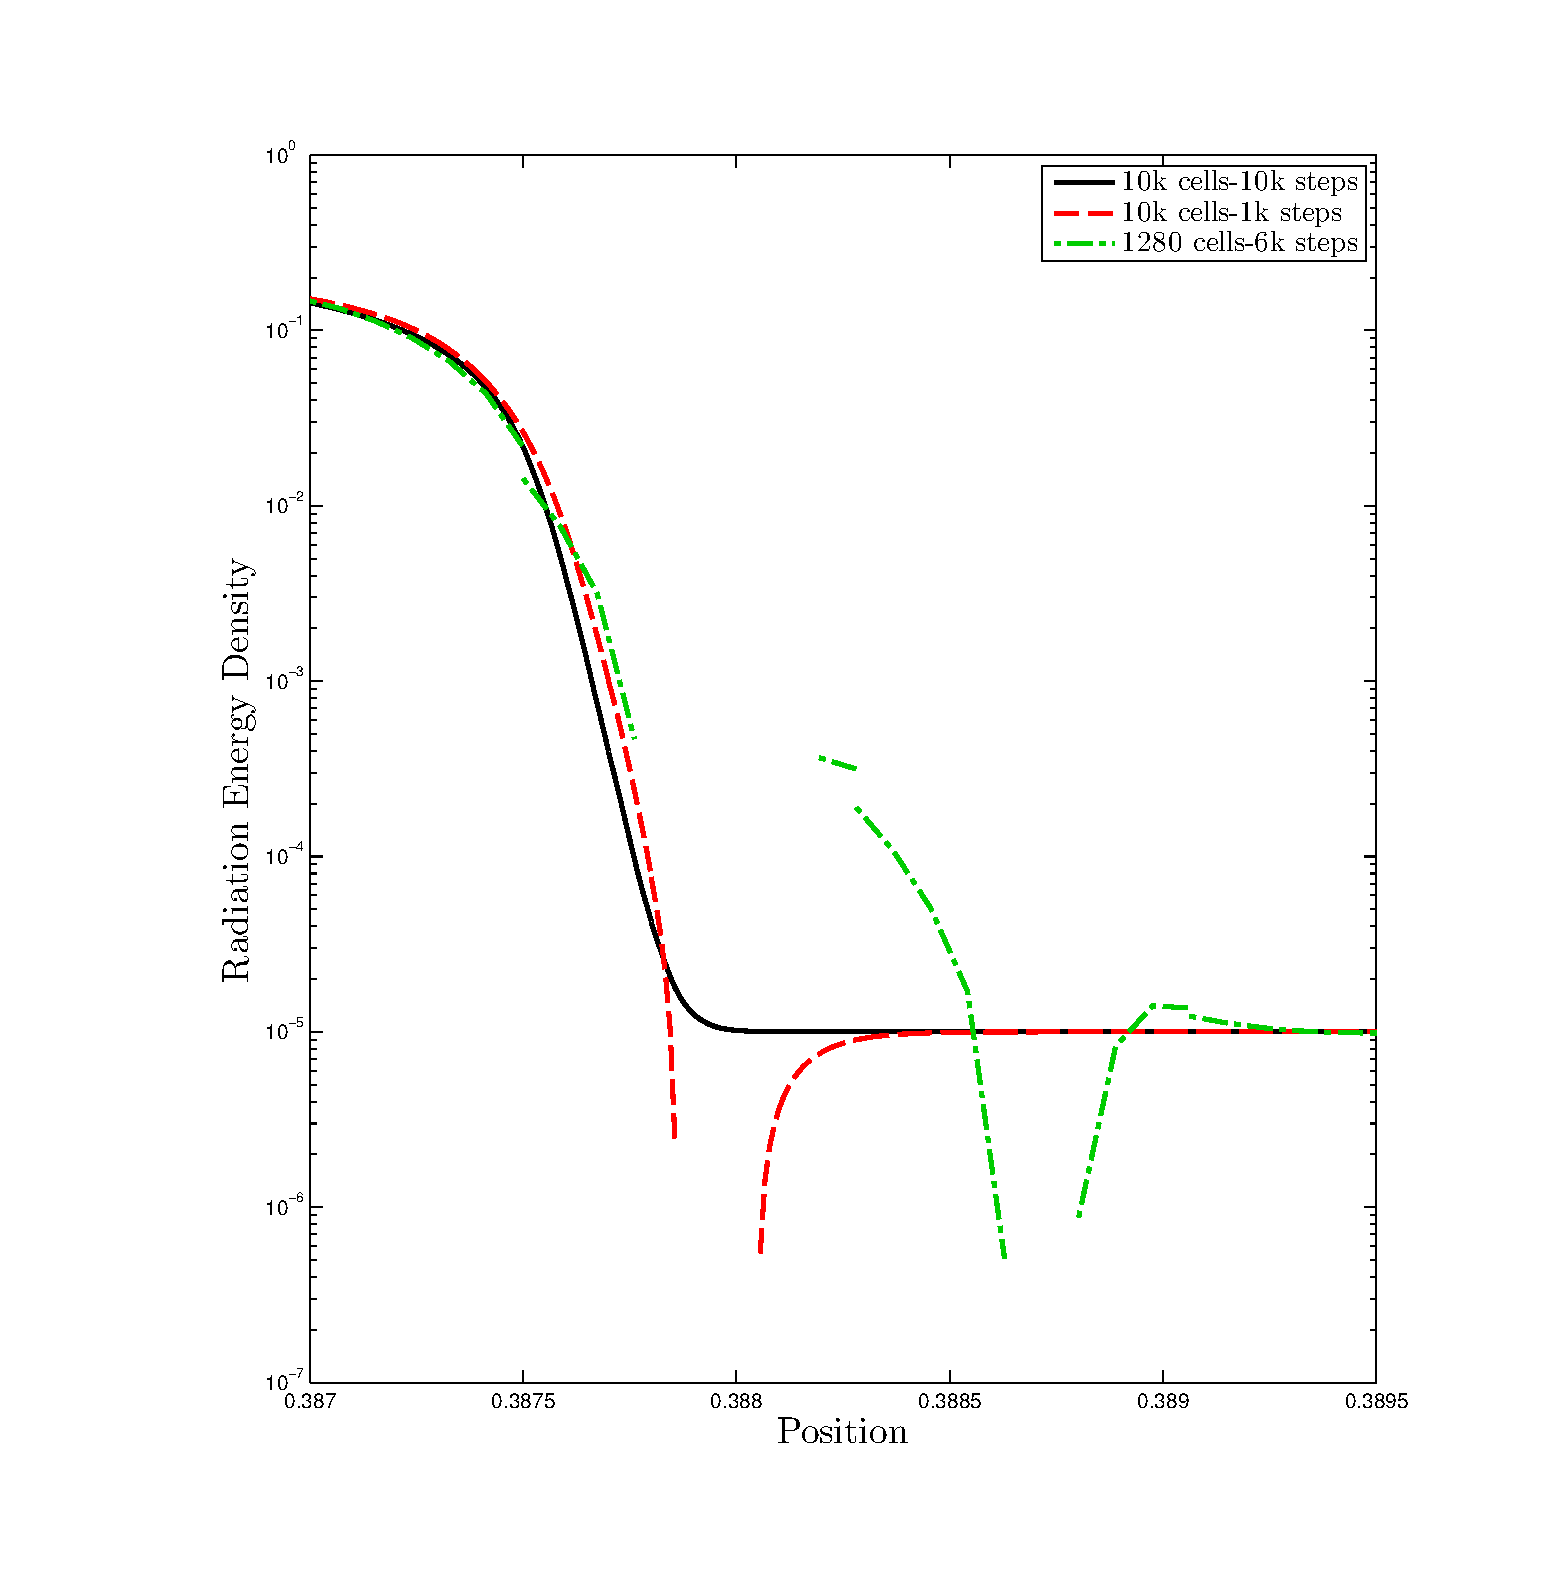
\includegraphics[height=0.8\textheight,trim=1.0in  0.75in 1.0in 1.0in,clip=true]{../chapter6_grey_radtran/Dissertation_Data/Zoom_10k_Phi.pdf}
\column{0.3\textwidth}
\begin{itemize}
\item Log scaly $y$-axis
\item Gaps caused by negative radiation energy densities
\end{itemize}
\end{columns}
\end{frame}

\begin{frame}
\frametitle{$S_2$ vs $S_8$}
\begin{columns}[t]
\column{0.5\textwidth}
\centering
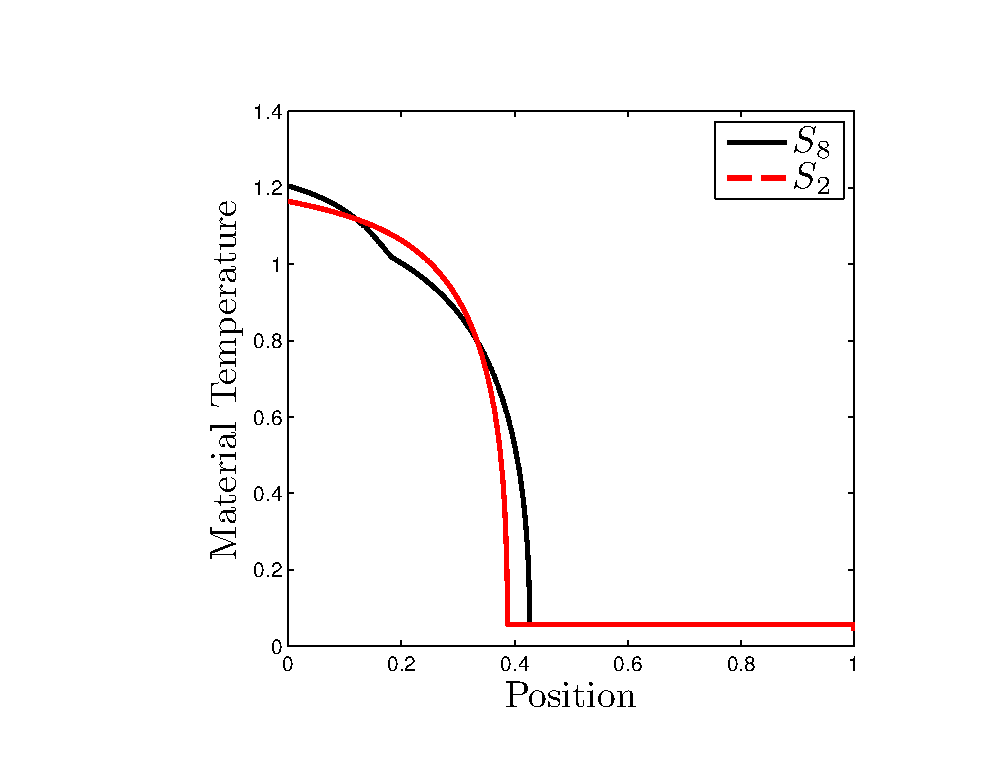
\includegraphics[width=2.5in,trim=1.0in  0.5in 0.2in 0.6in,clip=true]{../chapter6_grey_radtran/S8_vs_S2_Material_Temperature.pdf}
\column{0.5\textwidth}
\centering
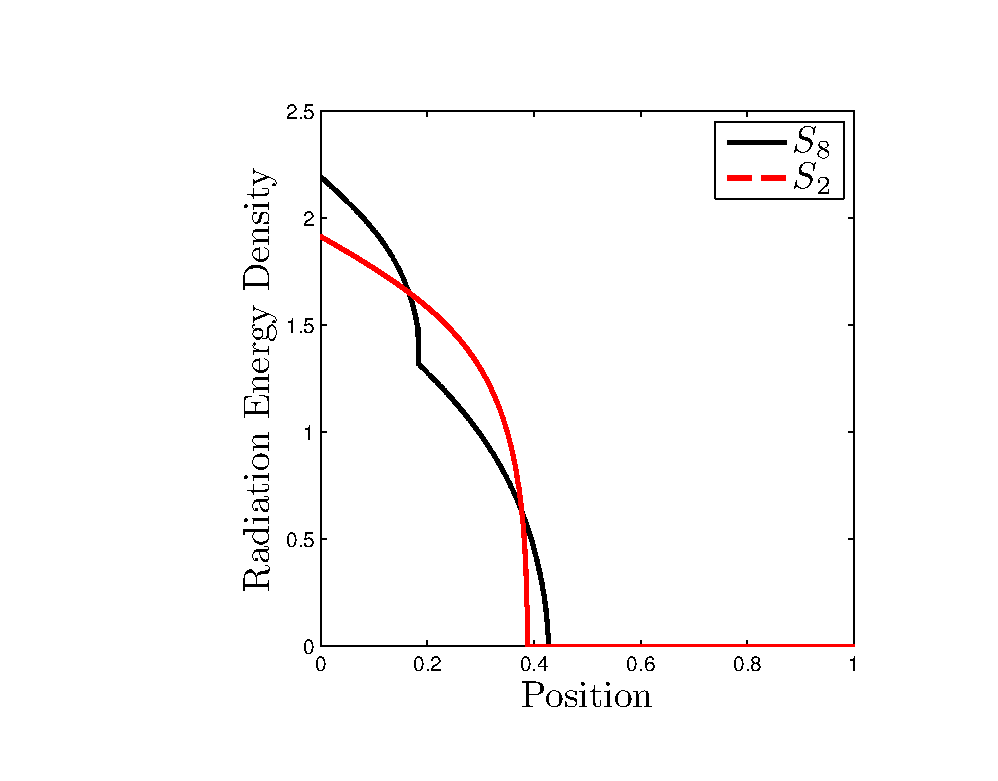
\includegraphics[width=2.5in,trim=1.0in  0.3in 0.2in 0.5in,clip=true]{../chapter6_grey_radtran/S8_vs_S2_Radiation_Energy_Density.pdf}
\end{columns}
\centering
5000 mesh cells, P4 SLXS Gauss, 5k time steps, 2-2 scheme
\end{frame}

\begin{frame}
\frametitle{$S_8$ Angular Intensity}
\centering
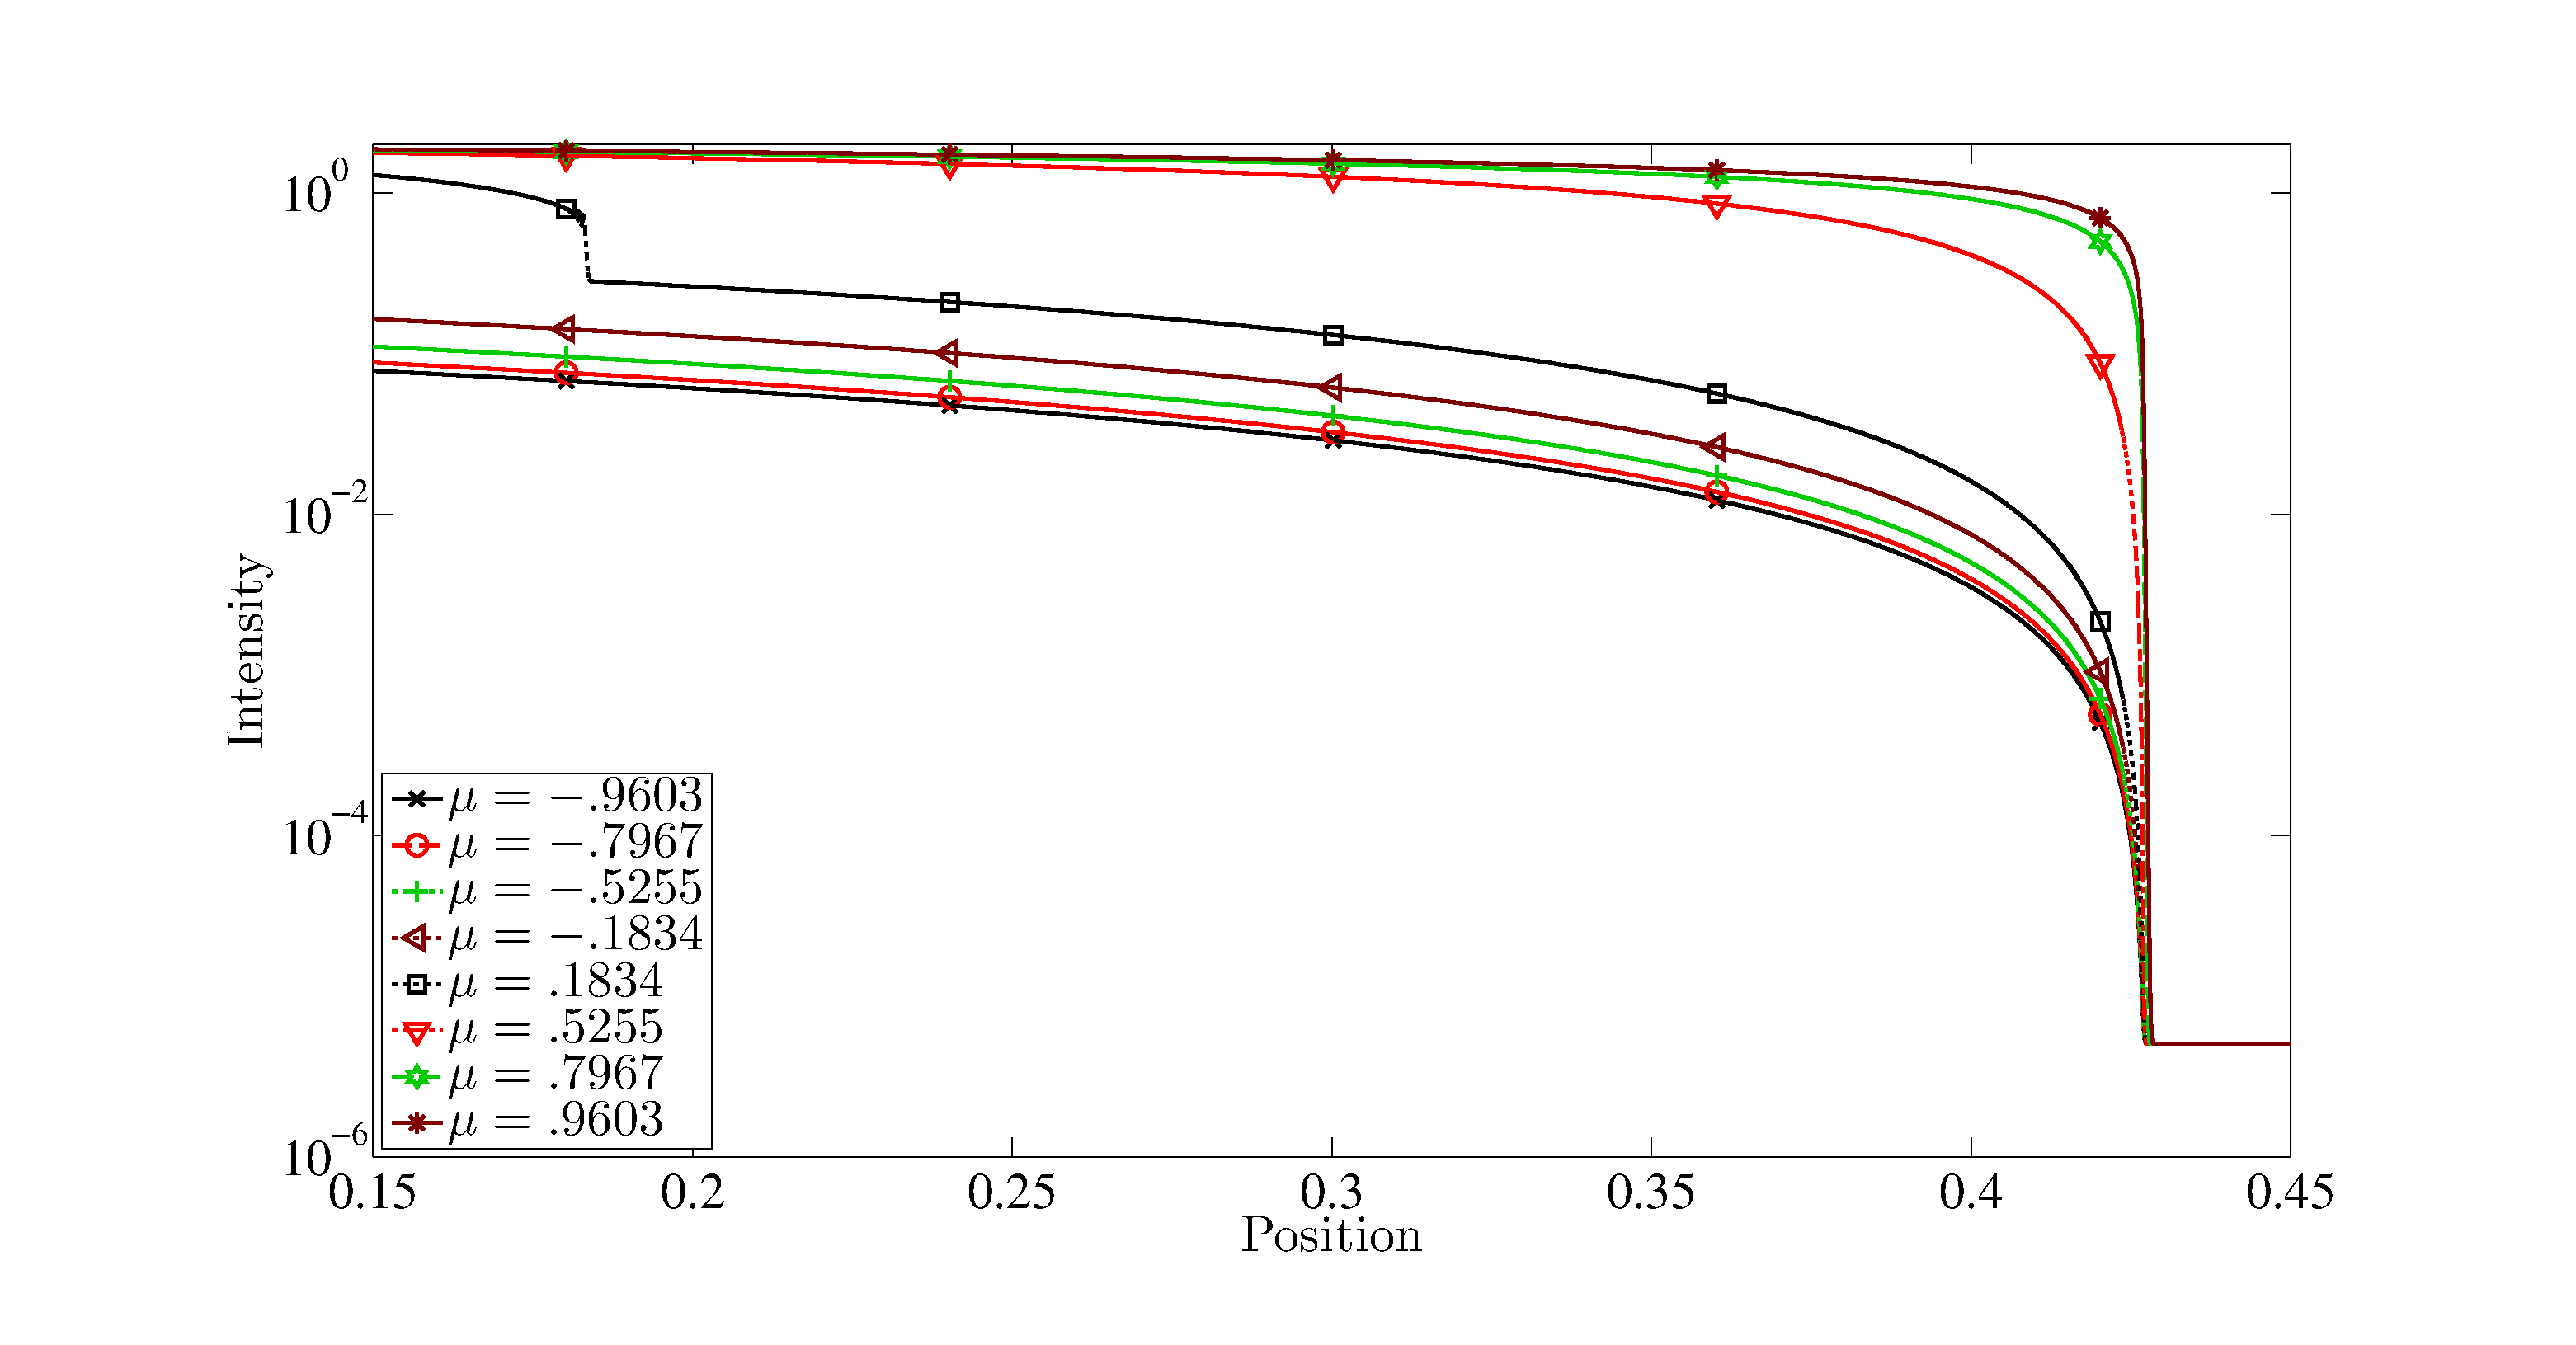
\includegraphics[width=\textwidth,trim=1.5in  0.5in 1.0in 1in,clip=true]{../chapter6_grey_radtran/S8_Intensity_SemiLogy.pdf}
\end{frame}

\begin{frame}
\frametitle{Wavefront Boundary Layers}
\centering
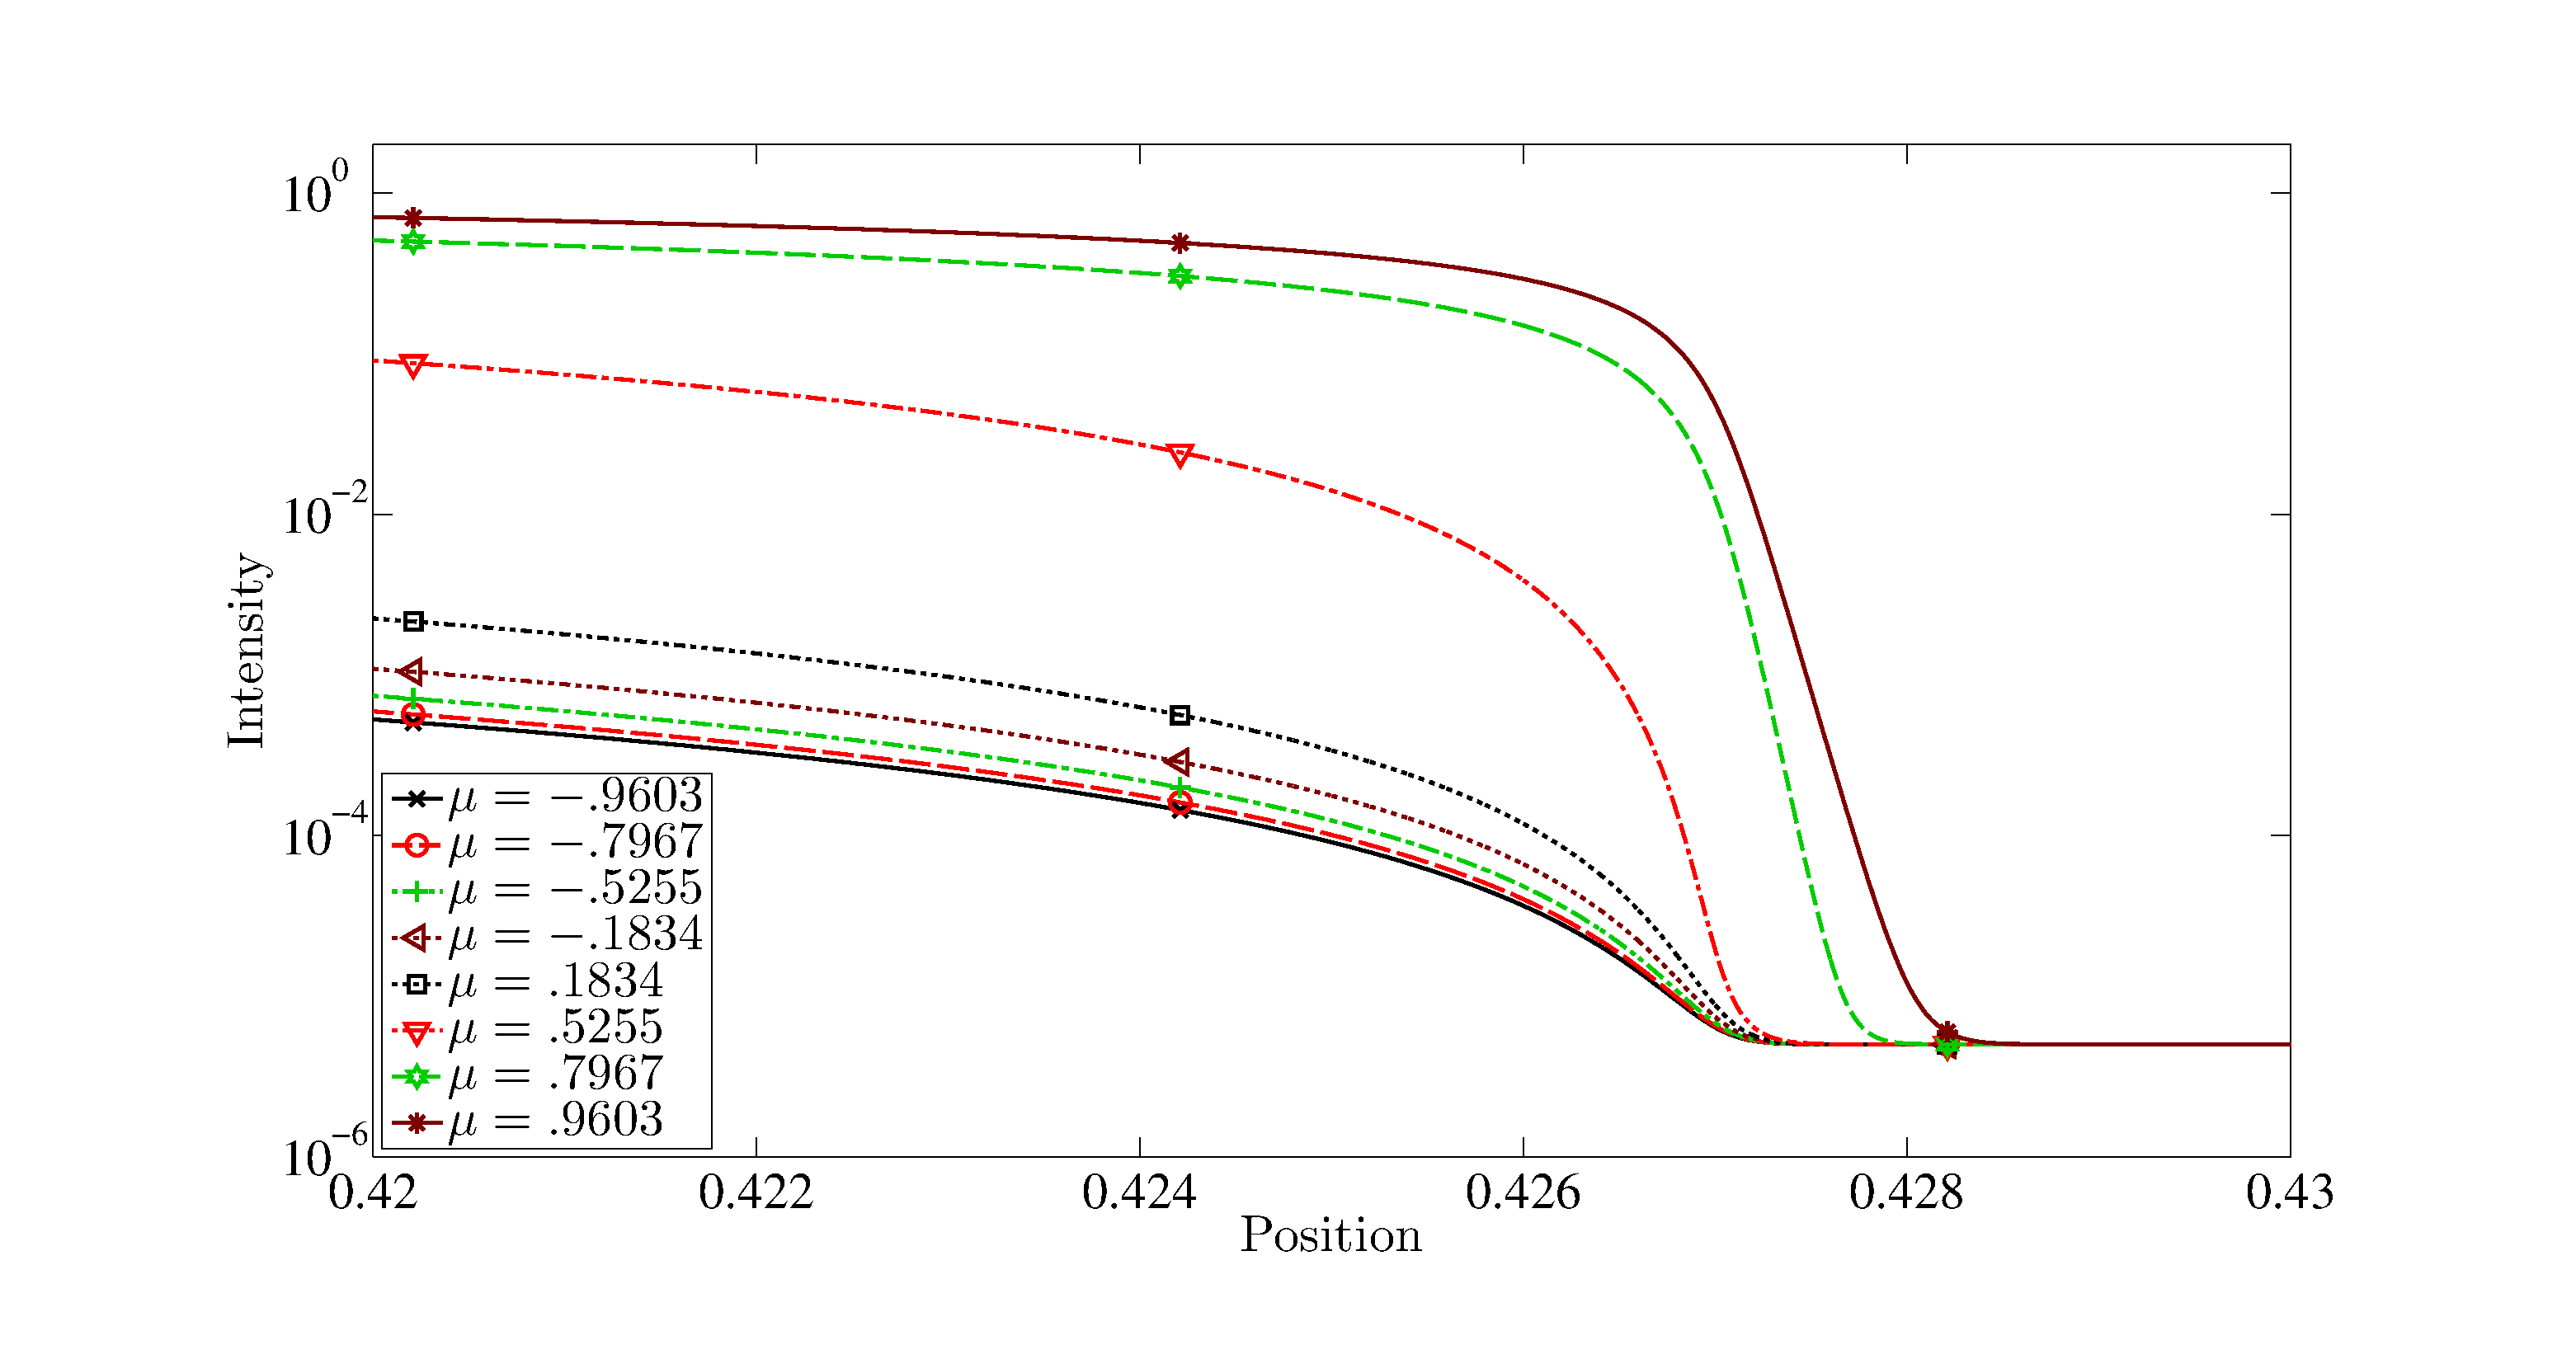
\includegraphics[width=1.05\textwidth,trim=1.75in  0.2in 1in 0.75in,clip=true]{../chapter6_grey_radtran/Dissertation_Data/S8_thermal_wavefront_boundary_layer.pdf}
\end{frame}

\begin{frame}
\frametitle{Need More Resolution for Interior Boundary Layer}
\centering
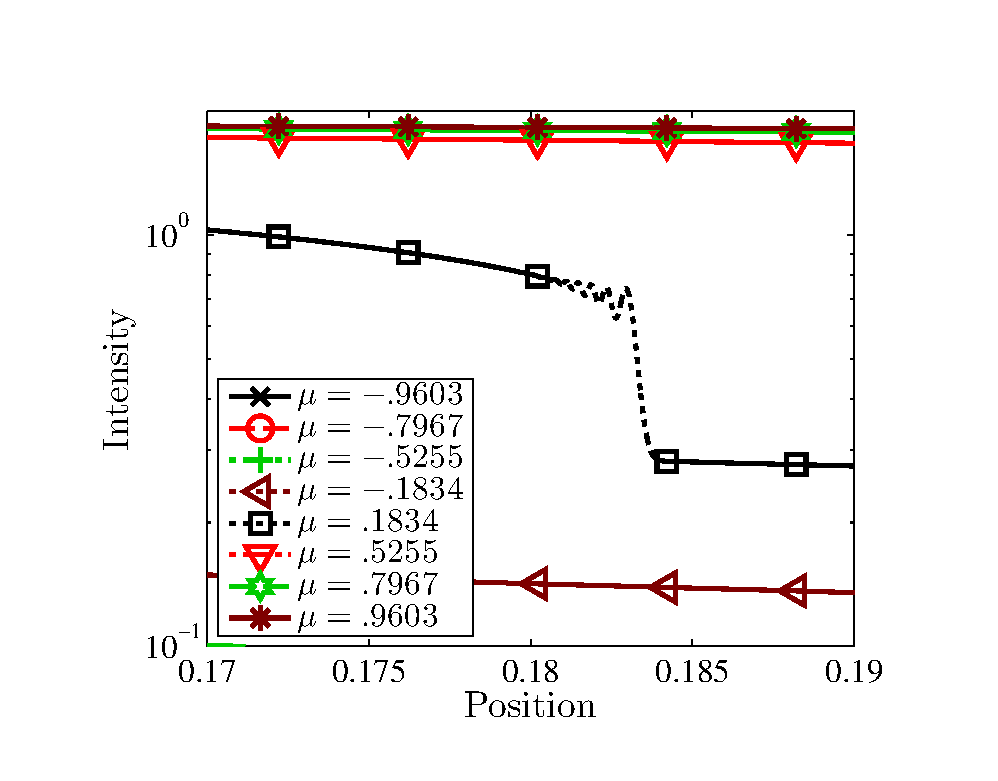
\includegraphics[height=0.8\textheight,trim=0.5in  0.2in 0.75in 0.5in,clip=true]{../chapter6_grey_radtran/Dissertation_Data/S8_pos_mu_glance_boundary_layer_log.pdf}
\end{frame}

\begin{frame}
\frametitle{$S_8$ vs $S_{32}$ Solutions}
\centering
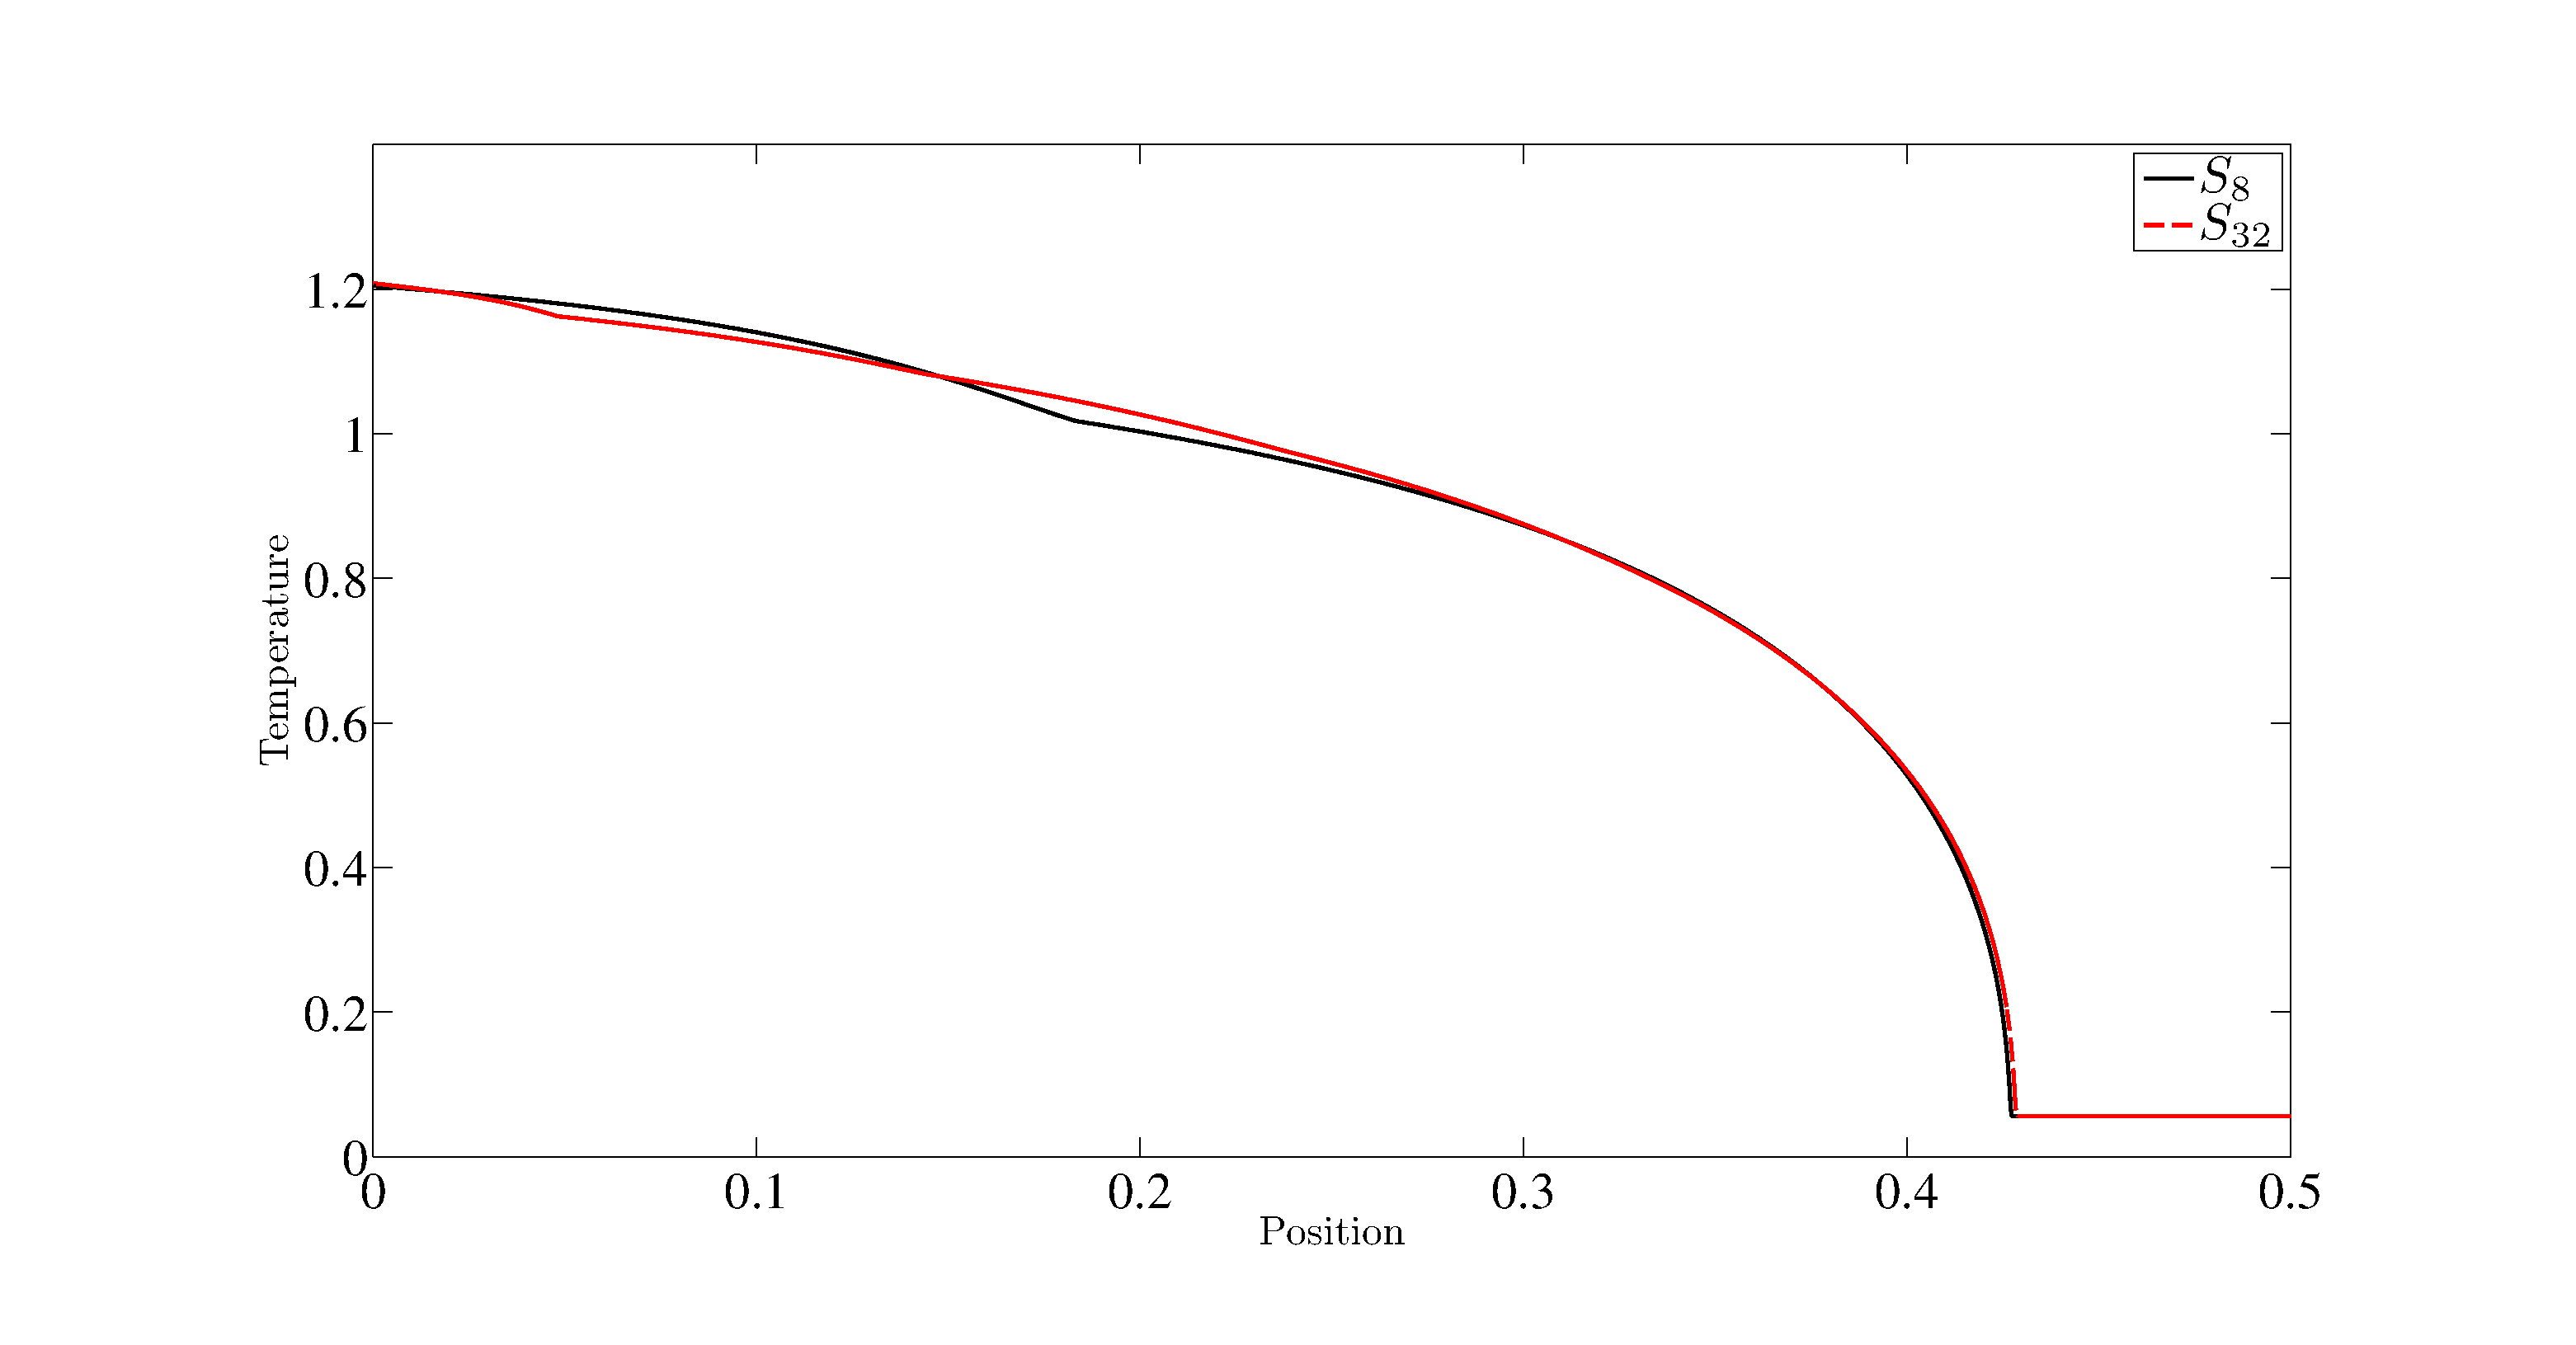
\includegraphics[width=0.75\textwidth,height=0.4\textheight,trim=1.5in  0.2in 0.5in 0.75in,clip=true]{../chapter6_grey_radtran/Dissertation_Data/S8_vs_S32_Material_Temperature.pdf}
%
\\
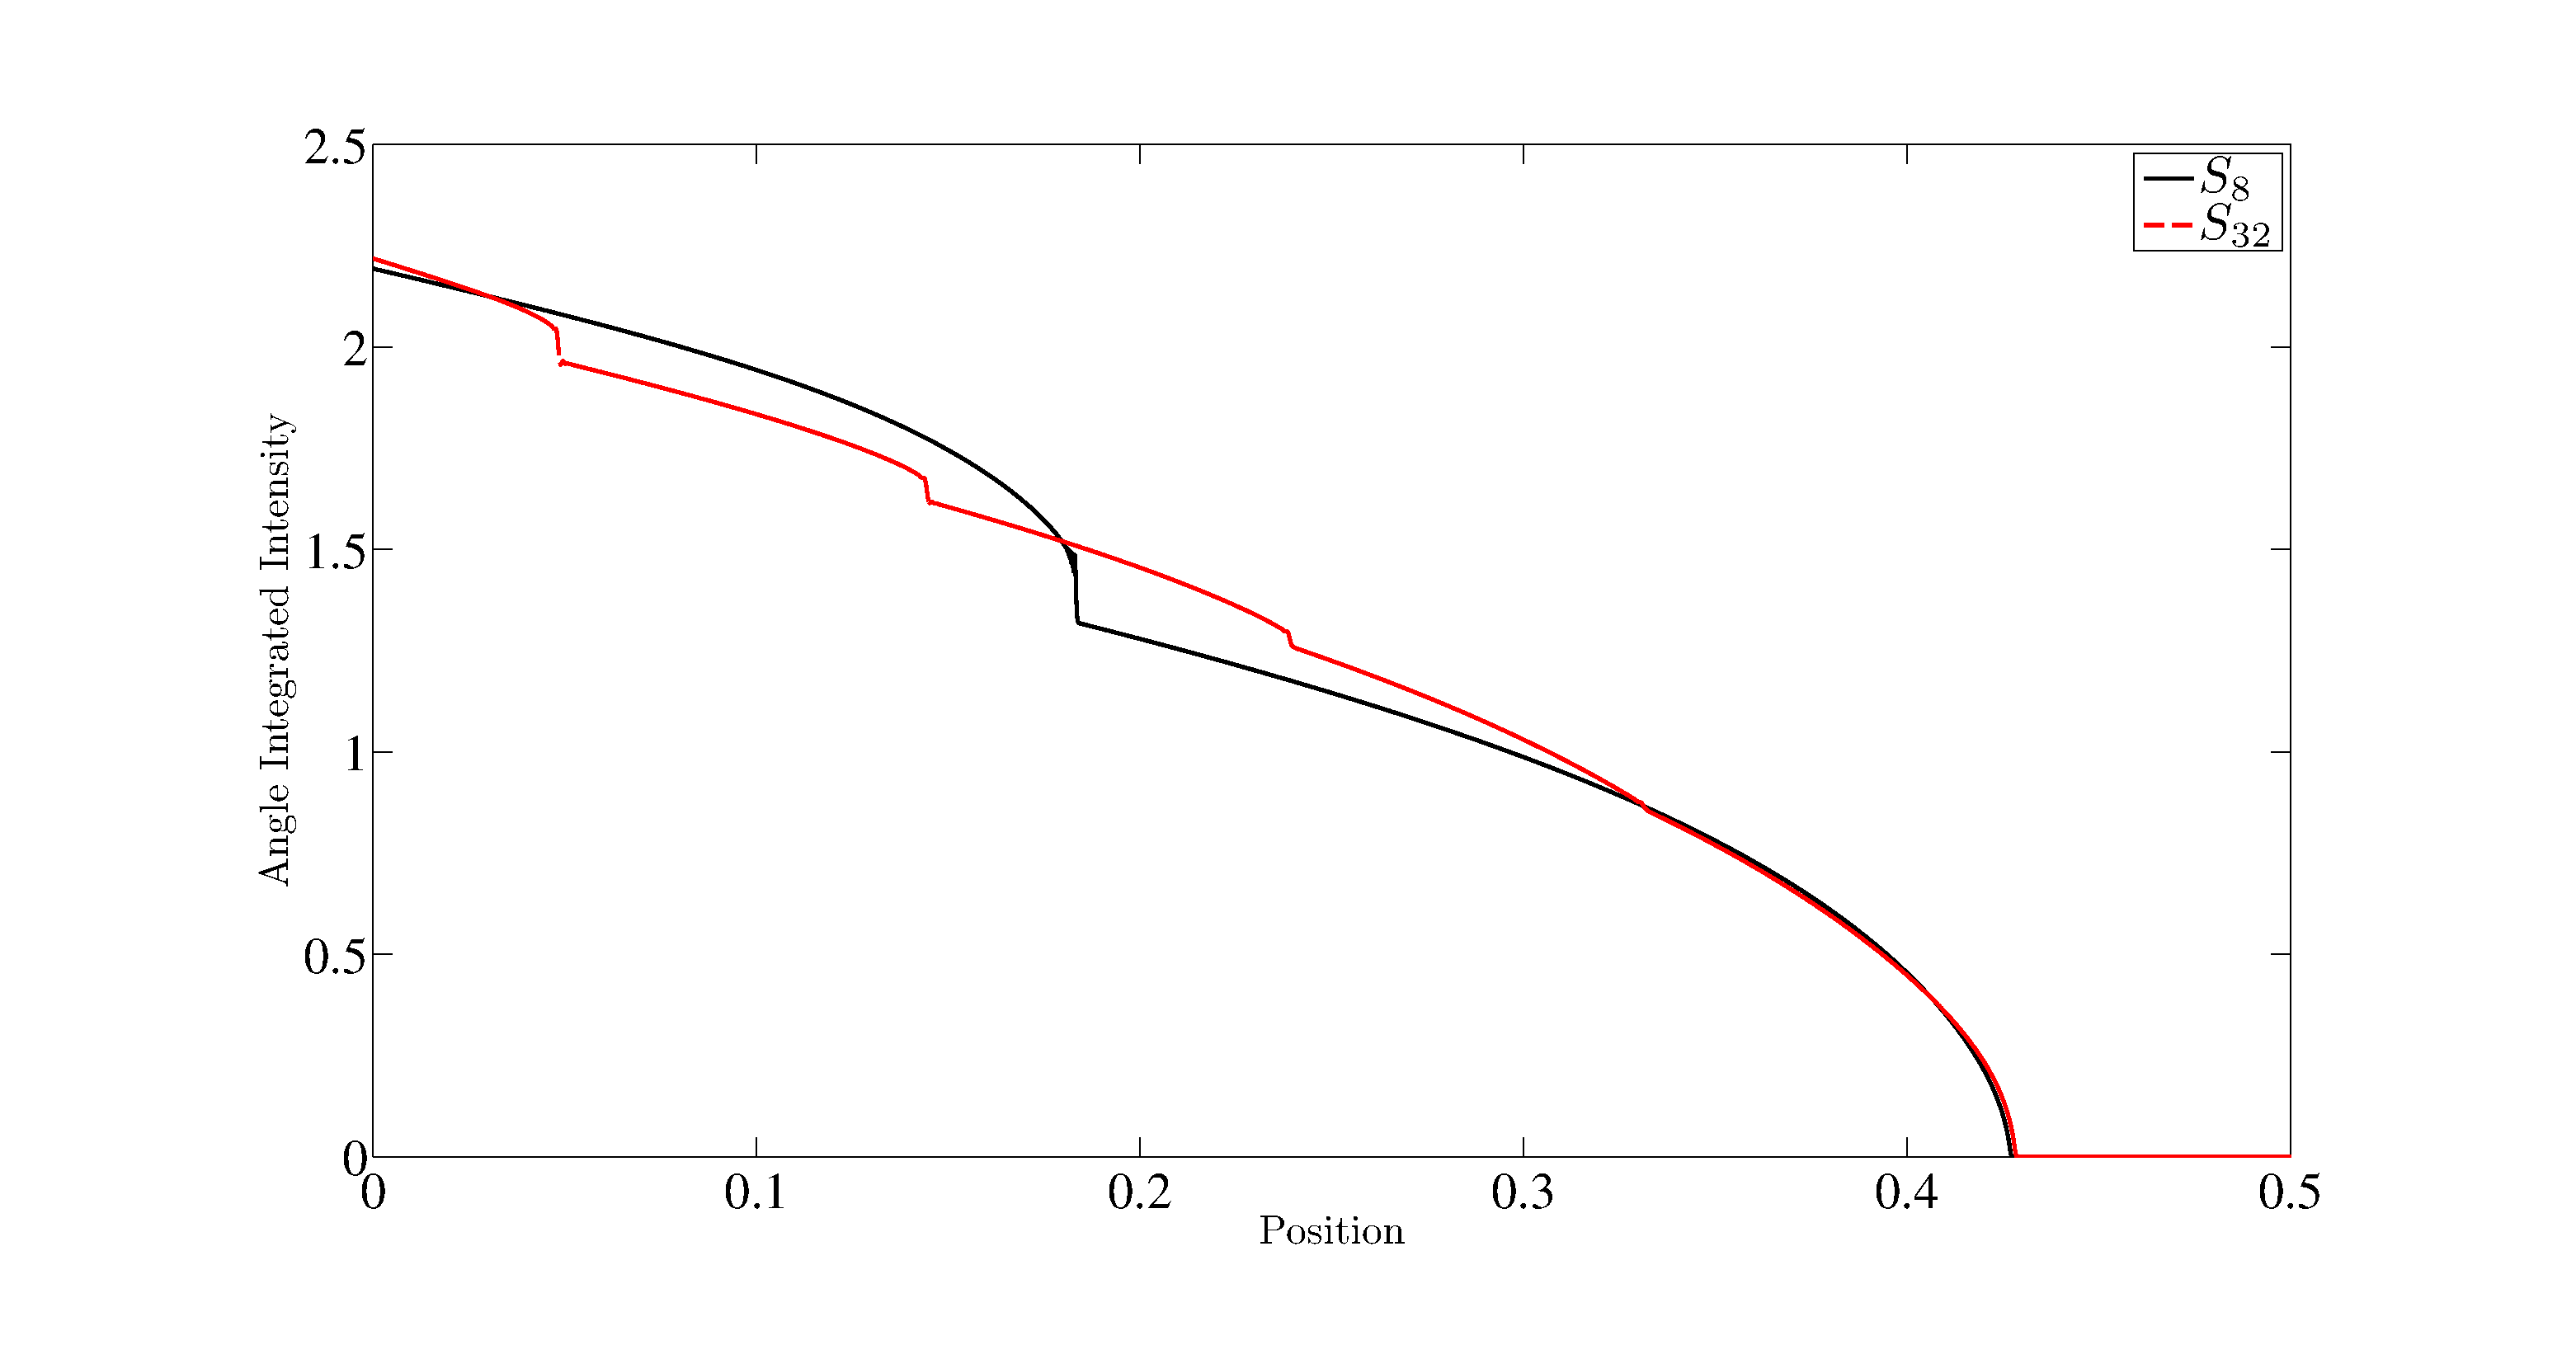
\includegraphics[width=0.75\textwidth,height=0.4\textheight,trim=1.5in  0.2in 0.5in 0.75in,clip=true]{../chapter6_grey_radtran/Dissertation_Data/S8_vs_S32_Radiation.pdf}
\\
$S_{32}$ solution- 1000 mesh cells, quartic SLXS Gauss, 5000 time steps
\end{frame}

\begin{frame}
\frametitle{$S_{32}$, $\mu_d > 0$ intensities}

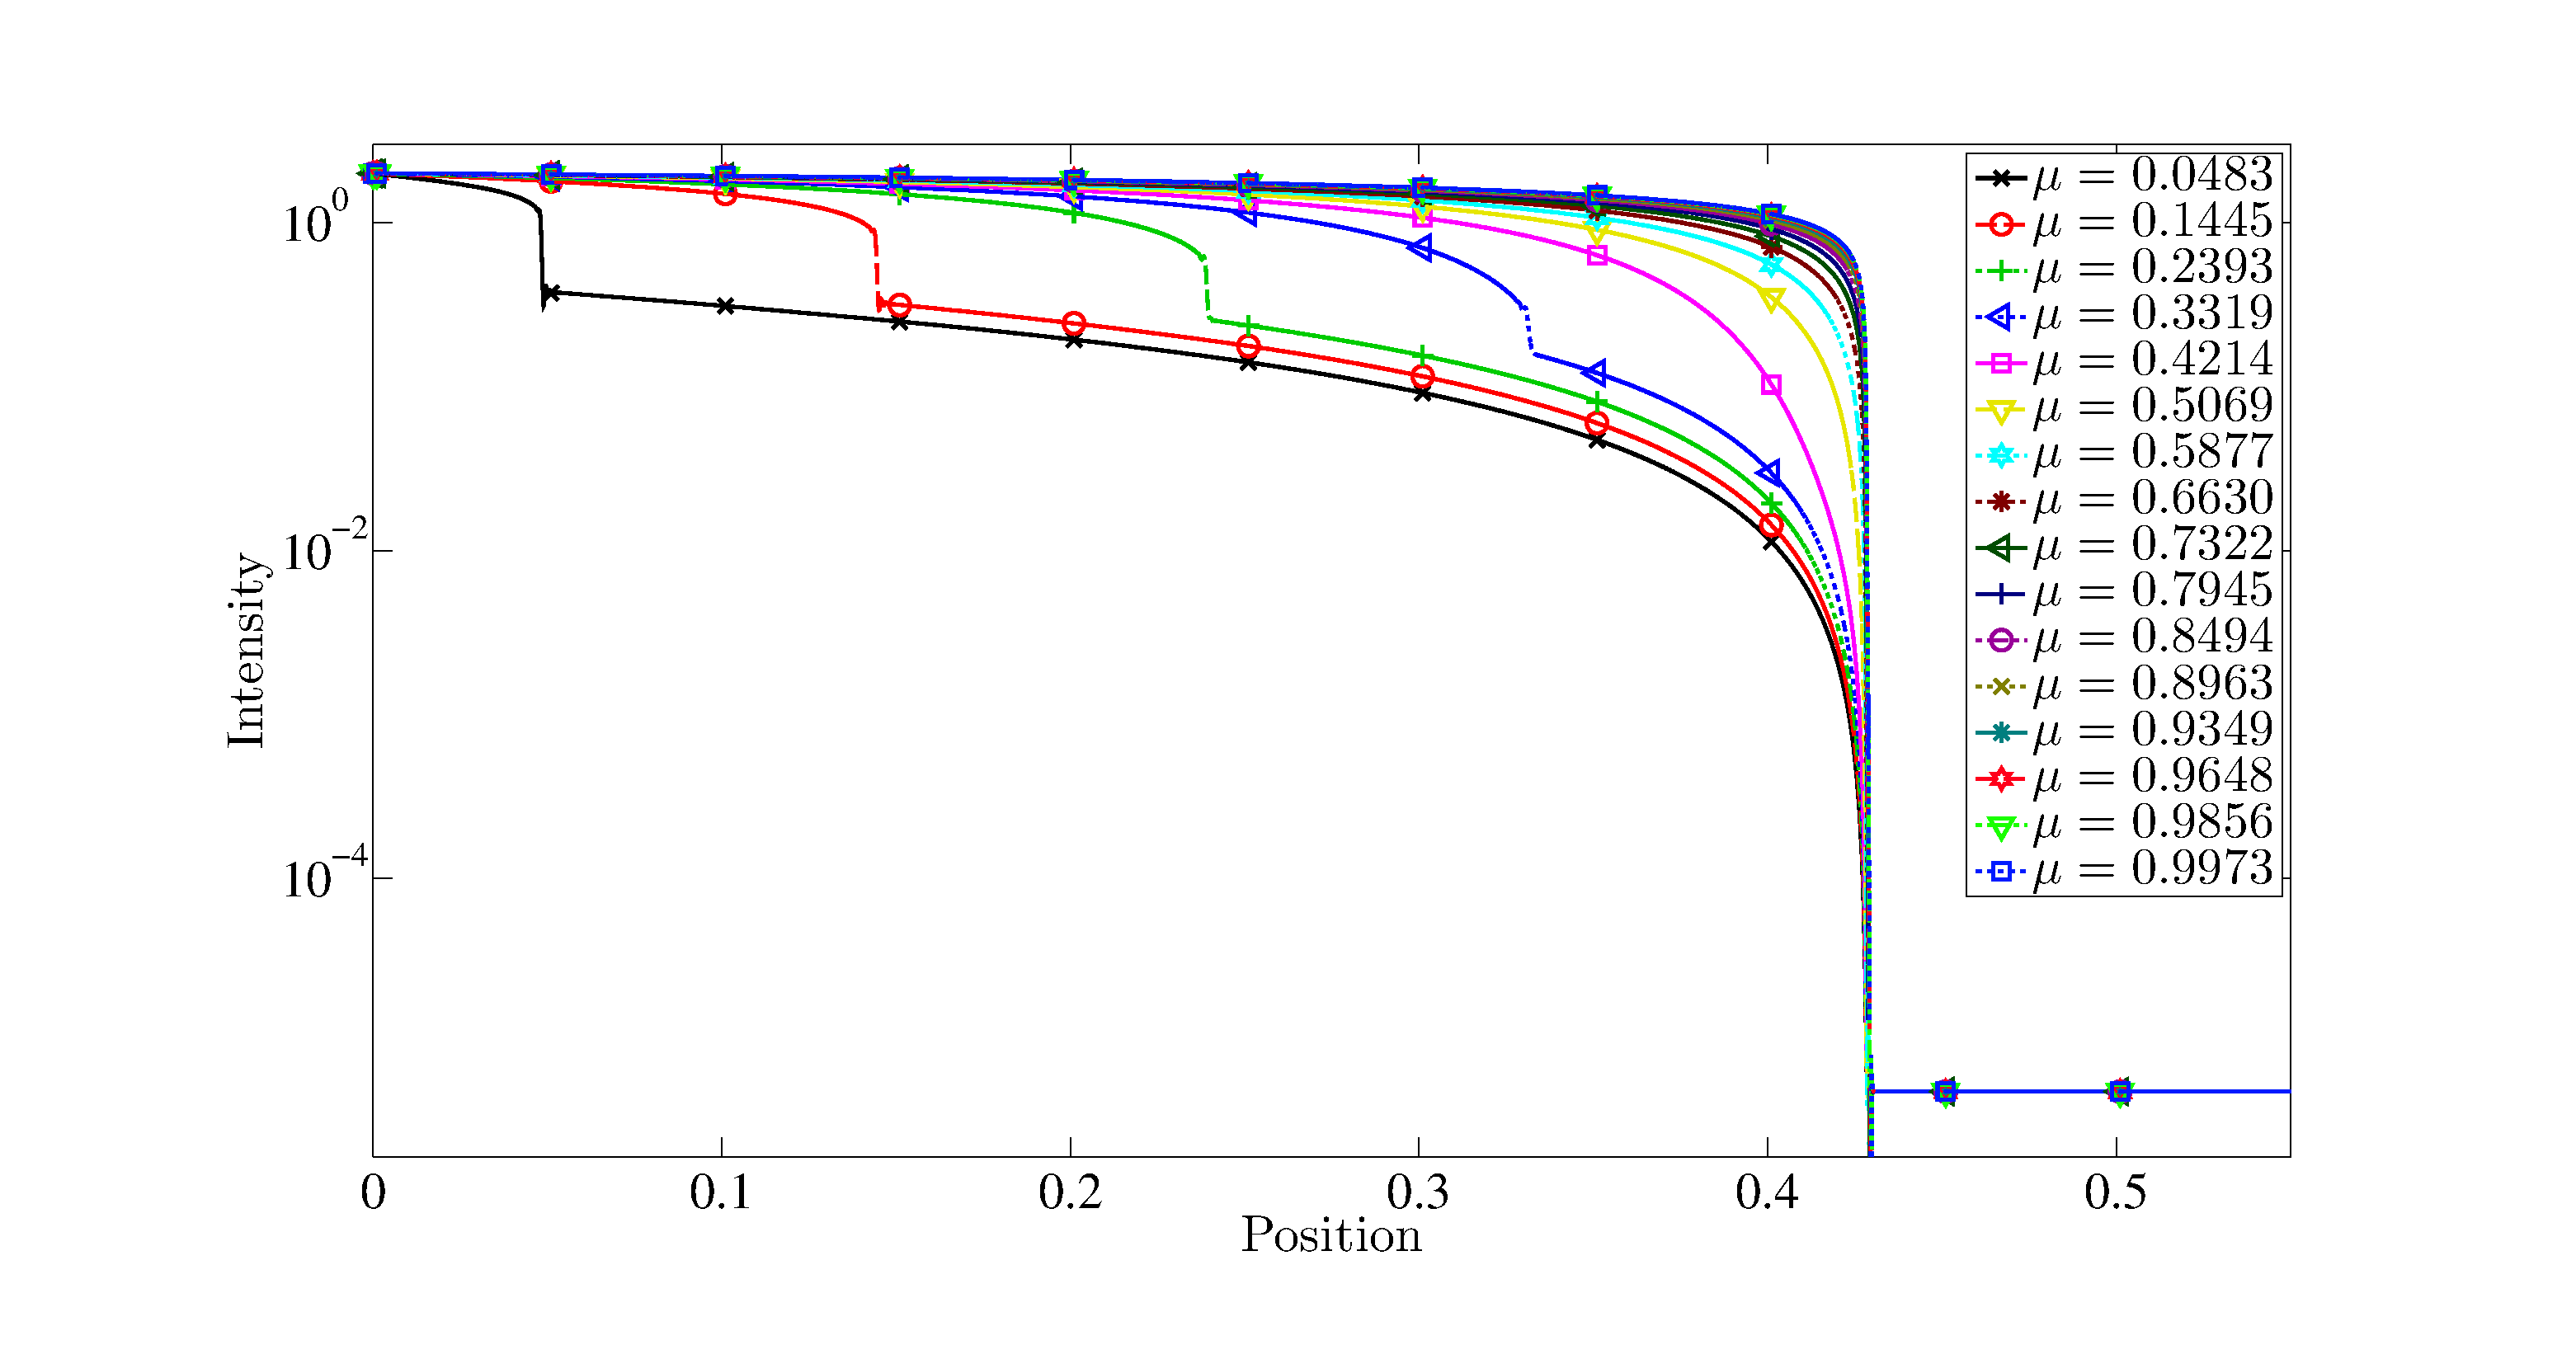
\includegraphics[width=\textwidth,trim=1.5in  0.2in 0.5in 0.75in,clip=true]{../chapter6_grey_radtran/Dissertation_Data/S32_Intensity.pdf}

\end{frame}

\section{Conclusions}
\subsection{Conclusions}
\begin{frame}
\frametitle{Conclusions}
In this research we have
\begin{enumerate}
\item Developed a matrix lumping framework that is effective for arbitrary order DFEM trial space degree
\item Demonstrated the need to consider spatial variation of material properties
\item Applied MIP diffusion operator to TRT acceleration
\item Applied higher order DFEM to grey TRT
\item Examined the asymptotic accuracy of higher order DFEM for coupled grey TRT problems
\item Generated high order, high resolution discrete ordinates results for grey TRT problems 
\end{enumerate}
\end{frame}

\subsection{Long Term Future Work}
\begin{frame}
\frametitle{Potential Future Work}
\begin{itemize}
\item Complete multi-frequency capabilities
\item Diffusion limit analysis of higher order DFEM
\item Extend lumping framework to multiple spatial dimensions
\end{itemize}
\end{frame}

\subsection{Acknowledgments}
\begin{frame}
\frametitle{Acknowledgments}
Thanks for your time!
\vspace{0.3in}
Portions of this work were funded by the Department of Energy CSGF program, administered by the Krell Institute, under grant DE-FG02-97ER25308.
\\
\vspace{0.3in}
Additional support was provided by the Department of Energy, National Nuclear Security Administration, under Award Number(s) DE-NA0002376.

\end{frame}

% %%%%%%%%%%%%%%%%%%%%%%%%%%%%%%%%%%%%%%%%%%%%%%%%%%%%%%%%%%%%%%%%%%%%%%%%%%%%%%%%%
\appendix
% %%%%%%%%%%%%%%%%%%%%%%%%%%%%%%%%%%%%%%%%%%%%%%%%%%%%%%%%%%%%%%%%%%%%%%%%%%%%%%%%%
\subsection{Spatially Constant Cross Section}

\begin{frame}
\frametitle{Test Problem}
Source-free pure absorber, left incident flux, $\psi_{in,d}$, vacuum right BC.

Defining $h$:
\be
h = \frac{\sigma_t \Delta x}{\mu_d}
\ee
Analytic solution is
\be
\psi(x,\mu_d) = \psi_{in,d} \exp[-h]
\ee

\end{frame}

\begin{frame}
\frametitle{Order of Convergence}
Convergence of $\norm{ \widetilde{\psi} - \psi }_{L^2}$ as a function of $h$ 
\begin{columns}[c]
\column{0.5\textwidth}
\begin{figure}
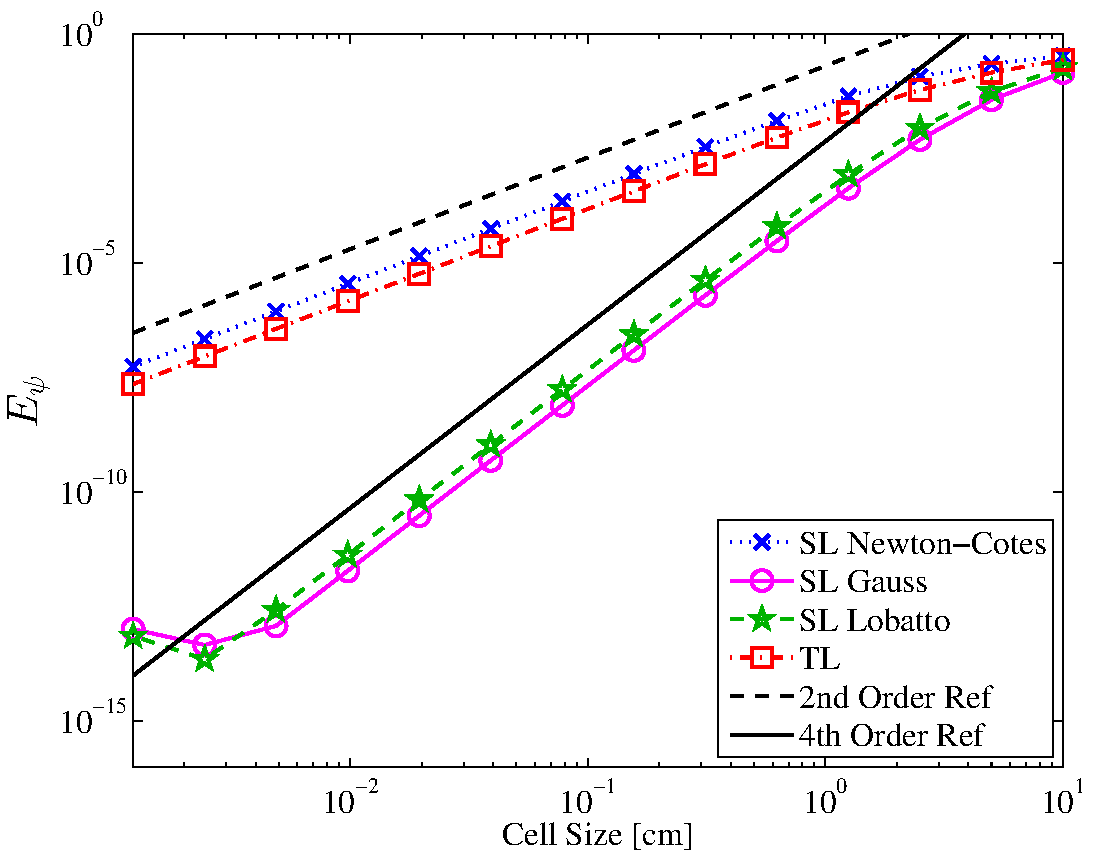
\includegraphics[width=5.5cm]{../chapter2_constant_xs/Cubic_L2_err-eps-converted-to.pdf}
\caption{$P=3$.}
\end{figure}
\column{0.5\textwidth}
\begin{figure}
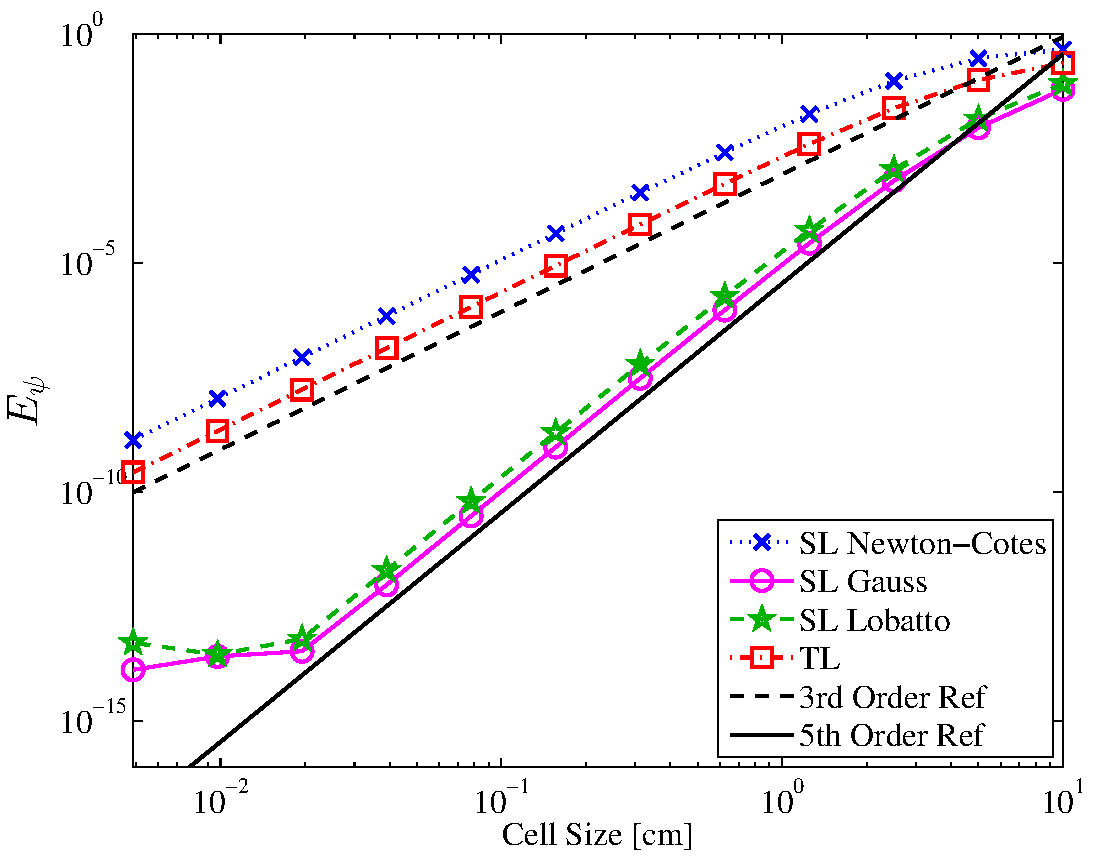
\includegraphics[width=5.5cm]{../chapter2_constant_xs/Quartic_L2_err-eps-converted-to.pdf}
\caption{$P=4$}
\end{figure}
\end{columns}
\end{frame}


\begin{frame}
\frametitle{Summary of Constant Cross Section Discoveries}
Positivity
\begin{itemize}
\item SL Gauss is strictly positive for even $P$
\item SL Lobatto and SL Newton-Cotes: strictly positive for odd $P$
\item TL not robust for $P>1$
\end{itemize}
Accuracy
\begin{itemize}
\item TL and SL Newton-Cotes converge $\norm{ \widetilde{\psi} - \psi }_{L^2} $ 2nd order for odd $P$, 3rd order for even $P$
\item SL Lobatto and SL Gauss converge $\norm{ \widetilde{\psi} - \psi }_{L^2} \propto P+1$
\end{itemize}
Equivalence
\begin{itemize}
\item SL Gauss equivalent to Exact DFEM for all $P$
\item TL = SL Lobatto = SL Newton-Cotes for $P=1,2$
\end{itemize}
\end{frame}

\subsection{Spatially Varying Cross Section}

\begin{frame}
\frametitle{Test Problem}
\begin{itemize}
\item Spatially varying cross section of the form:
\be
\sigma_t(x) = c_1 e^{c_2 x}
\ee
\item Incident flux, $\psi_{in,d}$ on the left, vacuum on the right, no sources.
\item Analytic Solution
\be
\psi(\mu_d,x) = \psi_{in,d}\exp\left[ \frac{c_1 }{\mu_d c_2 } \left(1- e^{c_2 x}  \right) \right] 
\ee
\end{itemize}
\end{frame}

\begin{frame}
\frametitle{Additional Numerical Schemes}
\begin{itemize}
\item {\bf CXS DFEM}: Equally-spaced interpolation points, analytic integration.  Approximate cross section by cell average value
\item {\bf SLXS Lobatto}: Lobatto interpolation points, self-lumping extended to account for cross section variation
\item {\bf SLXS Gauss}: Gauss interpolation points, self-lumping extended to account for cross section variation
\item {\bf SLXS Newton-Cotes}: Equally-spaced interpolation points, self-lumping extended to account for cross section variation
\end{itemize}
We will no longer consider the TL scheme.
\end{frame}

\begin{frame}
\frametitle{Convergence Results}
We examine the convergence of $E_{\psi}$ and $E_{\psi_{out}}$ for a pure absorber with
\be
\sigma_t(x) = 0.1~10^{2x}
\ee
and $x\in[0,1~cm]$.  We define the error quantities as:
\bea
E_{\psi} &=& \norm{ \widetilde{\psi}_d(x) - \psi(x,\mu_d)  }_{L^2} \\
E_{\psi_{out}} &=& \sqrt{\sum_{i=1}^{N_{cells}}{\Delta x_i\left(\widetilde{\psi}_{out,i} - \psi(x_{i+1/2})  \right)^2   }}  
\eea
\end{frame}

\begin{frame}
\frametitle{$L^2$ Convergence}
New Result: SLXS Lobatto and SLXS Gauss are accurate methods for spatially varying cross section problems
\begin{columns}[c]
\column{0.45\textwidth}
\begin{figure}
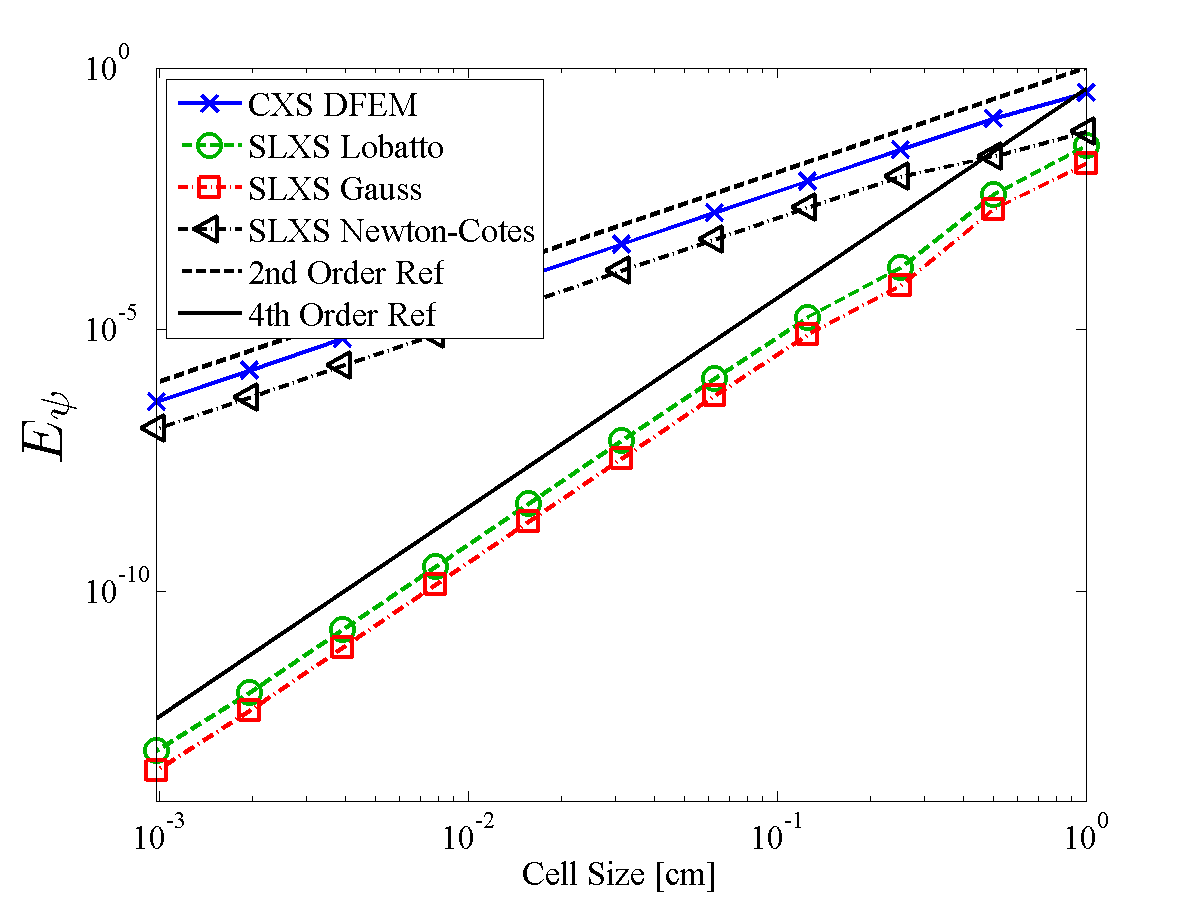
\includegraphics[width=5cm]{../chapter3_variable_xs/P3_VarXS_E_psi_L2.png}
\caption{$P=3$ convergence plot.}
\end{figure}
\column{0.55\textwidth}
Summary of Convergence Orders
\begin{itemize}
\item SLXS Gauss: $\propto P+1$
\item SLXS Lobatto: $\propto P+1$, less accurate than SL Gauss
\item SLXS Newton-Cotes: 2 if odd $P$, 3 if even $P$
\item CXS DFEM: 2 regardless of $P$
\end{itemize}
\end{columns}
\end{frame}

\subsection{Interaction Rate}

\begin{frame}
\frametitle{Interaction Rate}
\begin{itemize}
\item Analytic interaction rate
\be
 IR(x) = \sigma_t(x) \psi(x,\mu_d)
\ee
\item CXS DFEM approximation
\be
\widetilde{IR}(x) = \hat{\sigma}_t \widetilde{\psi}(x)
\ee
\item SLXS schemes:  Only point-wise knowledge of $\sigma_t(x)$ in DFEM equations
\begin{itemize}
\item Integrals: evaluate $\widetilde{IR}(x)$ with quadrature restricted to interpolation points
\item Plotting purposes:
\be
\widetilde{IR}(x) = \sum_{j=1}^{P+1}{ \sigma_{t,j} \psi_j \B{j}(s) } 
\ee
\end{itemize}
\end{itemize}
\end{frame}

\begin{frame}
\frametitle{$L^2$ error of $\widetilde{IR}(x)$}

New Result: SLXS Lobatto and SLXS Gauss Accurately Approximate $\widetilde{IR}(x)$
\begin{columns}[c]
\column{0.55\textwidth}
\begin{figure}
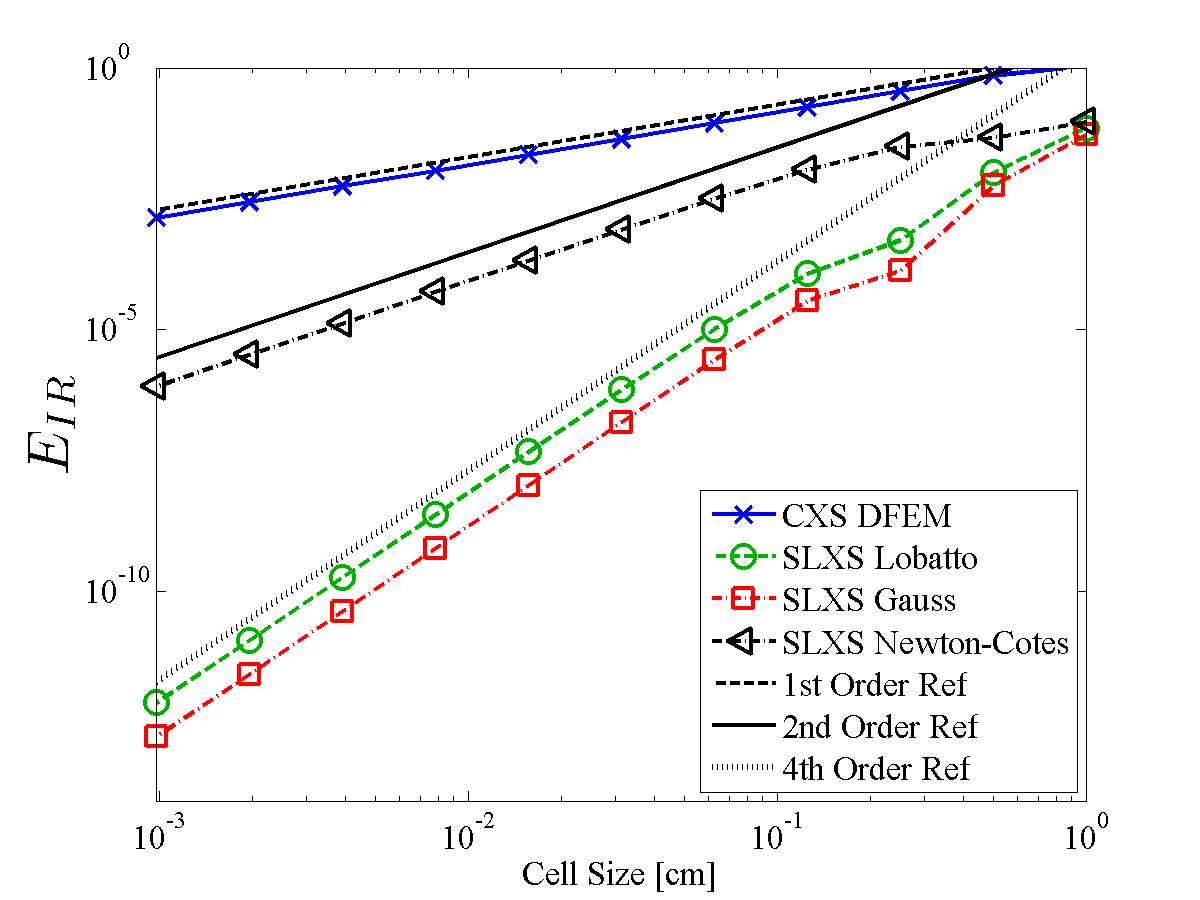
\includegraphics[width = 5cm]{../chapter3_variable_xs/P3_VarXS_E_I_L2.png}
\caption{Cubic DFEM}
\end{figure}
\column{0.45\textwidth}
Summary of Convergence Orders
\begin{itemize}
\item SL Gauss: $P+1$
\item SL Lobatto: $P+1$
\item SL Newton-Cotes: 2 for odd $P$, 3 for even $P$
\item CXS DFEM: 1, regardless of trial space degree
\end{itemize}
\end{columns}
\end{frame}


\begin{frame}
\frametitle{$E_{IR_A}$ Convergence}
\begin{columns}[c]
\column{0.45\textwidth}
\begin{figure}
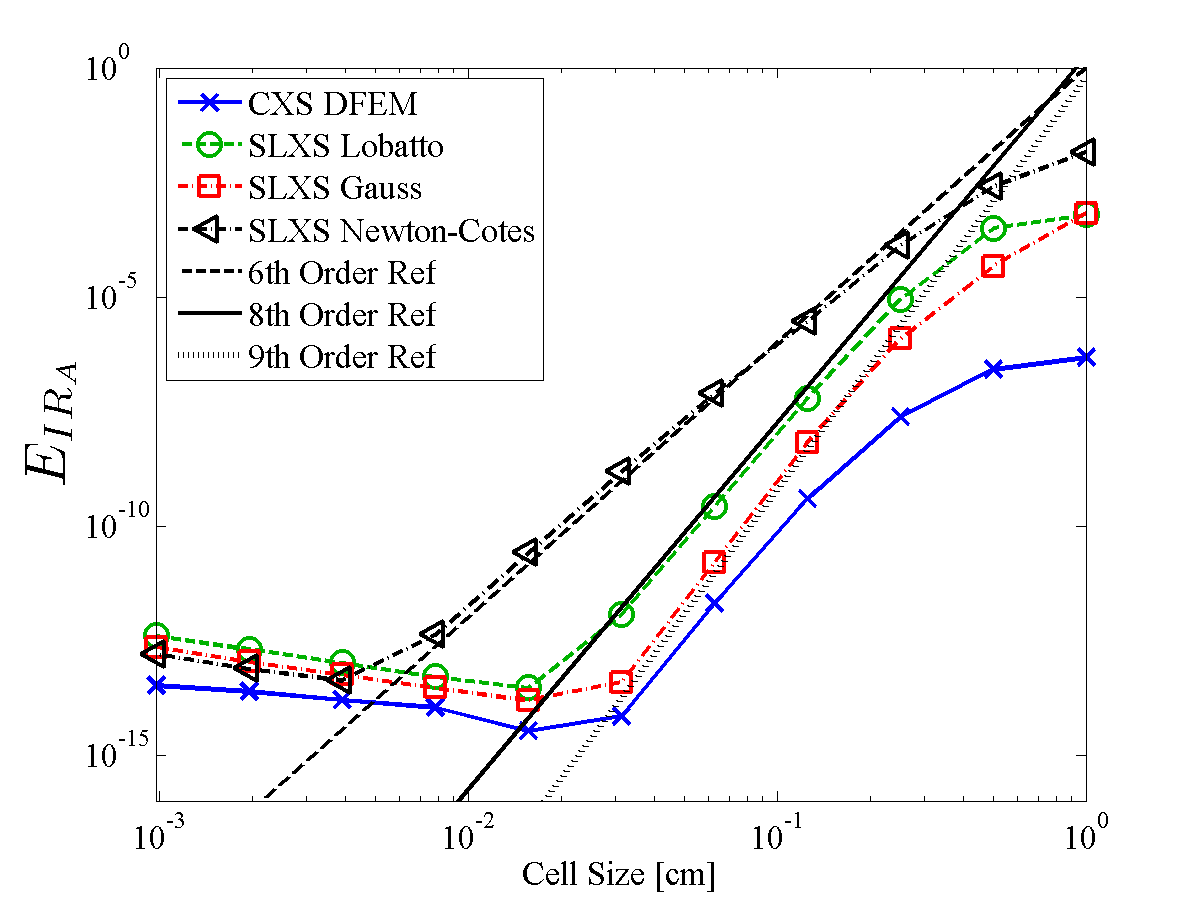
\includegraphics[width = 5cm]{../chapter3_variable_xs/P4_VarXS_E_I_A.png}
\caption{Quartic DFEM}
\end{figure}
\column{0.55\textwidth}
Summary of Convergence Orders
\begin{itemize}
\item SL Gauss: $2P+1$
\item SL Lobatto: $2P$
\item SL Newton-Cotes: $P+1$ for odd $P$, $P+2$ for even $P$
\item CXS DFEM: $2P+1$, regardless of trial space degree
\end{itemize}
\end{columns}
\end{frame}

\begin{frame}
\frametitle{CXS DFEM Accuracy Calculating $IR_A$}
\begin{itemize}
\item How can CXS DFEM converge $E_{IR_A}$ so accurately?
\item Local Conservation
\be
\text{Particles In} - \text{Particles Out} =  \text{Total Interactions} 
\ee
\item Particles In: Outflow from Previous Cell
\item Particles Out: Outflow from Current Cell
\item CXS DFEM converges angular flux outflow $\propto 2P+1$
\item $\therefore$ CXS DFEM accurately calculates
\be
\text{Total Interactions} =\Delta x \left( \widetilde{IR}_A \right)
\ee
\end{itemize}
\end{frame}


\subsection{Blading}
\begin{frame}
\frametitle{CXS DFEM Interaction Rate Profile}

\begin{block}{New to Dissertation}
Observation and explanation of blading phenomena
\end{block}
\begin{columns}[c]
\column{0.5\textwidth}
\begin{figure}
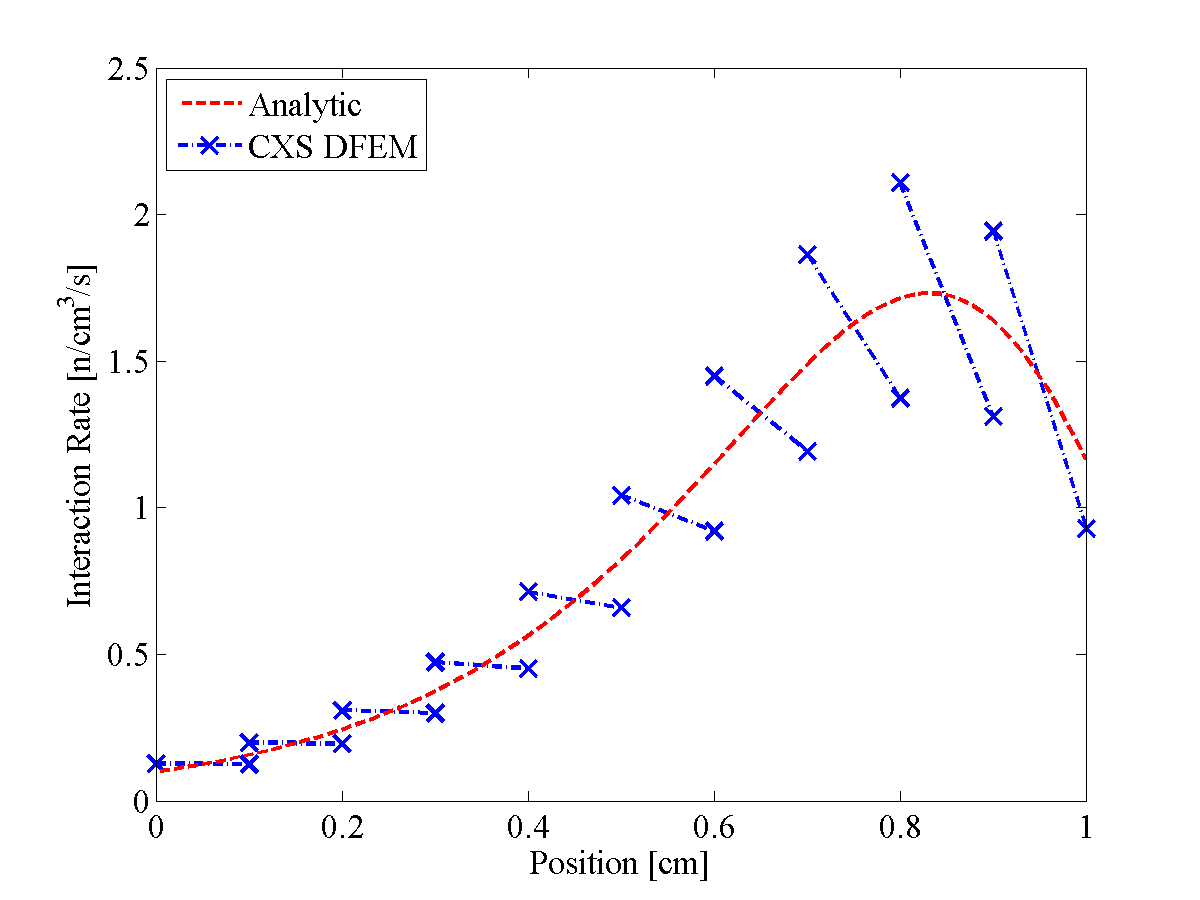
\includegraphics[width=5cm]{../chapter3_variable_xs/CXS_I_Profile.png}
\caption{$\widetilde{IR}(x)$ profile.}
\end{figure}
\column{0.5\textwidth}
\begin{figure}
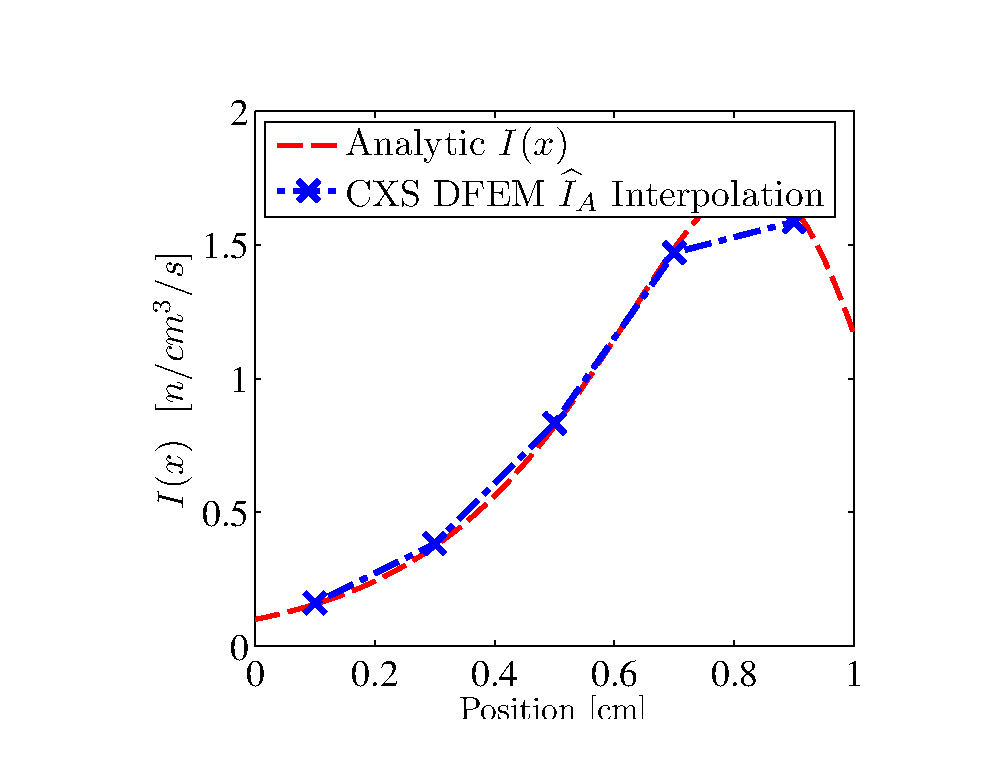
\includegraphics[width=5cm]{../chapter3_variable_xs/CXS_I_A_Profile.pdf}
\caption{Interpolated $\widetilde{IR}_A$ profile.}
\end{figure}
\end{columns}

\end{frame}


\begin{frame}
\frametitle{Something Wrong with DFEM?}
No.  Consider the analytic solution to a problem that has the cell-wise average cross section.
\begin{columns}[c]
\column{0.5\textwidth}
\begin{figure}
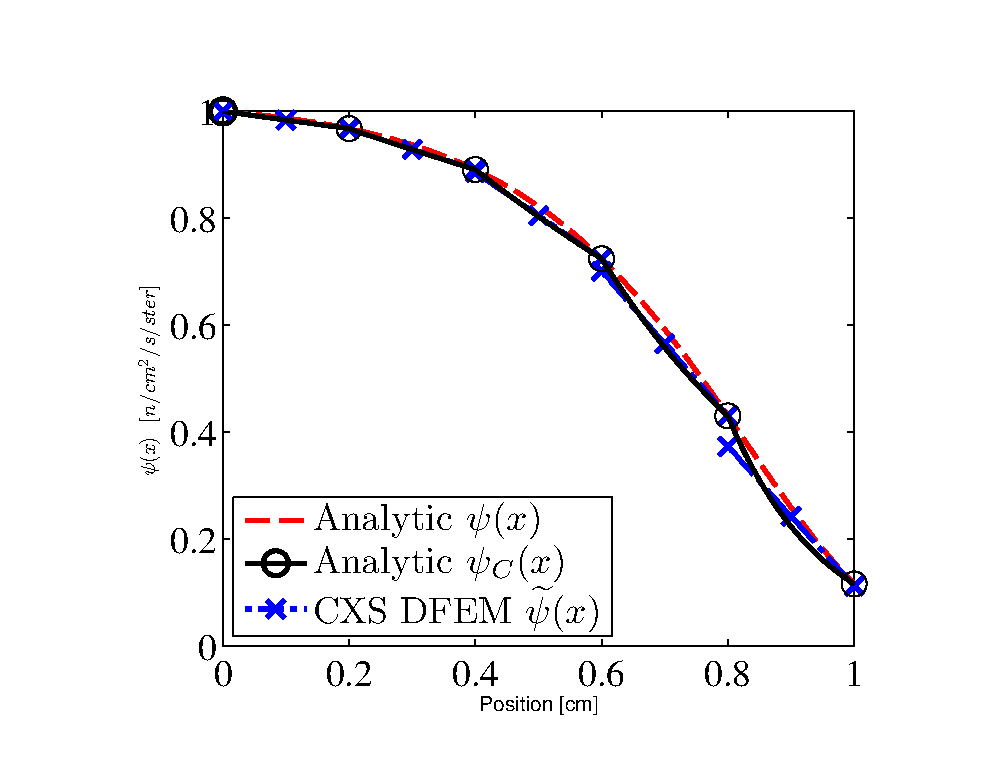
\includegraphics[width=5cm]{../chapter3_variable_xs/Psi_Blades.pdf}
\caption{Angular Flux.}
\end{figure}
\column{0.5\textwidth}
\begin{figure}
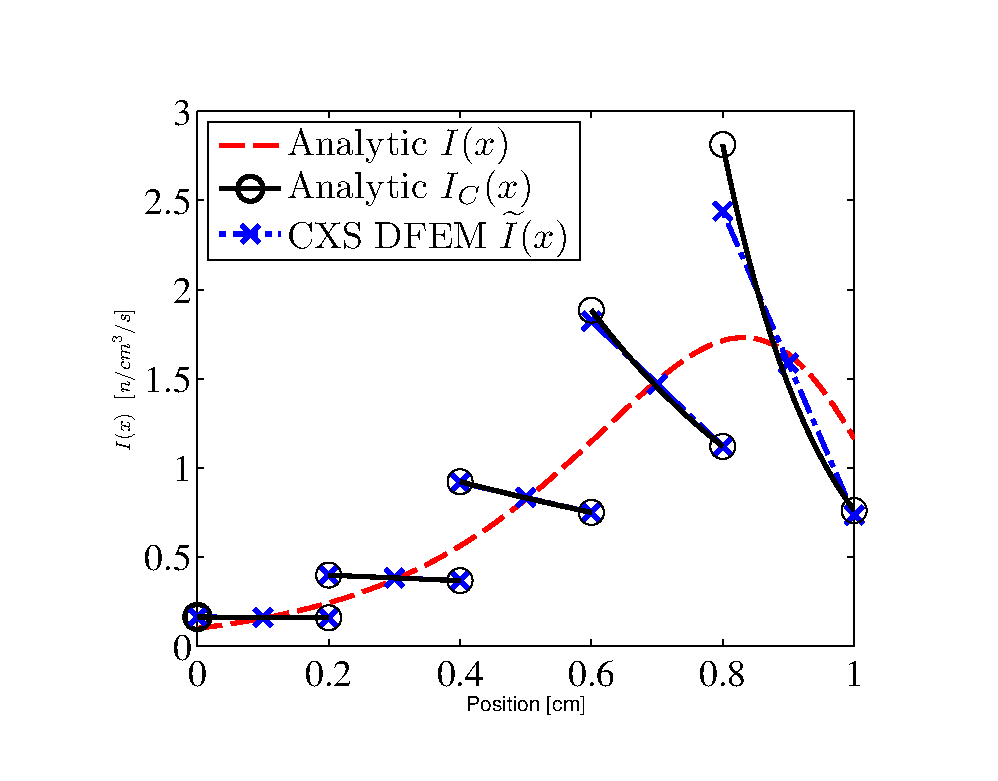
\includegraphics[width=5cm]{../chapter3_variable_xs/I_Blades.pdf}
\caption{Interaction Rate.}
\end{figure}
\end{columns}

\end{frame}

\begin{frame}
\frametitle{Linear SL Lobatto Solution}
\begin{block}{New to Dissertation}
New: Self-lumping schemes do not exhibit blading
\end{block}
\begin{columns}[c]
\column{0.5\textwidth}
\begin{figure}
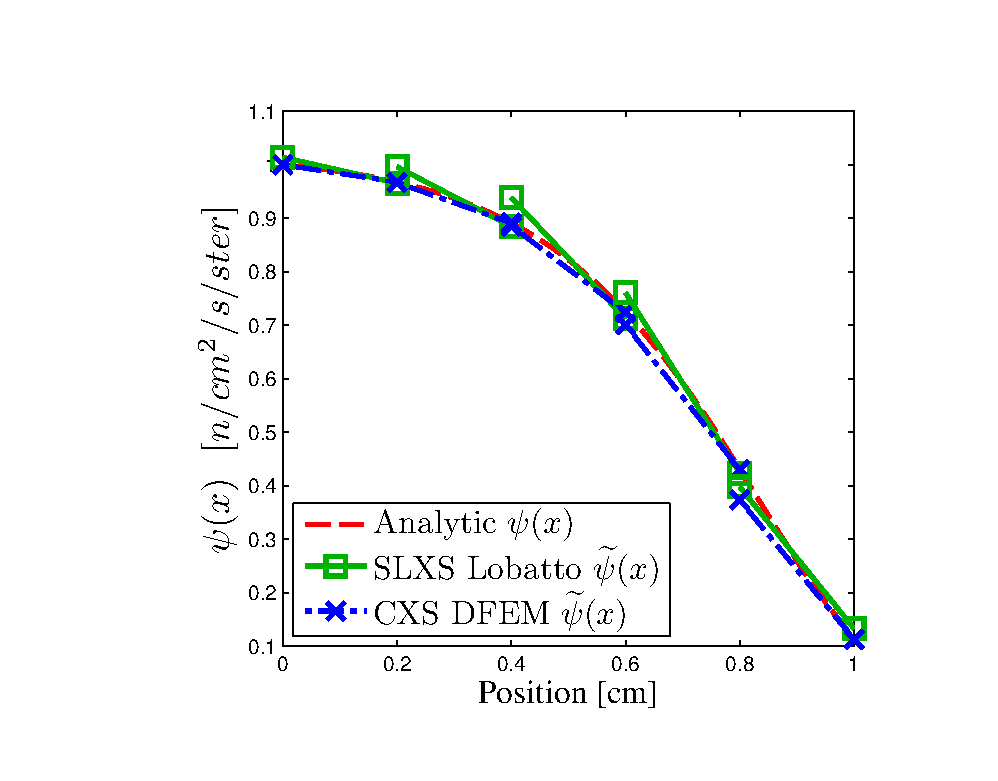
\includegraphics[width=5cm]{../chapter3_variable_xs/SLXS_Psi_Profile.pdf}
\caption{Angular Flux.}
\end{figure}
\column{0.5\textwidth}
\begin{figure}
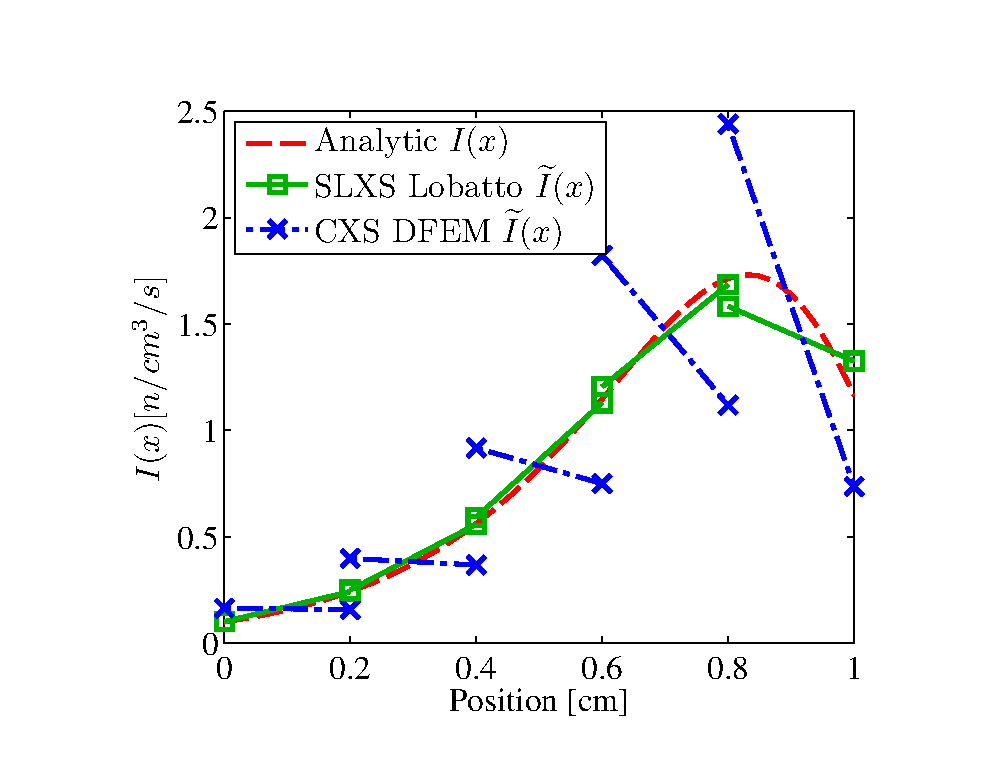
\includegraphics[width=5cm]{../chapter3_variable_xs/SLXS_I_Profile.pdf}
\caption{Interaction Rate.}
\end{figure}
\end{columns}
\end{frame}
%%%%%%%%%%%%%%%%%%%%%%%%%%%%%%%%%%%%%%%%%%%%%%%%%%%%%%%%%%%%%%%%%%%%%%%%%%%%%%%%%

\subsection{TRT Results}

\begin{frame}
\frametitle{Constant Material Properties- MMS1}
\bea
M(\mu_d) &=& \frac{1}{4\pi} \\
F(t) &=& 1+.02t \\
W_I(x) &=& 10 \cos\left( \frac{\pi x}{10} - \frac{\pi}{2} \right) + 15 \\
W_T(x) &=& 25 \cos\left( \frac{\pi x}{10} - \frac{\pi}{2} \right) + 30 \\
C_v &=& 0.1 \\
\sigma_a &=& 100 \\ 
\sigma_s &=& 0.5 \\
t &\in& [0,1] \\
\Delta t &=& 0.01 \\
\eea
Used $S_8$ quadrature, 2-2 SDIRK scheme
\end{frame}

\begin{frame}
\frametitle{TL- MMS1 Results}
TL does not get better applied to a harder problem
\begin{columns}[t]
\column{0.5\textwidth}
\centering
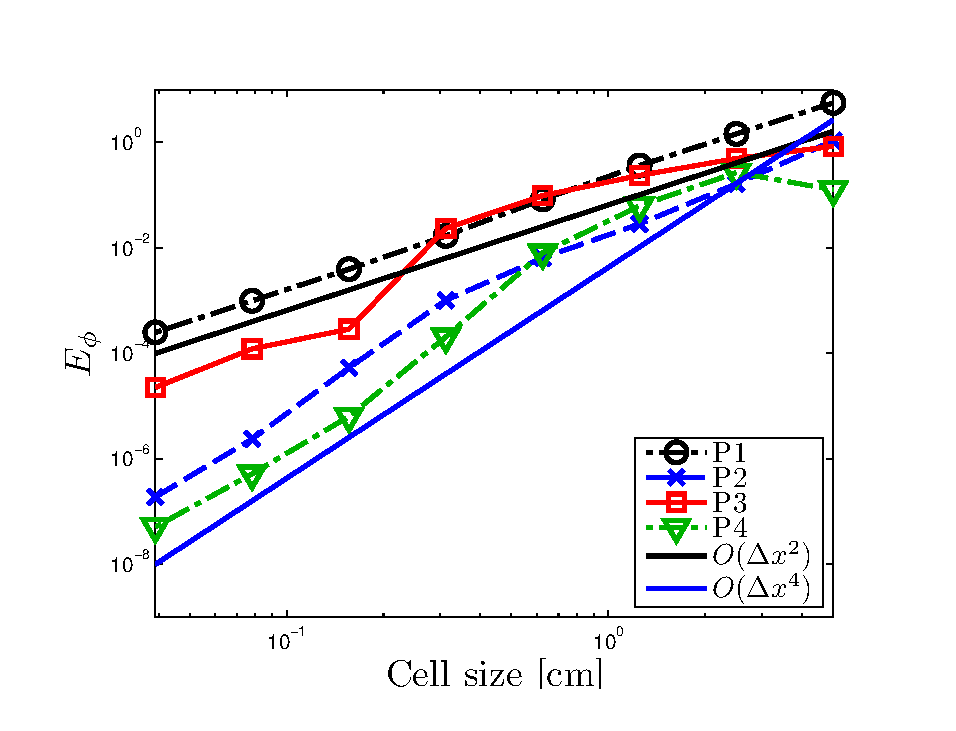
\includegraphics[width=\textwidth,trim=0.25in  0.2in 0.75in 0.5in,clip=true]{../chapter6_grey_radtran/Dissertation_Data/MMS2_TL_phi_L2.pdf}
\column{0.5\textwidth}
\centering
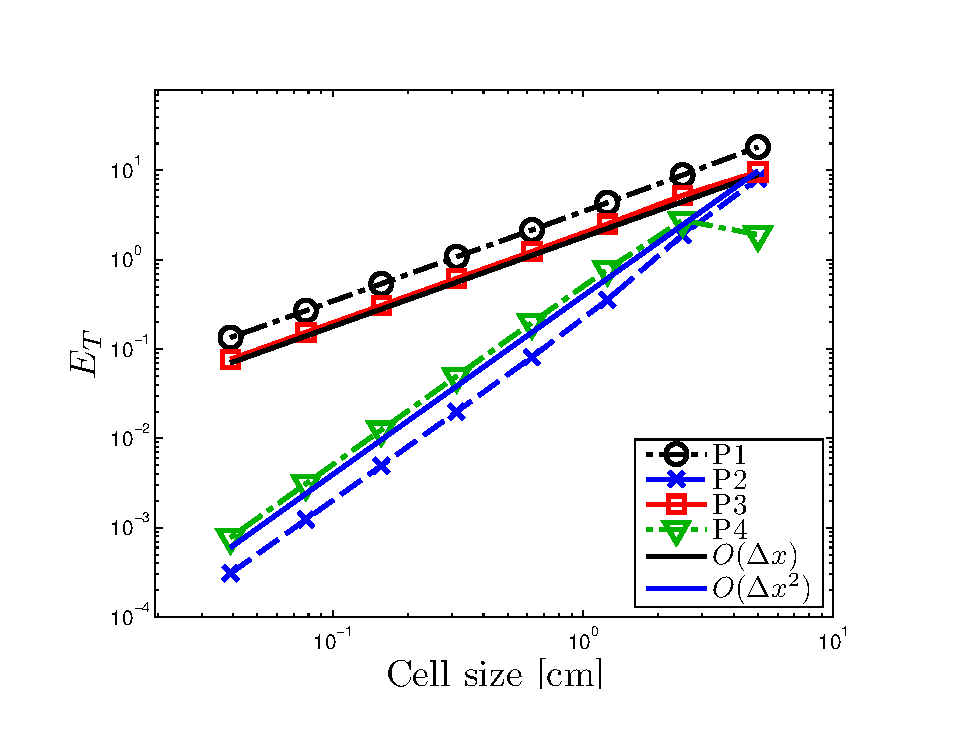
\includegraphics[width=\textwidth,trim=0.25in  0.2in 0.75in 0.5in,clip=true]{../chapter6_grey_radtran/Dissertation_Data/MMS2_TL_temp_L2.pdf}
\end{columns}
\end{frame}

\begin{frame}
\frametitle{SL Lobatto- MMS1 Results}
SL Lobatto loses an order in $T$
\begin{columns}[t]
\column{0.5\textwidth}
\centering
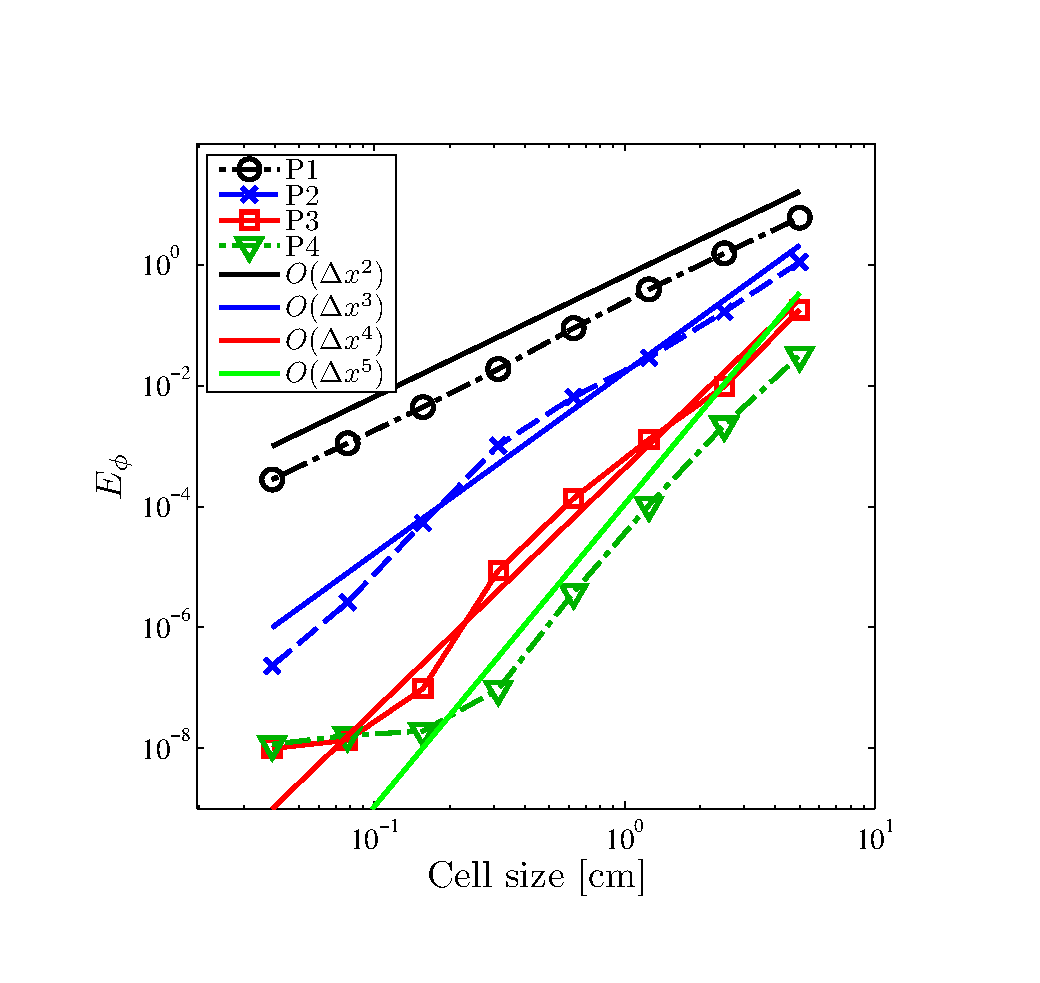
\includegraphics[width=\textwidth,trim=0.25in  0.2in 0.75in 0.5in,clip=true]{../chapter6_grey_radtran/Dissertation_Data/MMS2_SLXS_Lobatto_phi_L2.pdf}
\column{0.5\textwidth}
\centering
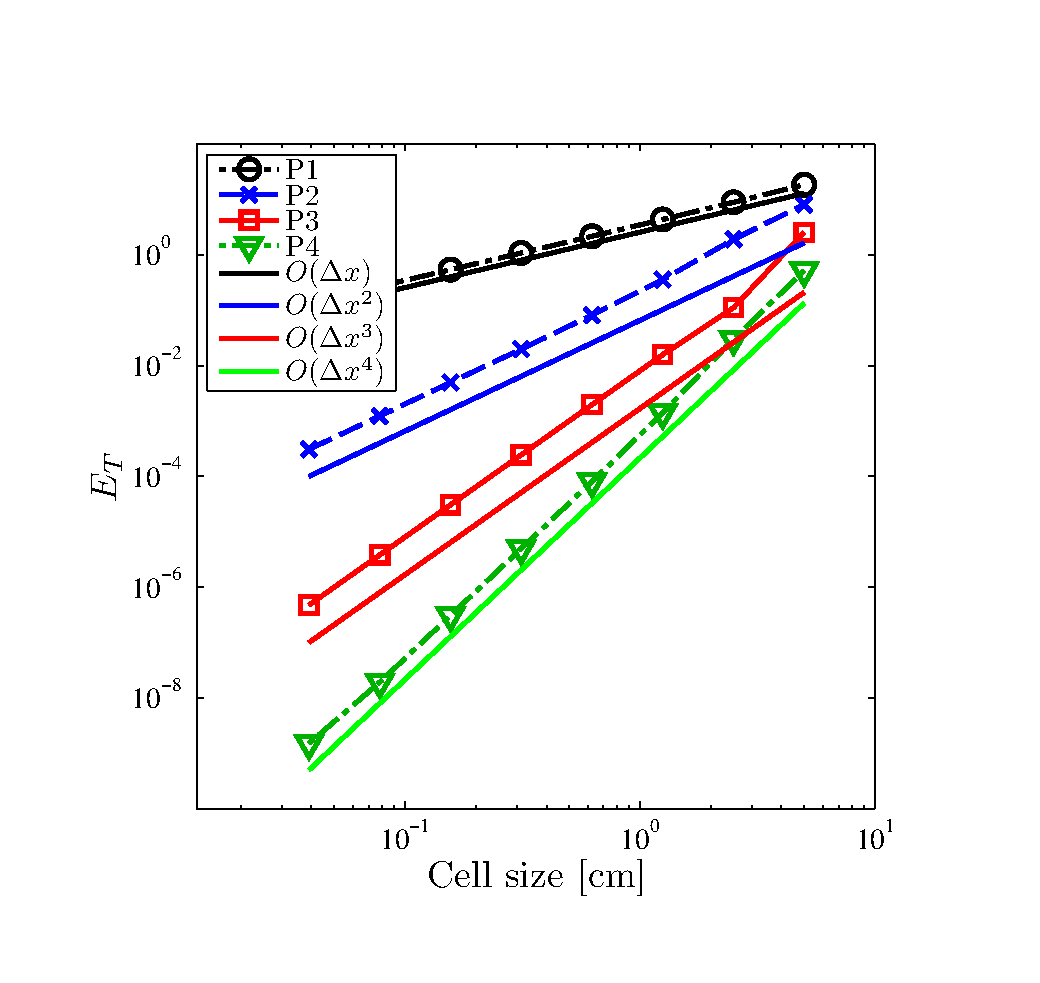
\includegraphics[width=\textwidth,trim=0.25in  0.2in 0.75in 0.5in,clip=true]{../chapter6_grey_radtran/Dissertation_Data/MMS2_SLXS_Lobatto_temp_L2.pdf}
\end{columns}
\end{frame}

\begin{frame}
\frametitle{SL Gauss- MMS1 Results}
SL Gauss picks up an order for $T$?
\begin{columns}[t]
\column{0.5\textwidth}
\centering
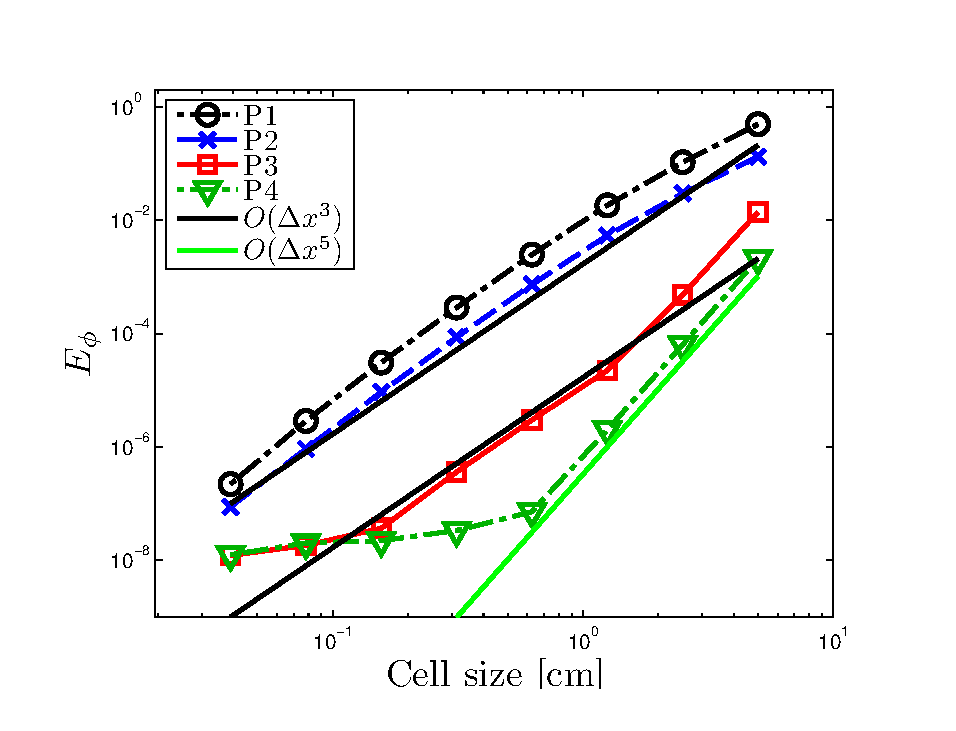
\includegraphics[width=\textwidth,trim=0.25in  0.2in 0.75in 0.5in,clip=true]{../chapter6_grey_radtran/Dissertation_Data/MMS2_SLXS_Gauss_phi_L2.pdf}
\column{0.5\textwidth}
\centering
\includegraphics[width=\textwidth,trim=0.25in  0.2in 0.75in 0.5in,clip=true]{../chapter6_grey_radtran/Dissertation_Data/MMS2_SLXS_Gauss_temp_L2.pdf}
\end{columns}
\end{frame}
\begin{frame}

\frametitle{Steady-state problem}
\bea
M(\mu_d) &=& \frac{1}{4\pi} \\
W_I(x) &=& 19 \cos\left( \frac{\pi x}{2} \right) + 20 \pec \\
W_T(x) &=&  15 \cos\left( \frac{\pi x}{2}  \right) + 20 \pec \\
F(t) &=&  10 \\
C_v &=& 0.1 + 0.2 T^2 \\
\sigma_a &=& \frac{5}{T^2} \\
\sigma_s &=& 0.01 
\eea

\end{frame}

\begin{frame}
\frametitle{SLXS Lobatto $L^2$ Convergence}
\begin{columns}[t]
\column{0.5\textwidth}
\centering
$E_{\phi}$
\includegraphics[width=\textwidth,trim=0.25in  0.2in 0.75in 0.5in,clip=true]{../chapter6_grey_radtran/Dissertation_Data/Constant_Time_SLXS_Lobatto_phi_L2.pdf}
\\
$\propto P+1$
\column{0.5\textwidth}
\centering
$E_{T}$
\includegraphics[width=\textwidth,trim=0.25in  0.2in 0.75in 0.5in,clip=true]{../chapter6_grey_radtran/Dissertation_Data/Constant_Time_SLXS_Lobatto_temp_L2.pdf}
\\
$\propto P$
\end{columns}
\centering
No surprises
\end{frame}

\begin{frame}
\frametitle{SLXS Gauss $L^2$ Convergence}
\begin{columns}[t]
\column{0.5\textwidth}
\centering
$E_{\phi}$
\includegraphics[width=\textwidth,trim=0.25in  0.2in 0.75in 0.5in,clip=true]{../chapter6_grey_radtran/Dissertation_Data/Constant_Time_SLXS_Gauss_phi_L2.pdf}
\\
$\propto P+2$
\column{0.5\textwidth}
\centering
$E_{T}$
\includegraphics[width=\textwidth,trim=0.25in  0.2in 0.75in 0.5in,clip=true]{../chapter6_grey_radtran/Dissertation_Data/Constant_Time_SLXS_Gauss_temp_L2.pdf}
\\
$\propto P+1$
\end{columns}
\centering
\vspace{0.2in}
Where did the extra order in $E_{\phi}$ come from?
\end{frame}

\begin{frame}
\frametitle{$E_{\phi_A}$ Convergence}
\begin{columns}[t]
\column{0.5\textwidth}
\centering
SLXS Lobatto
\includegraphics[width=\textwidth,trim=0.25in  0.2in 0.75in 0.5in,clip=true]{../chapter6_grey_radtran/Dissertation_Data/Constant_Time_SLXS_Lobatto_phi_A.pdf}
\\
TRT $E_{\phi_A}\propto 2P$
\\
Neutronics $E_{\psi_A} \propto 2P$
\column{0.5\textwidth}
\centering
SLXS Gauss
\includegraphics[width=\textwidth,trim=0.25in  0.2in 0.75in 0.5in,clip=true]{../chapter6_grey_radtran/Dissertation_Data/Constant_Time_SLXS_Gauss_phi_A.pdf}
\\ 
TRT $E_{\phi_A} < 2P+2 $
\\
Neutronics $E_{\psi_A} \propto 2P+1$
\end{columns}
\centering
\end{frame}

\begin{frame}
\frametitle{$E_{T_A}$ Convergence}
\begin{columns}[t]
\column{0.5\textwidth}
\centering
SLXS Lobatto
\includegraphics[width=\textwidth,trim=0.25in  0.2in 0.75in 0.5in,clip=true]{../chapter6_grey_radtran/Dissertation_Data/Constant_Time_SLXS_Lobatto_temp_A.pdf}
\\
TRT $E_{T_A}\propto 2P$
\\
Neutronics $E_{\psi_A} \propto 2P$
\column{0.5\textwidth}
\centering
SLXS Gauss
\includegraphics[width=\textwidth,trim=0.25in  0.2in 0.75in 0.5in,clip=true]{../chapter6_grey_radtran/Dissertation_Data/Constant_Time_SLXS_Gauss_temp_A.pdf}
\\
TRT $E_{T_A} \propto 2P+2 $
\\
 Neutronics $E_{\psi_A} \propto 2P+1$
\end{columns}
\centering
\end{frame}

\end{document}
%------------------------------------------------------------------------------